%! TEX option=--shell-escape
\documentclass[12pt,a4paper,openright,twoside]{report}

\usepackage[utf8]{inputenc}
\usepackage[spanish]{babel}
\usepackage{amsmath}
\usepackage{amsfonts}
\usepackage{amssymb}
\usepackage{graphicx}
\usepackage{microtype}
%\usepackage{cite}
\usepackage[numbers]{natbib}

\usepackage{lmodern,textcomp}
%Paquete para ajustar el tamaño de pagina, margenes, etc
\usepackage{geometry}
%geometría definida respecto a las sugerencias
  \geometry{
  	includehead,
  	includefoot,
  	a4paper,
  	left = 20mm,
  	top = 25mm,
  	total ={170mm,257mm},
  }
%El siguiente paquete provee las funciones necesarias para ajustar el encabezado
%y el pie de página
\usepackage{fancyhdr}
  \pagestyle{fancy}
  \fancyhf{} % resetea el encabezado y el pie
  \fancyhead[LE,LO]{\fontsize{9pt}{1pt}\it \leftmark}
  \fancyfoot[LE,RO]{\fontsize{12pt}{1pt}\thepage}


  \fancypagestyle{plain}{
  	\fancyfoot[RE,RO]{\fontsize{12pt}{1pt}\thepage}}

%usado para colocar la fecha en la carátula
\usepackage{datetime}

\setlength{\parskip}{\baselineskip}
%\renewcommand{\topfraction}{.85}
\renewcommand{\bottomfraction}{.7}
%\renewcommand{\textfraction}{.15}
%\renewcommand{\floatpagefraction}{.66}
%\renewcommand{\dbltopfraction}{.66}
%\renewcommand{\dblfloatpagefraction}{.66}

\usepackage{listingsutf8}
%\usepackage{listings}
\lstset{inputencoding=utf8/latin1}
\lstset{tabsize=4}
\usepackage{caption}
\usepackage{subcaption}
\usepackage{enumerate}
\usepackage{lineno}
\usepackage{array}
\usepackage{booktabs}
\usepackage[titletoc]{appendix}
\usepackage[binary-units]{siunitx}
\usepackage{titling}
\usepackage{soul}
\usepackage{adjustbox}

\usepackage{hyperref}
\hypersetup{
	colorlinks=true,
	linkcolor=black,
	filecolor=black,
	urlcolor=black,
	pdftitle={\@title},
	bookmarks=true
}

\usepackage{tikz}
\usetikzlibrary{arrows,backgrounds,decorations.pathreplacing,fit,positioning,petri,babel,shapes,circuits.logic.mux,circuits.logic.US,shapes.gates.logic,trees,patterns}

%\tikzstyle{style} = [definition]
\tikzstyle{interior}=[rectangle,rounded corners,draw=black,minimum size=3em, text width=20,fill=white]
\tikzstyle{exterior} = [rectangle,draw=black,minimum size=40]
\tikzstyle{mode text} = [midway,sloped,text width=200]
\tikzstyle{contenedor} = [rectangle,draw=black]
\tikzstyle{core}=[interior]
\tikzstyle{perif} = [interior,minimum height=20]
\tikzstyle{buf}=[core, text width=53, align=center]
\tikzstyle{obuf} = [buf, node distance=.7]
\tikzstyle{env} = [fill=black!20]
\tikzstyle{simple}=[rectangle, draw=black, minimum height=220, text width=65,align=center]
\tikzstyle{moore} = [rectangle,draw=black, minimum height= 30,text width=80,align=left]
\tikzstyle{mealy} = [rectangle,rounded corners=12, draw=black, text width = 80,align=left,minimum height=40]
\tikzstyle{ask} = [diamond,text width=50,draw=black,align=center,]
\tikzstyle{bloque}=[exterior,align=center,minimum size=60,text width=60]
\tikzstyle{hub}=[draw=black,anchor=west,circle]
\tikzstyle{dev}=[draw=black,anchor=west,rectangle,rounded corners,text width=60,align=center]
\tikzstyle{pid}=[draw=black,align=center,rectangle,rounded corners,minimum width=20,minimum height=120,pattern=north east lines,pattern color=black!35]
\tikzstyle{dir}=[draw,rectangle,rounded corners,minimum width=20,minimum height=120,align=center]
\tikzstyle{data}=[draw=black,align=center,rectangle,rounded corners,minimum width=120,minimum height=120,fill=black!05]
\tikzstyle{crc}=[draw=black,align=center,rectangle,rounded corners,minimum width=20,minimum height=120,pattern=dots,pattern color=black!25]
\tikzstyle{field}=[draw=black,rectangle,rounded corners, minimum height=30,align=center]

\newcommand{\epg}[3]{
	Buffer {#1}\\
	[38.5pt]EP{#2}\\
	[38.5pt]{#3} Bytes}

\newcommand{\ep}[3]{
	Buffer {#1}\\
	[8pt]EP{#2}\\
	[8pt]{#3} Bytes}

\newcounter{wavecount}

\newcommand{\newwave}[1]{
	\path (0,\value{wavecount}) node[text width=70,anchor=east,align=right]{#1} node[coordinate](t_cur){};
	\draw (0,\value{wavecount}+.3) --++(.2,0);
	\draw (0,\value{wavecount}-.3) --++(.2,0);
	\path (t_cur) --++(.3,0)node[coordinate](t_cur){};
	\addtocounter{wavecount}{-1}}

\newcommand*{\bit}[2]{
	\draw (t_cur) -- ++(0.1,.6*#1-.3) -- ++(#2-.2,0) -- ++(+.1,.3-.6*#1)
	node[coordinate] (t_cur) {};}

\newcommand*{\bitvector}[2]{
	\draw[] (t_cur) -- ++( .1, .3) -- ++(#2-.2,0) -- ++(.1, -.3)
	-- ++(-.1,-.3) -- ++(.2-#2,0) -- cycle;
	\path (t_cur) -- node[align=center] {#1} ++(#2,0) node[coordinate] (t_cur) {};}


\DeclareSIUnit[number-unit-product = {}]
\byte{B}

\graphicspath{{./imgs/}}

\renewcommand{\chaptermark}[1]{%
    \markboth{\thechapter.\ #1}{}}

\lstset{literate=
	{á}{{\'a}}1	{é}{{\'e}}1	{í}{{\'i}}1	{ó}{{\'o}}1	{ú}{{\'u}}1	{α}{{$\alpha$}}1	{β}{{$\beta$}}1	{γ}{{$\gamma$}}1	{ñ}{{\~n}}1
}

\renewcommand{\appendixpagename}{Apéndice}
\renewcommand{\labelitemi}{$\bullet$}
\renewcommand{\labelitemii}{$-$}

% Las próximas líneas son archivos que conviene que estén por aquí

	%bridge.c
\newcommand{\bridge}{secciones/cuerpo/capitulo3/bridge.c}
\newcommand{\host}{USB Host}
\newcommand{\device}{Dispositivo USB}
\newcommand{\devices}{Dispositivos}
\newcommand{\ep}{Extremo}
\newcommand{\hub}{Distribuidor USB}
\newcommand{\function}{Función USB}
\newcommand{\functions}{Funciones USB}
\newcommand{\controller}{Controlador USB}


\lstset{literate=
	{á}{{\'a}}1	{é}{{\'e}}1	{í}{{\'i}}1	{ó}{{\'o}}1	{ú}{{\'u}}1	{α}{{$\alpha$}}1	{β}{{$\beta$}}1	{γ}{{$\gamma$}}1	{ñ}{{\~n}}1
}
\title{Comunicación USB 2.0 para sistemas científicos implementados en FPGA}
\author{Edwin Barragán}

\begin{document}
%	\renewcommand{\tablename}{Tabla}
	\begin{titlepage}
  \begin{center}
    \begin{Large}
      \textbf{UNIVERSIDAD NACIONAL DE SAN JUAN\\
      \vspace*{0.05in}
      FACULTAD DE INGENIERIA\\
      \vspace*{0.05in}
      Departamento de Electrónica y Automática\\
      \vspace*{0.2in}
      
\includegraphics[width=.3\textwidth]{logo_unsj.png}\\
      \vspace*{\fill}}
    \end{Large}
    \begin{Large}
      \textbf{Trabajo Final\\\MakeUppercase{\thetitle}} \\
      Informe\\
    \end{Large}
    \vspace*{\fill}
    \begin{large}
      \textbf{\theauthor}\\
      Autor\\
    \end{large}
    \vspace*{0.5in}
    \begin{large}
      \textbf{Ing.~Cristian~Sisterna \hspace*{\fill}
      Mg.~Martín~Pérez \hspace*{\fill} Dr.~Marcelo~Segura \\}
      Asesores\\
    \end{large}
    \vspace{\fill}
    \rule{80mm}{0.1mm}\\
    \vspace{.1in}
    \the\year
  \end{center}

\end{titlepage}

	\null
	\chapter*{Agradecimientos}
  Acá le agradezco a todos los miembros de la prestigiosa y gloriosa Comisión de Trabajo Final por sus incontables aportes a la causa.
  Si pongo punto y meto enter no se vé en el documento.\\
  Si escribo barra barra hago un salto de linea pero no cambio de párrafo.

  Si doy doble enter, coloca sangría, pero no hace el salto de línea para el párrafo.\\

  Este último sí que es un párrafo decente!

	\tableofcontents
	\chapter{Introducción}
	\section{Motivación}
		Un carpintero desea medir la distancia de una barra de madera que luego será, tal vez, la altura de las patas de una futura mesa. Para ello, utiliza una cinta métrica, compuesta de una cinta metálica que posee una escala graduada. Sabe entonces que la barra mide la distancia que coincide con la distancia de la cinta graduada.\\

Un panadero desea medir cuanto pesa la harina que debe para poder amasar. Entonces, la coloca en una balanza y observa cuanto marca su indicador. Así conoce que la masa de la harina es equivalente a la fracción de medida que indica la balanza.\\

Un atleta desea conocer cuanto demora en correr un trayecto que posee \SI{1}{\kilo\metro}. Por esto, registra el valor que indica su reloj al principio del recorrido y cuando alcanza el final observa nuevamente el artefacto. Luego de esto, calcula la diferencia entre el valor final y el inicial, conociendo cuanto tiempo le tomó realizar su travesía.\\

En los tres casos anteriores, tanto el carpintero, como el panadero y el atleta desconocen algo y necesitan cambiar su estado con respecto a esa incertidumbre. Por ello recurren a diferentes objetos, a fin de obtener conocimiento a partir de ellos. Sin embargo, estos objetos, por si mismos, no otorgan información, sino más bien otorgan un dato, que comparado y contrastado con otros datos, se traducen en conocimiento.\\

La información es el resultado de ordenar y procesar un conjunto de datos, de forma tal que permitan cambiar el estado de conocimiento sobre un asunto determinado. En el caso del carpintero, compara el tamaño de las patas de la mesa con una cinta metlálica, que a su vez, posee registrada su distancia en función de algún patrón de metrología, establecido por convención. Esto quiere decir que el dato 1, la longitud del patron, junto al dato 2, escala graduada de la cinta, más el dato 3, la longitud de la cinta métrica, permiten al carpintero cambiar su estado de desconocido a conocido, con respecto a la longitud del trozo de madera, a través de la información proporcionada por el conjunto de datos.\\

Se puede realizar el mismo análisis con respecto a la balanza del panadero, considerando un peso patrón, un desplazamiento y una escala graduada o una señal eléctrica emitida por una celda de carga deformada un porcentaje de su capacidad, registrada previamente por su fabricante conforme a pesos patrones, y un circuito adaptador que transforma esa señal electrica en un valor numérico mostrado en un indicador.\\

El atleta compara las posiciones y los desplazamientos de las agujas de su reloj, previamente calibrado para que dé una vuelta por cada minuto en una aguja, otra aguja que dé una vuelta por hora y la tercera una vez cada 12 horas. Además, es probable que él haya ajustado la hora que indica el reloj para que otorgue un horario idéntico al de referencia, establecido por convención.\\

En todos los casos, se posee una gran cantidad de datos que, ordenados, procesados y comparados otorgan al usuario un valor útil, ya sea una longitud, una masa, un tiempo o cualquiera sea la variable física que se desee conocer.\\

La ciencia es un conjunto de técnicas y procedimientos que, a través del método científico, busca adquirir, descubrir y/o desarrollar nuevo conocimiento. Se desprende entonces, que la ciencia produce, de forma fundamental, información que luego es transformada en conocimiento. Cuando hablamos de ciencia, hablamos de una gran gama de objetos de estudio, sujeto a través del cuál se clasifican, en la mayoría de los casos, las ciencias: las Ciencias Sociales estudian las relaciones humanas, las Ciencias Naturales estudian objetos que se encuentran en la naturaleza, las Ciencias de la Tierra se enfocan en una rama más particular de la naturaleza, como lo son los minerales, la superficie terrestre, etc; y siguiendo así se puede encontrar un sinnuméro se ciencias. Sin embargo, toda ciencia necesita, para su correcta producción científica, adquirir una gran cantidad de datos que luego será nordenados, procesados y transformados en información y conocimiento.\\

La incorporación de una herramienta especialmente diseñada para el procesamiento de datos, como lo es la computadora, permite manejar un numero cada vez creciente de información.
Es por eso que se encuentra en desarrollo un gran número de sensores y dispositivos que permitan obtener cada vez más datos.\\

En este sentido, una de los desarrollo que se encuentran en boga es el sensores que adquieran imágenes. Como ejemplos podemos encontrar, entre muchos otros, el desarrollo de sensores de radiación[1], ultrasonografía[2], telescopía de objetos cercanos[3], imagenes de distancia[4].





[1][https://ieeexplore.ieee.org/abstract/document/8214376]
[2][http://www.idr.iitkgp.ac.in/jspui/bitstream/123456789/9068/1/NB15975_Abstract.pdf]
[3][https://ieeexplore.ieee.org/abstract/document/8396725]
[4][https://www.sciencedirect.com/science/article/pii/S0030402617316029]




El mundo actual, en el que vivimos inmersos, demanda y consume volumenes cada vez más grandes de información. Con solo hacer una rapida miradad en diarios, incluso no especilizados, se observa la importancia que poseen las ciencias y disciplinas que manejas la informacion, aquellas areas agrupadas dentro del conjunto Técnico de la Información y la Comunicación, o más ocnocido por sus siglas, TIC's.

Internet de las cosas , Big Data, Inteligencia Artificial, Redes Neuronales, Robótica, Domótica, entre otras, son areas en las que los datos y la información es abultada y su correcto manejo es sumamente complejo e importante. Además, ninguna de las actividades científicas, puede escapar de esta gran demanda mundial de información.

La información es un conjunto de datos ordenados y procesados de forma tal que permita al que lo lea que eleve su nivel de conocimiento sobre un determinado tema. Es decir que, para que exista información, en primer lugar tenemos que tener datos, de forma tal que podamos luego procesarlos y obtener realmente información de llos.

Como ejemplo de esto, podemos citar simplemente el acto de medir la presión dentro de un tubo de gas. Sería normal pensar en que, teniendo este objetivo en mente, simplemente coloquemos un manómetro en la salida del tubo. El manómetro es un artefacto que posee una varilla 





El mundo, durante la era de la información, nos exige producir y consumir cada vez más y más información. En cada aspecto social dela vida de la persona se pueden encontrar ejemplos claros de esto.\\

Bajo un punto de vista social nos vemos bombardeados por información. Los 'influencers' que se mueven a traves de Facebook, Twiter, Instagram, Snapchat, Linkedin, Youtube, etc, necesitan para estar a la moda, producir constantemente material y que ese material sea consumido por alguien que este demandando esa información.

En el area de econimía y finanzas existen cada vez más robots que extraen información de las diferentes bolsas, periodicos, bancos, industrias y donde se ocurra que pueda haber información útil, para tomar mejores decisiones que, por supuesto, también ejecutan los robots.

En el comercio, desde las tiendas de supermercado hasta las tiendas digitales que trabajan solo a través de internet están constantemente recabando datos y procesandolos a din de diseñar estrategias que permitan ofrecer productos que se adapten mejor a lo que busca el cliente y de esa forma lograr vender mayores volumenes.

La industria cuenta cada vez más con multiplicidad de posibilidades basadas en sensores que adquieren grandes cantidades de datos que son almacenadas y procesadas, muchas vecen 'en línea' o 'al instante', de forma tal de encontrar mejores procesos o ejecutar nuevas tareas, como por ejemplo la industria automotriz, enfocada cada vez más en autos que puedan manipular todo el entorno y ser totalmente autónomos de un conductor.
La industria espacial y satelital dotan a sus equipos de mayores sensores y mayores flujos de datos. La industria médica brinda cada vez más posibilidades de diagnóstico a traves de nuevas técnicas y formas de adquisición de imágenes.

A todo esto, la ciencia y el desarrollo de nuevas aplicaciones y equipos, no son indiferente. Cada vez se encuentran más innovaciones y desarrollos de nuevos sensores que adquieren flujos de información crecientes. La toma de imagenes se ha vuelto una herramienta clave para la investigación en diversas areas, tales como la biología, la ciencia de materiales, las ciencias nucleares, las ciencias de la tierra, etc.

Las redes sociales son un ejemplo de esto, pero esto se observa en la industria, la economía, las finanzas e incluso hasta en la casa.



[1] file:///home/lechuzin/Facultad/Trabajo%20Final/lechuzing/docs/bibliografia/The-Rise-of-the-Network-Society-With-a-New-Preface-Volume-I-The-Information-Age-Economy-Society-and-Culture-Information-Age-Series-.pdf
 
	\chapter{Bus Serial Universal 2.0}
	\label{cap:usb}
	El Bus Serial Universal, o USB por sus siglas en inglés, es un sistema de comunicación diseñado durante los años 90 por seis fabricantes vinculados a la industria informáticas, Compaq, Intel, Microsoft, Hewlett-Packard, Lucent, NEC y Philips, con la idea de proveer a su negocio de un sistema que permita la conexión de PCs con teléfonos y periféricos con un formato estándar, fácil de usar y que permita la compatibilidad entre los distintos fabricantes.\\

Hasta ese momento, el gran ecosistema de periféricos, sumado a los nuevos avances y desarrollos, hacia muy compleja la interoperatividad de todos ellos. Cada uno de los fabricantes desarrollaba componentes con características, tales como fichas, niveles de tensión, velocidades, drivers, lo cuál dificultaba al usuario estar al día y poder utilizar cada componente que compraba. Esto también complicaba a las mismas empresas productoras, por que la introducción de un nuevo sistema requería de mucho soporte extra para poder conectar todo lo ya existente.\\

Todo esto, quedó saldado con el aparición de la norma USB que, gracias a la gran cuota de mercado de sus desarrolladores, fue adoptado en forma rápida y se transformó en la especificación por defecto a la hora de seleccionar un protocolo. Al punto tal esto se cumplió que hoy, más de 20 años después, es muy difícil encontrar PC's con otro tipo de puertos, salvo que, en el momento de su compra, se solicite especialmente un puerto determinado. Así, cualquier PC nueva disponible en el mercado debe poseer puertos USB para la conexión de los periféricos.\\

El diseño de la norma USB busca resolver tres problemáticas interreacionadas, que son: La conexión de teléfonos con las PC, la facilidad de uso, es decir, que el usuario solo conecte su dispositvo y pueda utilizarlo, y la expansión en la cantidad de puertos disponibles para conectar periféricos\cite{USBspec}. Para satisfacer estas tres demandas, la norma USB 2.0 busca alcanzar un conjunto de metas que apuntan a la facilidad del uso, la compatibilidad entre versiones diferentes de la misma tecnología, la robustez en el flujo de datos, y la convivencia de diferentes configuraciones temporales en único bus, provistos de una interfaz estándar, ancho de banda que soporte comunicaciones audiovisuales de calidad aceptable y un bajo coste.\\

El presente capitulo intenta ser un breve resumen con los aspectos más relevantes de la norma en cuanto a su composición física, su topología, los dispositivos que intervienen, la importancia de los mismos y como los datos son transmitidos desde y hacia una PC.\\

%	Desde el punto de vista técnico, el protocolo USB es un sistema del tipo maestro-esclavo, donde el maestro, denominado {\it HOST}, debe ser necesariamente una PC (o un dispositivo con software y hardware capaces de incorporar los drivers necesarios) y cualquier periférico a ella acoplada será un esclavo\cite{USBspec}.\\
%	
%	Para describirlo es conveniente diferenciar tres partes. Una capa física, en donde se definen los componentes que intervienen, una capa de protocolo, en donde se define el formato, el marco en el que son enviados los paquetes, como se direccionan y como se comunican entre sí, y una parte lógica, en donde cada componente es visto solamente como un extremo y define como fluyen los datos desde un extremo hacia la PC y viceversa.\\
%	
%	\subsection{Capa física}
%		
%	\begin{figure}[!ht]
%		\centering
%		\begin{tikzpicture}[scale=1.2\textwidth/\paperwidth,>=latex]
%			\begin{scope}
%				\begin{scope}[transform shape,node distance=2,grow=right,sibling distance=80, level distance=30]
%					\node[draw=black] (host) {\it HOST}
%						child {node[hub] (root) {Raiz} edge from parent[level distance=70,<->]
%							child{node[hub](hub){HUB} edge from parent [<->,sibling distance=35,level distance=50]
%								child {node	[dev]	(out){Función} edge from parent [<-]}
%								child {node	[dev]	(in){Función} edge from parent [->]}
%								child {node (text) {Dispositivo compuesto} edge from parent [draw=black!0]}
%							}
%							child{node[dev]{Función} edge from parent [->]}
%							child{node[dev]{Función} edge from parent [<-]}
%						};
%				\end{scope}
%				\begin{scope}
%					\node[draw=black,rounded corners, dashed, fit=(hub)(out)(in)(text)]	(comp)	{};
%				\end{scope}
%			\end{scope}
%		\end{tikzpicture}
%		\caption{Topología de un sistema USB}
%		\label{fig:arqusb}
%	\end{figure}
%		
%	En esta sección no se describirán los detalles de las conexiones eléctricas ni mecánicas a las que se refieren las especificaciones de la norma USB debido a dos cuestiones fundamentales. Una de ellas es que toda esta sección de la norma está resuelta ya por los fabricantes de la interfaz que se utiliza en este trabajo. A su vez, maneja todas las señales, arma y desarma los paquetes que salen hacia la PC y que llegan de ella respectivamente. Por otro lado, no es el objetivo de este trabajo adentrarse en esos detalles. Gracias a la extensión de este tipo de comunicación existen una gran cantidad de fabricantes en el mercado que fabrican cada uno de los componentes, ya sean, cables, conectores en todas sus versiones, adaptadores de un tipo de estos, su costo es despreciable con respecto a cualquier tipo de desarrollo en ese sentido y son de una muy buena calidad, es decir que todos cumplen con lo que la norma establece. Sí, se describen los dispositivos físicos y su categoría, según la norma, en función del rol que cumplen.\\
%	
%	La comunicación USB posee una topología maestro-esclavo. Es decir, existe un dispositivo que dirige todas las transferencias de datos y otros que responden a sus directivas. Por esto, el elemento central de cualquier comunicación USB es el {\it HOST} (director o anfitrión, por su traducción de la voz inglesa). Él es el que posee el {\it Host USB Controller}\cite{USBspec}. Esto quiere decir que tiene la capacidad de registrar los dispositivos acoplados, asignarles dirección, colocar los paquetes de salida y/o llegada en sus respectivas listas y servilos a los procesos que utilizan esta comunicación. Además, el {\it HOST} se encarga de enviar los tokens a todos los periféricos, con la dirección del dispositivo, el sentido de la comunicación, el tipo de transferencia que se espera y todas las acciones de control que el sistema requiera. En la mayoría de los casos, el {\it HOST} es una PC, auqnue también puede ser cualquier dispositivos  ``inteligente'' como un smartphone.\\
%	
%	En el otro extremo de la comunicación, se encuentran lo que la norma denomina {\it funciones}\cite{USBspec}. Las {\it funciones} son todos los periféricos que actúan como fuente o sumidero de información. Es decir, en caso de periféricos de entrada, serán una fuente de datos hacia el {\it HOST}. Si los periféricos son de salida, serán un sumidero de la información que proporciona la PC. Los casos de periféricos de entrada/salida, se denominan {\it dispositivos compuestos}.\\
%		
%	Existe también, a los fines de la norma,un elemento intermedio, denominado {\it HUB} (concentrador o distribuidor, según la traducción del inglés). Este dispositivo se encarga de conectar dos o más {\it funciones}, ya sea de entrada o salida, de recibir y enviar las direcciones y de regenerar las señales que el {\it HOST} envía y deben ser recibidas por las {\it funciones}.\\
%	
%	La Figura \ref{fig:arqusb} muestra la topología típica de un sistema USB. En ella, se observa el {\it HOST} como un rectángulo, las {\it funciones} como rectángulos con los bordes redondeados y los distribuidores como círculos. Se puede notar que el {\it HOST} posee un distribuidor propio llamado {\it Raiz} en el cual se conectan todos las {\it funciones} y distribuidores. Cada {\it Función}posee una única dirección. Pueden existir dispositivos que posean funciones diversas con un mismo encapsulado, como por ejemplo un auricular que tenga micrófono incorporado. Este dispositivo, tendrá un {\it HUB} que concatena dos {\it funiones} diferentes.\\
%	
%	\subsection{Capa lógica}
%	Desde el punto de vista lógico, cada dispositivo es visto por el {\it HOST} como un extremo (EP, del inglés, {\it endpoint}) independiente, que posee solo un modo de comunicación, es decir, el protocolo se comunicara solo por un tipo de transferencia y en un único sentido con cada {\it EP}. En otras palabras, USB registra un periférico de entrada/salida como un {\it EP} de entrada y otro de salida en forma independiente.\\
%	
%	Esta independencia brinda la posibilidad de configurar cada extremo de forma diferente y obtener el ancho de banda necesario para la subida y bajada de datos, los tiempos de acceso al bus, la dirección y todo lo relacionado a los modos de comunicación conforme a los requerimientos.\\
%	
%	El protocolo entiende que entre le {\it HOST} y cada uno de los extremos existe un tubo (la norma en ingles habla de {\it pipes}) en donde la información es colocada y transferida. Luego, cada tubo posee la configuración establecida por el controlador del {\it HOST} y se comunica con cada {\it EP} por medio de estos tubos. A los fines del usuario, esto es lo importante, por cuanto se solicita acceso al bus y define en que buffer va a contener los datos a enviar o transmitir y el protocolo se encarga de el empaquetado, el armado de los cuadros, el acceso el bus y el posterior envío de datos.\\
%	
%	\subsection{Capa de protocolo}
%	En la capa de protocolo, la especificación de la norma detalla cómo se compone un cuadro y cómo deben ser estructurados los paquetes para que sean efectivamente enviados a través del sistema. Cada mensaje que se intercambia por el bus se denomina paquete. Cada paquete puede poseer hasta cinco campos, dependiendo del tipo de paquete que sea enviado a través del sistema y de quien sea el remitente. A su vez, cada paquete comienza con una señal de sincronismo ({\it SYNC}) y un Comienzo de Paquete (SOP de {\it Start-of-Packet}), y terminan con una señal de Fin de Paquete (EOP por {\it End-of-Packet}).\\
%	
%	Por otra parte, los paquetes está temporalmente encapsulados en cuadros. Cada cuadro posee un Comienzo de Cuadro (SOF, {\it Start-of-Frame}) y posee una duración de \SI{1}{\milli\second}, hasta el próximo SOF. En las comunicaciones de alta velocidad, es decir, aquellas que poseen una tasa de bit de \SI{480}{\mega\bit\per\second}. Se subdivide un cuadro en 8 micro-cuadros de \SI{125}{\micro\second} cada uno.\\
%	
%	\subsubsection*{Campos de Paquetes}
%	Cada paquete contiene un campo denominado identificador de paquete (PID del inglés {\it Packet Identifier}). El PID indica el tipo de paquete que se está enviando y, como consecuencia, el formato de cada uno, es decir, que campos acarrea y que control de datos utiliza.
%	
%	A su vez, cuando el host solicita algo al sistema, lo realiza a través del denominado campo de dirección. Este campo, se compone de dos partes, la primera es el campo de dirección de la función y el segundo es la dirección de extremo.\\
%	
%	Los mensajes de datos, poseen un campo dedicado de forma específica a los datos. Puede poseer un numero entero de bytes, desde \SI{0}{} a \SI{1024}{}.\\
%	
%	Para corroborar el envío de datos, USB utiliza verificación de redundancia cíclica (CRC o {\it Cyclic Redundancy Checks}). Los paquetes especiales y los de token poseen un verificador  CRC5, es decir, de 5 bits, cuyo polinomio generador es:
%	
%	\begin{center}
%		\begin{math}
%			G(X) = X^5 + X^2 + 1
%		\end{math}
%	\end{center}	
%	
%	Por su parte, los paquetes de datos, poseen CRC16, ya que pueden llegar a ser bastante extensos. En su caso, el polinomio generador está dado por:
%	
%	\begin{center}
%		\begin{math}
%			G(X) = X^{16} + X^{15} + X^2 + 1
%		\end{math}
%	\end{center}
%	
%	Existe un campo relativo a los cuadros temporales, que se denomina campo de número de cuadro. Este es enviado por el {\it HOST} en cada SOF y es incrementado a cada cuadro. Los micro-cuadros también poseen un número de cuadro, sin embargo, este es aumentado solamente cada 8 micro-cuadros, es decir, el número se incrementa cada \SI{1}{\milli\second} y se repite durante los 7 micro-cuadros de \SI{125}{\micro\second}, en comunicaciones de alta velocidad.\\
%	
%	\subsubsection*{Formato de paquetes}
%	
%	%TODO quedé por acá..
%	\begin{figure}[t]
%		\centering
%		\begin{tikzpicture}[scale=\textwidth/\paperwidth,>=latex]
%			\begin{scope}
%				\begin{scope}[transform shape,node distance=.15]
%					\node[pid]	(pidtok)	{P\\I\\D\\\ \\T\\o\\k.};
%					\node[dir]	(adtok)	[right=of pidtok]	{D\\i\\r.};
%					\node[dir]	(eptok)	[right=of adtok]	{E\\x\\t\\r.};
%					\node[crc]	(crc5)	[right=of eptok]	{C\\R\\C\\5};
%				\end{scope}
%				\begin{scope}
%					\node[exterior,minimum size=0,inner sep=1,fit=(adtok)(eptok)](tokad){};
%					\node[below=.01 of tokad.south,align=center,transform shape] (texttok){Paquete\\Token};
%					\node[exterior,inner sep=1,fit=(pidtok)(tokad)(crc5)(texttok)](pkttok){};
%				\end{scope}
%				\begin{scope}[transform shape,node distance=.15]
%					\node[pid,node distance=.4]	(piddat)	[right=of crc5]{D\\a\\t\\a\\\ \\P\\I\\D};
%					\node[data]	(data)	[right=of piddat]	{Datos\\útiles};
%					\node[crc]	(crc16)	[right=of data]	{C\\R\\C\\1\\6};
%				\end{scope}
%				\begin{scope}
%					\node[below=.01 of data.south,align=center,transform shape] (textdat){Paquete\\de Datos};
%					\node[exterior,inner sep=2,fit=(piddat)(data)(crc16)(textdat)]{};
%				\end{scope}
%				\begin{scope}[transform shape,node distance=.15]
%					\node[pid,node distance=1.5]	(hspid)	[right=of crc16]{H\\S\\\ \\P\\I\\D};
%				\end{scope}
%				\begin{scope}
%					\node[below=.01 of hspid.south,align=center,transform shape] (texths){Paquete\\de Handshake};
%					\node[exterior,inner sep=2,fit=(hspid)(texths)]{};
%				\end{scope}
%			\end{scope}
%		\end{tikzpicture}
%		\caption{Distintos tipos de paquetes USB}
%		\label{fig:usbpkts}
%	\end{figure}
%	
%	\begin{itemize}
%		\item {\bf Paquetes Token:} A través de este tipo de paquetes el host envía las directivas a los distintos periféricos. Estas directivas pueden ser IN, cuando solicita datos de un periférico; OUT, cuando se dispone a enviar datos hacia una {\it función}; SOF, que indica el inicio de cada cuadro, para que cada función se sincronice y SETUP, cuando va a enviar un paquete de configuración a algún extremo.
%		\item {\bf Paquete de Datos:} Este tipo de PID puede ser emitido por un dispositivo, si es que envía datos al host o bien por el mismo host cuando el flujo de datos es a la inversa.
%		\item {\bf Paquete de {\it Handshake}:} Es enviado por el receptor del mensaje y le informa al emisor el estado de la transferencia. ACK significa que el paquete fue recibido sin errores; NAK, los datos poseen error o el emisor no puede enviar; la señal STALL quiere decir que la solicitud no es soportada o que el extremo está detenido; NYET implica que no hay respuesta aún por parte del receptor.
%		\item {\bf Paquetes Especiales:} Son paquetes con propositos específicos. Con ellos se señalan preambulos emitidos por el {\it HOST}, se informan errores, se solicitan mensajes divididos en diferentes paquetes y se intercambia señales de ping para conocer el estado de los componentes del sistema.
%	\end{itemize}
%	
%	Cada uno de los tipos de paquetes posee un formato específico, tales como se muestran en la Figura \ref{fig:usbpkts}. En ella se observa que los paquetes de token envían un PID, una dirección y un CRC5; los paquetes de datos, se componen de un PID, los datos transmitidos y un CRC16; en el caso de los paquetes de Hanshake, solo el PID indica que tipo de mensaje se envía. Los paquetes especiales no se detallan ya que el formato es muy variable, en función del paquete.\\
%	
%	\subsection{Flujo de datos}
%	Como se menciono anteriormente, el host envía un toquen SOF que sirve para sincronizar los dispositivos al bus. En un sistema USB, el host provee la base de tiempo y envía cada \SI{1}{\milli\second} un SOF (Start of frame, o su traducción, inicio de cuadro) seguido de un numero de 11 bits que sirve para contar cada uno de los marcos. Además, en sistemas de alta velocidad, cada cuadro se divide en ocho microcuadros de \SI{125}{\micro\second}, que también son marcados por un SOF, sin embargo, el contador no se actualiza por cada microcuadro.\\
%	
%	Luego de esto, el sistema puede comenzar con la transferencia de datos. USB dispone 4 tipos de posibles transferencias, que se detallan un poco más adelante, y que pueden ser usadas conforme a los diferentes requerimientos del sistema.\\
%	
%	Cada transferencia de datos está compuesta por un primer paquete de token, emitido por el host, que posee el tipo de transferencia que se espera, sea de entrada, de salida, de control o especial; la dirección de la función que debe responder o recibir el mensaje enviado por el bus y los verificadores CRC5.\\
%	
%	Luego, el siguiente paquete posee los datos que se transfieren, precedido por un PID de datos, y verificadores CRC16. Este paquete es transmitido por el emisor de los datos. Finalmente, el receptor devuelve un paquete de {\it handshake}, indicandole al emisor si el transferencia fue efectiva o no.\\
%	
%	\subsubsection*{Transferencias por paquetes (Bulk transfers)}
%		Este tipo de transferencias puede ser dispuesta para trasmitir un gran flujo de datos. No posee perdida de datos gracias a un sistema de chequeo y retransmisión de datos. El inconveniente que presenta este tipo de transferencias es que en un nivel de prioridades se presenta en el final del sistema. Es decir, el bus solo va a ser usado para transferir este tipo de datos siempre que se encuentre desocupado, o bien, se le asignará una proporción ínfima de ancho de banda para poder trasnmitir con este modo. Es comunmente usado para trasmitir datos que no son críticos en tiempo, por ejemplo para scanners e impresoras.\\
%	
%	\subsubsection*{Transferencias de interrupción}
%		Este tipo de transferencias sirve para enviar y recibir paquetes de datos que requieren un buen sistema de control de errores, pero que, son más restrictivos en tiempos. El sistema siempre destinará un intervalo fijo de tiempo para transmitir los datos que estén pendientes para trasnferencias de interrupción.\\
%	
%	\subsubsection*{Transferencias Isocrónicas}
%		Este tipo de transferencias está destinado a datos que son críticos en tiempo. Es usado, principalmente para enviar datos ``a chorro'', como ser el caso de {\it streaming} de audio o video, en donde los datos producidos deben ser rápidamente llevados al usuario.\\
%	
%		No posee un control de errores muy sofisticado, más que un simple código CRC, pero no existe mecanismo de retransmisión de datos ni handshake entre los {\it EP} y el {\it HOST}.\\
%	
%		Como el tiempo es el requerimiento crítico en este tipo de datos, el controlador le asigna una determinada cantidad de tiempo de bus, o en otras palabras, una determinada cuota de ancho de banda.\\
%	
%	\subsubsection*{Transferencias de control}
%		Este tipo de transferencias solo las emite el host y el sistema las utiliza para configurar cada dispositivo. Debido a su criticidad, el controlador dispondra encada cuadro de una fracción de ancho de banda para las trasnmisiones de control. Es el tipo de transferencias que posee el sistema de detección de errores más sofisticado, de forma tal de asegurar la integridad de los datos de control.\\
%	
%		A cambio de esto, solo muy poca información puede ser trasmitida por cada cuadro, de hasta 64 bytes en sistemas de alta velocidad.\\


%		\section{Objetivos y metas de la norma USB 2.0}
%			\label{usb:obj}
%			\subsection{Objetivo Principal}
	El objetivo del presente trabajo es obtener una comunicación USB 2.0 de alta velocidad entre una PC y un FPGA.%\\
	
	Esta comunicación debe realizarse y documentarse de forma tal que pueda ser usado posteriormente en aplicaciones científicas desarrolladas con FPGA's.
	
\subsection{Objetivos Particulares}
	Para la consecución del objetivo general, se deben cumplir los siguientes objetivos particulares:
	
	\begin{itemize}
		\item Comprender el funcionamiento del protocolo USB.
		\item Seleccionar los componentes a utilizar.
		\item Configurar los componentes seleccionados.
		\item Desarrollar un núcleo en VHDL que sirva de interfaz.
		\item Diseñar e implementar la interconexión de los componentes seleccionados.
		\item Verificar el sistema desarrollado.
		\item Desarrollar un documento que explique el modo de uso del código VHDL utilizado.
	\end{itemize}
%		\section{Objetivos de la norma USB}
		\section{Descripción general de un sistema USB}
			\label{usb:desc}
			USB posee un esquema de bus maestro-esclavo, en forma de árbol cuyo nodo principal es el host. Es decir, la comunicación se realiza siempre a través de una sola línea de comunicación a la que se conectan todos los dispositivos que se necesite (dada el campo de direcciones provisto por la norma, 128 dispositivos como máximo). De esta manera, solo puede transmitir un dispositivo a la vez.\\

El acceso al bus, es decir, el acceso a la línea única compartida de comunicación, es administrado por un maestro. El maestro se encarga de solicitar a cada uno de los dispositivos su intervención. Posteriormente, el dispositivo debe responder al pedido del maestro. Este esquema es lo que se conoce como maestro-esclavo.\\

En un sistema USB no cualquier dispositivo puede ser maestro. Este rol lo cumple solo uno: una PC, o cualquier dispositivo con capacidad de llevar a cabo las tareas asignadas (que se detallan más adelante); denominado Host por la norma. La palabra {\it HOST} proviene del habla inglesa y se traduce como anfitrión, aunque en la jerga se conoce comunmente por su nombre en inglés.\\

\begin{figure}[]
	\centering
	\begin{tikzpicture}[scale=.87,>=latex,level 1/.append style={level distance = 2ex},level 2/.append style={level distance = 40}]
		\begin{scope}
			\begin{scope}[transform shape,grow = down]
				\node[] (host) {\it HOST} [
				sibling distance=60,
%				growth parent anchor=south, 
%				edge from parent fork down,
				]
				child{node[](l1r){Raíz}edge from parent[draw=none]
					child{node[](l2h1){Hub}
						child{node[](l3f1){Función}
						}
						child{node[](l3h1){Hub}
							child{node[](l4h1){Hub}
								child{node[](l5h1){Hub}
									child{node[](l6f1){Función}
									}
									child{node[](l6h1){Hub}
										child{node[](l7f1){Función}
										}
									}
								}
								child{node[](l5f1){Función}
								}
							}
						}
						child{node[] (l3f2) {Función}}
					}
					child{node[](l2f1){Función}}
					child{node[](l2h2){Hub}
						child{node[](l3h2){Hub}
							child{node[](l4f1){Función}
							}
							child{node[](l4f2){Función}
							}
						}
					}
				};
				\node[](l6)[left=of l6f1]{Grada 6};
				\node[](l7)at(l6|-l7f1){Grada 7};
				\node[](l5)at(l6|-l5h1){Grada 5};
				\node[](l4)at(l5|-l4h1){Grada 4};
				\node[](l3)at(l4|-l3f1){Grada 3};
				\node[](l2)at(l3|-l2h1){Grada 2};
				\node[](l1)at(l2|-l1r){Grada 1};
			\end{scope}
			\begin{scope}[dashed]
				\draw (l7) -| (l7f1.west);
				\draw (l6) -| (l6f1.west);
%					\draw(l6f1)--(l6h1);
				\draw (l5) -| (l5h1.west);
%					\draw(l5h1)--(l5h1);
				\draw (l4) -| (l4h1.west);
%					\draw(l4h1)--(l4f1);
%					\draw(l4f1)--(l4f2);
				\draw (l3) -| (l3f1.west);
%					\draw(l3f1)--(l3h1);
%					\draw(l3h1)--(l3f2);
%					\draw(l3f2)--(l3h2);
				\draw (l2) -| (l2h1.west);
%					\draw(l2h1)--(l2f1);
%					\draw(l2f1)--(l2h2);
				\draw (l1) -| (l1r.west);
			\end{scope}
		\end{scope}
	\end{tikzpicture}	
	\caption{Topología de un sistema USB}
	\label{fig:top}
\end{figure}

La topología del bus, cómo se observa en la Figura \ref{fig:top}, posee forma de árbol, es decir, puede ser pensada como una comunicación vertical, donde en el punto más alto se encuentra el Host. Siguiendo hacia abajo, el bus puede encontrar dos tipos diferentes de dispositivos: Funciones, cuyo rol es el de proveer una utilidad al sistema, como ser la de captura de imagen, reproducción de audio o el ingreso de comandos; y Hubs (concentradores o distribuidores), que se encargan de conectar una o más funciones al sistema. La norma USB establece gradas, en donde cada Hub introduce una nueva grada que contiene a las Funciones conectadas. Por cuestiones de restricciones temporales y tiempos de propagación en los cables, no se permiten más de 7 gradas, incluyendo al Host en la primera. Es decir, no se puede conectar más de 5 Hubs en cascada. La grada 7 sólo puede contener Funciones\cite{USBspec}.\\

\begin{figure}[b]
	\centering
	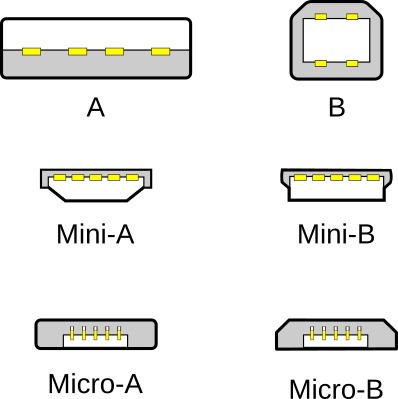
\includegraphics[width=0.28\textwidth]{usbconector}
	\caption{Tipos de conectores USB. Los tipo A deben ser usados en el extremo del Host y los tipo B hacia los periféricos\cite{USBHardwareWiki}}
	\label{fig:con}
\end{figure}

Cada uno de estos dispositivos diferentes, se inteconectan entre sí a través de cables y conductores específicos, diseñados en forma tal que no sea posible conectarlos en forma equivocada. Para cumplir con la norma, el Host debe tener siempre un zócalo compatible con conectores tipo A y los periféricos para enchufes de tipo B. Se observan las diferencias entre uno y otro en la Figura \ref{fig:con}
%		\section{Dispositivos USB}
%			\label{usb:dispo}
		\section{Dispositivos que componen un sistema USB}
			\label{usb:disp}
			Dentro de un sistema USB existen tres tipos diferentes de dispositivos: Host, Hubs y Funciones. Cada uno de ellos tiene asignado un rol específico dentro de la comunicación. Se detallan a continuación las tareas pertinentes a cada uno de ellos.\\

\subsection{Host USB}
	El Host es quien comanda las comunicaciones. Este dispositivo debe tener capacidades de memoria y procesamiento necesarias para almacenar y ejecutar el software de control. A su vez, necesita de hardware que le permita llevar un monitoreo y control de los eventos que suceden en el bus. Entre las tareas que debe llevar a cabo, se encuentran:
	
	\begin{itemize}
		\item Detectar la conexión y desconexión de dispositivos.
		\item Administrar el flujo de los comandos de control con los diferentes dispositivos.
		\item Administrar el flujo de la información entre él (Host) y los diferentes dispositivos.
		\item Llevar estadísticas de actividad y estado del bus.
		\item Proveer potencia a los dispositivos conectados, cuando estos así lo requieran.
	\end{itemize}
	
	Debido a que las tareas que ejecuta el Host requiere una cantidad de recursos de almacenamiento y procesamiento, es usual que el sea una PC la que lleve el rol. El Host es quien inicia la comunicación con las Funciones. Las Funciones, a su vez, responden a lo que fue solicitado por el Host, cuando él lo indique.\\
	
\subsection{Hubs USB}
	Un Hub USB tiene la función de proveer puertos al bus. El primer Hub esta incorporado en el Host y cada vez que se requiere más puertos a los cuales incorporar periféricos, se puede ir agregando a través de Hubs. Otra función importante es la de servir como interfaz entre dispositivos con diferentes velocidades, optimizando así el ancho de banda disponible para la comunicación.\\
	
\subsection{Funciones USB}
	La norma define como Función a todo aquel dispositivo que se conecta al bus y brinda al Host la capacidad de realizar una nueva tarea. Por ejemplo, un teclado otorga un método de entrada adicional, un mouse permite manejar un puntero de la interfaz gráfica, un parlante y un micrófono posibilitan la emisión y recepción de sonidos, respectivamente. Cada una de estas utilidades, compone una Función USB. A su vez, un dispositivo que brinda más de una capacidad es visto por el Host como Funciones separadas conectadas a través de un Hub. Por ejemplo, si se piensa en unos auriculares con micrófono, como los usados por una operadora en un centro de llamados, aunque se presenten integrados en un mismo producto y tengan un único puerto de conexión al bus, el Host los considera como dos Funciones separadas. Las Funciones, desde un punto de vista de software, son independientes unas de otras, por lo que cuando un programa, llamado cliente, necesita utilizar una de ellas, puede acceder a ésta directamente sin conocer cuantas y cuales funciones diferentes existen en el bus.\\
	
	Cada Función se compone de un conjunto de extremos. Un extremo es una porción de dispositivo identificable en forma unívoca\cite{USBspec}. Cada extremo tiene características definidas por el diseñador del sistema que deben estar adecuadas a los requerimientos de cada dispositivo. Los extremos tienen un solo sentido de comunicación y un tamaño máximo de mensaje a transmitir o recibir. Cuando se conecta al bus, un dispositivo debe enviar una descripción en donde consten sus extremos y las diferentes formas de configuración de cada uno, con el tipo de mensajes que soporta, el sentido de la comunicación, el tamaño, entre otros parámetros. Esta descripción se lleva a cabo través de lo que la norma llama descriptores.\\
	
	Todo dispositivo debe contener un extremo con dirección cero dedicado exclusivamente al control de la Función por parte del Host. Debe, como mínimo, poder comunicarse a velocidad completa, es decir, con una señal de \SI{12}{\mega\bit\per\second} y, a su vez, responder a los comandos de control básicos cómo adquirir la dirección, recibir la configuración y enviar los descriptores del dispositivo y sus diferentes configuraciones. Dependiendo de las diferentes requerimientos, el dispositivo puede incorporar otros extremos (15 de entrada y 15 de salida como máximo). Cada extremo no-cero tiene diferente latencia, acceso al bus, ancho de banda, manejo de errores, tamaño máximo de paquete soportado y dirección.\\
	
	
%	punto de vista lógico, cada periférico posee canales únicos de comunicación con el host, llamados tuberías ({\it pipes} en el idioma inglés de la norma). Existen dos tipos de tuberías, las de control, por donde circulan mensajes propios del protocolo y sirven para la administración, configuración y gestión de las comunicaciones ; y las tuberías de ``chorro'' ({\it stream}) a través de las cuales circulan los mensajes con la información que se desea transmitir de un dispositivo a otro. El final de la tubería se llama extremo ({\it endpoint}) en el periférico y conectan cada extremo a un buffer en el host. Los periféricos poseen uno o más extremos. Cada extremo de un periférico, posee un tipo de transferencia asociado con una dirección de la información determinada. Esto quiere decir que un dispositivo de entrada y salida, debe poseer al menos dos extremos lógicos diferentes, uno para enviar datos al host y otro para recibirlos. Los tipos de transferencia, a su vez, determinan el ancho de bus asignado por el protocolo, la latencia, la tolerancia a errores en los datos enviados y el tamaño de los paquetes a enviar.\\
	
		\section{Paquetes USB}
			\label{usb:pkt}
			%TODO descripcion de paquetes y campos de los paquetes
Los dispositivos transmiten información a través del bus con un formato particular, establecido por el protocolo que dicta la norma USB. Cada \SI{1}{\milli\second}, el Host debe emitir una señal de sincronismo. El intervalo que transcurre entre una señal y la siguiente, se denomina cuadro. El Host asigna una porción de cuadro a cada uno de los dispositivos, asignando ancho de banda y tiempos de retardo a cada uno, según los requerimientos. A su vez, en comunicaciones de Alta-Velocidad, cada cuadro se subdivide en 8 microcuadros de \SI{125}{\micro\second} cada uno. Los fragmentos de información que envían los dispositivo mientras transcurre un cuadro, se denominan paquetes. Un paquete está compuesto por diferentes campos. El sistema reconoce cada campo, decodifica su información e identifica cada paquete, su emisor, el tipo de datos que envía, el sentido de circulación. Luego, corrobora que los datos transmitidos llegaron a destino en forma satisfactoria. 

\subsection{Campos de paquetes}
	Existe un número finito de campos y todos pueden resumirse en el presente documento. Sin embargo, se detallan a continuación los que el autor considera más relevantes para el objetivo de este trabajo, quedando de lado algunos comandos, por ejemplo, inherentes a los hubs que conectan dispositivos de diferentes velocidades.

	\subsubsection*{Identificador de paquete}
		El campo identificador de paquete (PID del ingles {\it Packet Identifier}) le da a conocer a los distintos dispositivos el tipo de información que contiene el paquete. Por ejemplo, indica si el Host solicita envío o recibo de datos, si envía un comando o si un dispositivo está transmitiendo los datos. Se compone de un campo de 8 bits, de los cuales 4 corresponden al identificador propiamente dicho y los otros cuatro son el complemento a uno de los mismos datos, permitiendo corroborar que no hubo una pérdida de información.%\\
		
		Existen 4 tipos de PID: Token, que antecede a cualquier transmisión y es emitido por el host; Data, indica paquetes que contienen datos transmitidos; Handshake, a través del cual los componentes del sistema se enteran si la comunicación fue efectiva o no y Special, cuya función no es de interés para este trabajo.%\\
	
		A su vez, los PID Token se dividen en 4 tipos: IN, para indicar que se va a realizar una envío de datos desde un extremo al Host; OUT, antecede a una transmisión de datos en el sentido contrario, es decir del Host a un extremo; SETUP, que señala una secuencia de comandos y SOF (del inglés {Start of Frame)} que emite una señal de inicio de cuadro, utilizada para sincronismo y control.%\\
	
		Dentro de los PID Data, solo existen diferentes etiquetas que se usan dependiendo del tipo de transmisión. Los PID de Handshake contienen 4 mensajes diferentes: ACK para indicar que el mensaje fue recibido satisfactoriamente y NAK señala que no se pudo enviar o recibir, STALL significa que el extremo se detuvo y NYET de cuenta sobre demoras en la respuesta del receptor.
	
	\subsubsection*{Dirección}
		El campo de Dirección señala cuál es la Función que debe responder o recibir alguna directiva emitida por el host. A su vez, se divide en dos subcampos: uno que indica un dispositivo y la segunda que señala el extremo específico con el cual desea comunicarse.

	\subsubsection*{Datos}
		Es el campo que contiene la información útil transferida. Puede tener un largo de hasta 1024 bytes. Cada byte enviado se ordena con el bit menos significativo (LSb del inglés {\it Less Significative bit}) primero y el bit mas significativo (MSb por sus siglas en inglés) al final.

	\subsubsection*{Chequeos de redundancia cíclica}
		El campo de chequeo de redundancia cíclica (CRC) contiene verificadores para corroborar que no hubo pérdida de información. Dependiendo de que tipo de paquete se esté transmitiendo, el CRC puede tener 5 o 16 bits. 
%		Los códigos generadores son representados por las ecuaciones 2.1 y 2.2 respectivamente:
%	
%		\begin{center}
%			\begin{align}
%				G(X)&=X^5+X^2+1\\
%				G(X)&=X^{16}+X^{15}+X^2+1
%			\end{align}
%		\end{center}
	
\subsection{Formato de paquetes}
	Cada uno de los paquetes que intervienen en la comunicación USB utilizan diferentes tipos de campos, dando lugar a distintos tipos de paquetes. La figura \ref{fig:paq} muestra como se conforman algunos de ellos.%\\ 

	\begin{figure}
		\centering
		\begin{tikzpicture}[scale=.8,>=latex]
			\begin{scope}
				\begin{scope}[transform shape,node distance=.15]
					\node[pid]	(pidtok)	{PID: \\SETUP};
					\node[dir]	(adtok)	[right=of pidtok]	{Dir. \\Disp.};
					\node[dir]	(eptok)	[right=of adtok]	{Extr.};
					\node[crc]	(crc5)	[right=of eptok]	{C\\R\\C\\5};
				\end{scope}
				\begin{scope}
					\node[exterior,minimum size=0,inner sep=1,fit=(adtok)(eptok)](tokad){};
					\node[below=.01 of tokad.south,align=center,transform shape] (texttok){Paquete\\Token};
					\node[rounded corners, exterior,inner sep=1,fit=(pidtok)(tokad)(crc5)(texttok)](pkttok){};
				\end{scope}
				\begin{scope}[transform shape,node distance=.15]
					\node[pid,node distance=.4]	(piddat)	[right=of crc5]{PID: \\DATA};
					\node[data]	(data)	[right=of piddat]	{Datos\\útiles};
					\node[crc]	(crc16)	[right=of data]	{C\\R\\C\\1\\6};
				\end{scope}
				\begin{scope}
					\node[below=.01 of data.south,align=center,transform shape] (textdat){Paquete\\de Datos};
					\node[rounded corners,exterior,inner sep=2,fit=(piddat)(data)(crc16)(textdat)]{};
				\end{scope}
				\begin{scope}[transform shape,node distance=.15]
					\node[pid,node distance=1.3]	(hspid)	[right=of crc16]%.north east,anchor=south east]
						{PID Hs};
				\end{scope}
				\begin{scope}
					\node[below=.01 of hspid.south,align=center,transform shape] (texths){Paquete\\de Handshake};
					\node[rounded corners,exterior,inner sep=2,fit=(hspid)(texths)]{};
				\end{scope}
			\end{scope}
			\end{tikzpicture}
		\caption{Formatos de paquetes}
		\label{fig:paq}
	\end{figure}	

	Un paquete de tipo Token está conformado por los campos PID, Dirección y CRC-5 (CRC de 5 bits). Un paquete Token que indica SOF en su campo PID, lleva un formato un poco diferente. En lugar de la dirección, se envía un contador de 11 bits que señala la cantidad de cuadros que han transcurrido desde la puesta en marcha del sistema, seguido de un código CRC-5.%\\
		
	Cada \SI{1}{\milli\second} el host transmite un SOF e incrementar el contador de cuadros. En sistemas USB 2.0 de Alta velocidad, además, se transmiten 8 subcuadros de \SI{125}{\micro\second} por cada cuadro. Cada uno de estos subcuadros inicia con un paquete SOF. Sin embargo, el host no actualizará el número de cuadros hasta pasado \SI{1}{\milli\second}.%\\
		
	El paquete de datos iniciará con un PID que indique que es un paquete de este tipo, luego enviará los datos desde el LSb hasa el MSb y, finalmente, enviará un código CRC-16 (CRC de 16 bits de longitud).%\\
		
	Los paquetes de tipo Handshake (Hs) solo envía un PID con información sobre si el mensaje fue recibido en forma correcta o no.
		\section{Tipos de Transferencias}
			\label{usb:xfer}
			Cada extremo presente en un dispositivo USB, puede estar configurado, en simultaneo, con un solo tipo de transferencias. Es importante, para el diseñador del dispositivo, entender y seleccionar el tipo de transferencia adecuada para cada uso debido a que, de ello depende las características que poseerán las comunicaciones que se efectúen.\\

Existen cuatro tipos de transferencias definidas por la norma USB: Transferencias de Control, transferencias en, transferencias isocrónicas y transferencias de interrupción. Cada una de ellas tiene un propósito y características diferentes, las que se detallan a continuación.\\

\subsection{Transferencias de control}
	Las transferencias de control son utilizadas por el host para comunicaciones de configurar, emitir comandos y conocer el estado de los distintos dispositivos acoplados al bus. Se caracteríza por ser una comunicación de rafagas, es decir, de corta duración y de alta prioridad, no periódica de tipo, pregunta-respuesta, es decir, el host solicita y el dipositivo responde en función a la solicitud.\\
	
	Habitualmente, este tipo de comunicaciones se utiliza solamente para emitir comandos hacia los dispositivos, o bien, para conocer su estado.\\
	
\subsection{Transferencias en masa}
	Este tipo de transferencias son usadas para transferir paquetes grandes en forma ráfagas no periódicas. Su utilidad consiste en que permite aprovechar al máximo cualquier espacio de ancho de banda disponible.\\
	
	Gracias al sistema de chequeo de errores, es posible solicitar retransmisiones, de forma de asegurar la integridad del mensaje transmitido. Esta transferencia es ideal para comunicar paquetes de datos que no son crítico en tiempo pero que requieren una comunicación fidedigna.\\

\subsection{Transferencias isocrónicas}
	Este tipo de transferencias son periódicas y continuas entre el host y los dispositivos. Son muy interesantes para información que pierde validez cuando no es entregada en un tiempo establecido.\\
	
	Debido a la criticidad del tiempo de entrega de los datos comunicacdos con este método, no se prevee una retransmisión de los datos enviados por este sistema.\\
	
\subsection{Transferencias de interrupción}
	Cuando se requiere de una comunicación con latencia asegurada pero con baja probabilidad de eventos, el tipo de transferencia óptimo para utilizar, son las transferencias de interrupción.
		\section{Descriptores}
			\label{usb:dscr}
			%INTENTO 2
%Un mismo dispositivo puede tener multiples configuraciones conforme a la disponibilidad del sistema que lo aloja, la disponibilidad de ancho de banda, entre otras características. Incluso, dependiendo del uso del dispositivo, este puede operar a diferentes velocidades y requerir diferentes tipos de ancho de banda.
%
%El dispositivo puede tener uno o más extremos, los cuales pueden designarse en una o mas interfaces. A su vez, las interfaces se agrupan en configuraciones y se subdividen en alternativas.Estas múltiples configuraciones, deben ser comunicadas al host a traves de un tipo especial de mensajes, con estructura y formato establecido, denominado descriptores.

%INTENTO 3
Cuando un dispositivo es conectado al bus, debe informar sus características al Host a través de descriptores. Un descriptor es un estructura de datos con formato definido. De esta forma, el sistema conoce las diferentes configuraciones que puede tener cada una de las Funciones conectadas. El conocimiento detallado de estos descriptores por parte de los diseñadores de dispositivos, facilita luego la tarea de selección de cada uno de los atributos que tendrá, como así también, la elaboración de software cliente en la \acrshort{pc}.%\\

Cada uno de los descriptores comienzan con su longitud en bytes y el tipo de descriptor que se está enviando. En orden jerárquico, se utilizan categorías de descriptores que van desde los atributos generales a los particulares. En primer lugar, se envía el descriptor DEVICE que informa la versión de la norma USB que cumple el dispositivo, un número que identifica al fabricante y otro que corresponde al producto, es decir al dispositivo. Esto puede ser utilizado por el Host para ejecutar el software de control adecuado para comunicarse con el dispositivo. A su vez, comunica la cantidad de posibles configuraciones. Luego, si el dispositivo cumple con la norma 2.0 (o más moderna) envía un descriptor de tipo DEVICE\_QUALIFIER con información sobre otras velocidades de comunicación soportadas.%\\

El protocolo \acrshort{usb} diferencia una configuración de otra dependiendo de las necesidades de energía. Un dispositivo podría operar conectado a una fuente de energía externa, o bien, ser alimentado por el mismo bus. Si las potencias de la fuente y del bus son diferentes, podrían verse limitadas las utilidades que ejecutaría la Función. Entonces, cuando el dispositivo funcione con la fuente podría tener una configuración pero cuando se desconecta, deberá informar esta situación al Host, indicando que se debe cambiar la configuración. Esta comunicación se lleva a cabo a través del descriptor de tipo CONFIGURATION. Debe haber tantos descriptores de este tipo como se indicó en el descriptor DEVICE.%\\

Debido a que cada configuración puede tener diferentes limitaciones en sus funciones dependiendo de la potencia que consuma, se establece que cada configuración tenga a su vez diferentes interfaces. La cantidad de interfaces que tiene una configuración, también debe estar informada en el descriptor CONFIGURATION.%\\

Una interfaz puede verse como el conjunto de extremos que son utilizados por un dispositivo para realizar una función específica. Por ejemplo, se podría pensar en una impresora multifunción. Se puede tener una interfaz para la función de impresión y otra para la de escaneo. A su vez, cada interfaz puede variar el ancho de banda requerido a través de una característica denominada \textit{AlternateSettings}. Las interfaces y sus diferentes alternativas, se comunican al Host a través del descriptor de tipo INTERFACE.%\\

A su vez, un extremo define la dirección de la comunicación, es decir, si es desde o hacia el Host, un tipo de transferencia, si la comunicación es sincrónica o no, el tamaño máximo de paquete y el ancho de banda necesario. Los extremos se describen a través del descriptor ENDPOINT.%\\

En resumen, la comunicación entre los dispositivos y el Host se efectúa a través de los extremos. Los extremos, a su vez, se agrupan en interfaces y un grupo de interfaces conforman una configuración. Una característica a tener en cuenta es que un dispositivo puede tener diferentes interfaces activas a la vez y las interfaces pueden cambiar durante la operación de características alternativas (\textit{AlternateSettings}). Sin embargo, al cambiar de configuración, todos los extremos y las interfaces son desactivadas.%\\

También existe un tipo de descriptores, denominados STRING, que sirven para colocar a cada uno de los atributos una forma legible por el usuario, aunque puede no ser utilizada. 
%INTENTO 1
%Para ello, este último inicia una transferencia de control, requiriendo los atributos de la nueva función. Este informe, se realiza a través de un tipo especial de mensajes, con una estructura y formato determinado, que se denominan descriptores. Los descriptores son muy importantes porque es a través de ellos que el host y los dispositivos determinan las formas en que va a operar y comunicarse una función determinada. Existen siete descriptores USB standard:

%\begin{itemize}
%	\item Device: contiene información sobre, la versión de USB que cumple, la clase de dispositivo conectada, el fabricante, el número de identificación del producto, numero de serie y la cantidad de diferentes configuraciones que posee.
%	\item Device\_Qualifier: En dispositivos que son capaces de operar a Alta Velocidad, informa sobre atributos que cambian cuando opera a otra velocidad.
%	\item Configuration: Contiene información sobre la configuración específica del dispositivo. Cada descriptor de dispositivos informa el número de interfaces diferentes que contiene esa configuración. Cada interfaz, a su vez, puede contener distinta cantidad de extremos, conforme a la necesidad.
%	\item Other\_Speed\_Configuration: indica configuraciones de un dispositivo que puede operar a alta velocidad cuando está operando a otra velocidad posible.
%	\item Interface: 
%	\item Endpoint
%	\item String
%
%\end{itemize}%Los descriptores dan cuenta al host de que clase de dispositivo se conecta, cuales son sus posibles configuraciones, que interfaces tiene cada una de ellas, las velocidades a las que puede operar, los extremos que posee, etc. Existen varios tipos de descriptores que informan diferentes atributos o características. Lo que tienen en común unos y otros, es que al momento de la conexión al bus, estos deben ser informados al host.\\



		\section{Sumario del Capítulo}
			\label{usb:sum}
			En el presente capítulo se desarrolló y justificó la elección del controlador FX2LP como nexo entre la FPGA y la PC, brindando la conexión USB necesaria. Luego, se explicaron algunos componentes de la arquitectura implementada por Cypress a fin de proveer la comunicación USB. Finalmente, se detalló paso a paso cada uno de los componentes configurados, como así también el código desarrollado para dicho fin.

Además, se mostraron algunos detalles del framework provisto por Cypress y los encabezados necesarios para su utilización y se explicitaron los descriptores a través de los cuales se le informa al sistema las características de la comunicación que se implementa.
	\chapter{Elección de las herramientas para la realización de la interfaz}
	\label{cap:mats}
	El objetivo del presente trabajo es desarrollar e implementar una comunicación entre una PC y un FPGA mediante el protocolo USB 2.0 de alta velocidad.\\


	\section{Interfaz}
		%La comunicación entre la PC y el FPGA se realiza mediante tres bloques, los que se pueden apreciar en la Figura \ref{fig:etp}: la comunicación entre el FPGA y la interfaz, la configuración de la interfaz misma y la conexión entre la PC y la interfaz. El desarrollo de cada etapa cuenta con herramientas específicas que facilitan en gran medida la tarea que se realiza. En este capítulo se detalla por separado las características de cada una de estas herramientas.
%Se puede descomponer la implementación en tres partes bien definidas: La comunicación entre el FPGA y la interfaz intermedia, la configuración de la interfaz misma, y la conexión entre la PC y la interfaz. El desarrollo de cada una de estas etapas contará con herramientas específicas.\\

%\begin{figure}
%	\centering
%	\begin{tikzpicture}[]
%	\begin{scope}[transform shape,node distance=1,>=latex]
%	\node[rectangle, rounded corners,draw=black,minimum size=40](memo){Memoria};
%	\node[](aux01)[right=of memo]{};
%	\node[align=center,](comFIFO)[above=of aux01]{Comunicacion\\Interfaz - FPGA};
%	\node[exterior](fpga)[right=of aux01]{FPGA};
%	\node[rectangle, rounded corners, draw=black, minimum size=40,align=center](trans)[left=of memo]{Transceptor\\USB};
%	\node[node distance=.5](aux02)[left=of memo]{};
%	\node[](interfaz)[below=of aux02]{Interfaz};
%	\node[](aux03)[left=of trans]{};
%	\node[align=center](comPC)[above=of aux03]{Comunicación\\PC - Interfaz};
%	\node[exterior](pc)[left=of aux03]{PC};
%	\draw[thick,<->] (fpga) to (memo);
%	\draw[thick,<->] (pc) to (trans);
%	\end{scope}
%	\begin{scope}[]
%	\node[rectangle, dashed, draw=black, rounded corners, fit={(fpga)(memo)(comFIFO)}] (parte1) {};
%	\node[exterior,fit={(trans)(interfaz)(memo)}](bridge){};
%	\node[rectangle, rounded corners, dashed,draw=black, fit={(trans)(pc)(comPC)}](parte3){};
%	\node[rectangle, rounded corners, dashed,draw=black, fit={(interfaz)(bridge)}](){};
%	\end{scope}
%	\end{tikzpicture}
%	\caption{Partes en que se desglosa el trabajo}
%	\label{fig:etp}
%\end{figure}


La parte central del sistema desarrollado en el presente trabajo está constituida por el módulo de interfaz entre el FPGA y la PC. La función de este módulo es comunicarse con una PC a través del protocolo USB 2.0, decodificando los paquetes que recibe la interfaz FX2LP, comprobando que dichos paquetes no contengan errores, separando la información del protocolo USB (encabezado y cola), de la que es útil para el sistema implementado en un FPGA. Además, debe escribir los datos recibidos desde la PC en el FPGA con un protocolo más simple, con el objetivo de utilizar menos recursos programables de este último dispositivo. También debe efectuar el camino inverso de comunicación, es decir leer datos del FPGA, colocar la información que requiere el protocolo y transmitir los paquetes hacia la PC.%\\

En el mercado de componentes electrónicos, existen dos fabricantes que ofrecen interfaces USB (también llamadas puentes USB). Las empresas FTDI y Cypress Semiconductor exhiben en sus catálogos, sendas líneas de productos que proveen circuitos integrados que podrían servir a los fines del desarrollo buscado. Durante la elaboración de este trabajo, se evaluó la alternativa que más se ajusta a las necesidades del sistema desarrollado que brinda cada uno de estos proveedores.

El chip FT4222H de FTDI es un puente USB relativamente simple de configurar, ya que no es necesario elaborar software adicional para que ejecute las tareas relativas a la comunicación. Hacia el lado de los periféricos, la comunicación se realiza mediante el protocolo SPI, con un reloj de hasta \SI{30}{\mega\hertz}. Es posible alcanzar la velocidad máxima permitida por el protocolo USB mediante el uso de cuatro puertos SPI.%Sin embargo, posee una desventaja importante con respecto a los objetivos del presente trabajo. La interfaz de FTDI se comunica con los periféricos que necesitan enviar datos a través de él por un puerto SPI, cuya tasa máxima de transferencia de \SI{53.8}{\mega\bit\per\second}~\cite{FutureTechnologyDevicesInternationalLtd}. Esta característica hace que no sea apropiada para el sistema que se desarrolla.

Por su parte, la línea de circuitos integrados FX2/FX2LP de Cypress Semiconductor ofrece controladores USB muy versátiles y potentes. Los puentes USB poseen, cómo interfaz hacia los periféricos, un conjunto de memorias FIFO a las que se puede acceder por un puerto paralelo de 16 bits de ancho de bus, que pueden operar a 48 MHz. También incorporan un microcontrolador 8051, el cual implementa niveles superiores del protocolo USB, ejecutando las tareas de configuración y control que solicita el Host \cite{CypressSemiconductor2014fx2lp}, y a su vez, puede ser utilizado por el usuario para implementar sistemas adicionales.

Se escoge entonces, para el desarrollo del sistema de comunicación, el controlador FX2/FX2LP de Cypress en lugar de la interfaz fabricada por FTDI ya que el uso de un puerto cuádruple SPI supone una implementación un poco más costosa, en términos de lógica programable, que la comunicación de un puerto paralelo de 16 bits.

Cypress comercializa un kit de desarrollo destinado al diseño de sistemas basados en la serie de controladores FX2LP. Dicho kit de desarrollo se denomina CY3684 EZ-USB FX2LP. El kit posee una placa de desarrollo como la que se observa en la Figura \ref{fig:cy3684}. El componente principal del kit es el controlador EZ-USB FX2LP e incorpora un display de 7 segmentos, 4 luces led multipropósito, 6 pulsadores, de los cuales 4 son de propósito general, uno de reinicio y otro que envía una señal especial para salir de un modo de bajo consumo. También tiene dos memorias EEPROM destinadas al almacenamiento del firmware (programa que ejecuta un microcontrolador), posibilitando la carga no volátil de la configuración del controlador; una memoria Flash con una capacidad de \SI{64}{\kilo\byte} que es utilizada durante la ejecución del firmware, un puerto USB y dos UART con conectores DE-9. Adicionalmente, cuenta con 6 puertos de 20 pines, compatibles con Analizadores Lógicos estándar y un puerto con 40 pines, compatible con el protocolo ATA, que permiten comunicarse con el controlador.
 
%El controlador EZ-USB FX2LP fabricado por Cypress Semiconductor, un circuito integrado que posee en su interior una versión del microcontrolador ($\mu$C) Intel 8051, con algunas mejoras destinadas a satisfacer mejor los requerimientos del sistema USB; una interfaz que permite ingresar datos en serie y los entrega en forma paralela y viceversa; un transceptor USB encargado de todas las tareas de codificación y decodificación de paquetes USB; memoria RAM para programas y datos de \SI{16}{\kilo\byte}. Posee, a su vez, tres tipos de interfaces hacia periféricos externos: I$^2$C, una memoria FIFO (Primero Entrado, Primero Salido, del inglés{\it First In First Out}) destinada a sistemas que pueden comandar la lectura y escritura de datos, y un sistema de propósito general que puede ser comandado a través del $\mu$C 8051~\cite{CypressSemiconductor2014fx2lp}.%\\%a través del cual efectua las tareas que requiere la comunicación USB, sumado a un transceptor USB, el cual codifica y decodifica los paquetes USB que se transmiten a través del bus. A su vez, posee ciertos periféricos e interfaces que otorgan flexibilidad suficiente para adecuar el chip a los requerimientos de un desarrollo determinado.\\

%El controlador viene montado en un circuito impreso que posee una serie de componentes adicionales que facilitan la interacción del desarrollador, tales como pulsadores, display de 7 segmentos, módulos de memoria adicional,etc. Este tipo de circuitos impresos armados con la intención de favorecer desarrollo de otros sistemas, se denomina placa de desarrollo. Una placa de desarrollo que, además, incorpora algunas herramientas extra como software, cables de conexión, fuentes, etc. toma el nombre de kit de desarrollo.%\\

\begin{figure}[ht]
\centering
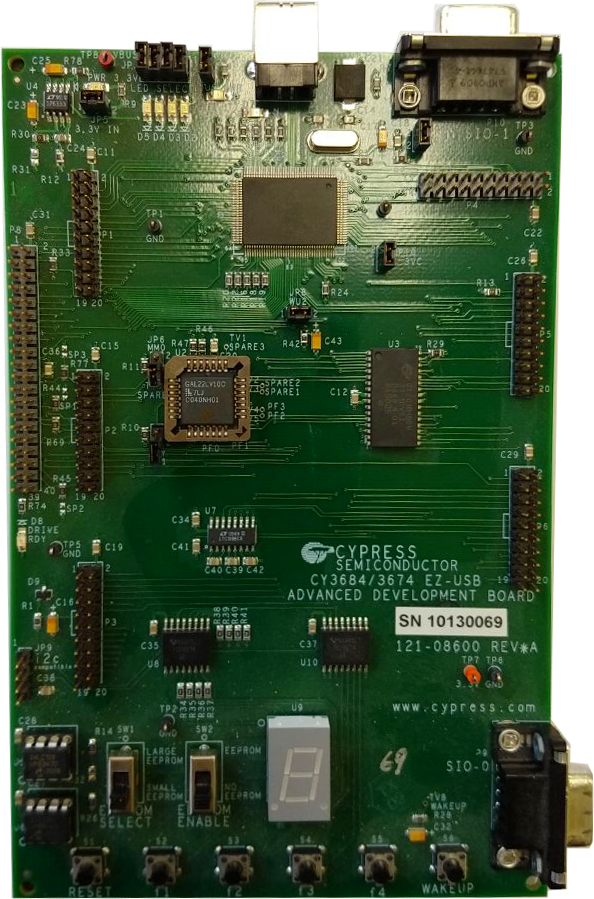
\includegraphics[width=0.4\textwidth]{32cypressboard}
\caption{Circuito impreso principal del kit de desarrollo CY3684 EZ-USB FX2LP}
\label{fig:cy3684}
\end{figure}

%En este trabajo, se utiliza el kit de desarrollo CY 3684 EZ-USB FX2LP, fabricado por Cypress Semiconductor~\cite{CypressSemiconductor2014cy3684}. El kit posee una placa de desarrollo como la que se observa en la Figura \ref{fig:cy3684}. El componente principal del kit es el controlador EZ-USB FX2LP e incorpora un display de 7 segmentos, 4 luces led multipropósito, 6 pulsadores, de los cuales 4 son de propósito general, uno de reinicio y otro que envía una señal especial para salir de un modo de bajo consumo. También tiene dos bloques de memorias EEPROM destinadas al almacenamiento del firmware (programa que ejecuta un microcontrolador), lo que otorga la posibilidad de realizar una carga no volátil de la configuración del controlador, memoria flash de \SI{64}{\kilo\byte} utilizados como RAM por el programa del controlador, un puerto USB y dos puertos UART con zócalos DE-9. Adicionalmente, cuenta con 6 puertos de 20 pines que permiten comunicarse con el controlador y 1 puerto de 40 pines, compatible con el protocolo ATA.%\\
%AQUI QUEDE

%	La arquitectura del controlador EZ-USB FX2LP se muestra en la Figura %TODO la arquitectura, pavo
%	. En ella se puede apreciar los diferentes componentes que se integran en él. Como se menciona anteriormente, la serie de circuitos integrados EZ-USB FX2LP incorporan un microcontrolador 8051, con algunas mejoras destinadas a satisfacer mejor los requerimientos del sistema USB; una interfaz serie, que permite ingresar datos uno tras otro y los entrega en forma paralela y viceversa; un transceptor USB encargado de todas las tareas de codificación y decodificación de paquetes USB; memoria RAM para programas y datos de \SI{16}{\kilo\byte}. Posee, a su vez, tres tipos de interfaces hacia periféricos externos


%	Como interfaz entre la FPGA y la PC se utilizó kit de de desarrollo CY3684 FX2LP EZ-USB Development Kit de Cypress Semiconductor,la que se observa en la Figura \ref{cy3684}. Esta placa posee como núcleo el controlador USB CY7C68013A, circuito integrado que posee todas las herramientas necesarias para realizar la interfaz, como así también un buen número de periféricos que permiten al desarrollador realizar pruebas y depuración.\\


%	Entre estas, se destacan 6 pulsadores, de los cuales cuatro se utilizan para proposito general, uno para reestablecer los valores por defecto de la placa y uno para enviar señales de suspensión y reestablecimiento del programa actualmente cargado en el microcontrolador, lo que coloca al sistema en modo bajo consumo de energía. A su vez, posee dos memorias EEPROM que sirven para cargar firmware y archivos de configuración del sistema, un display de 8 segmentos, 4 leds de multiple propósito, dos puertos UART, una salida de pines compatible con puertos ATA y 6 puertos de 20 pines que se utilizan para la conexión hacia el chip núcleo. Como soporte para el firmware, posee también un bloque con \SI{64}{\kilo\byte} de memoria SRAM.\\

%Se selecciona este controlador como interfaz ya que cuenta con una gran cantidad de herramientas que permiten realizar la comunicación USB, además de poseer memoria suficiente para datos y una interfaz de comunicación para periféricos simple lo que facilita el objetivo de utilizar la menor cantidad de los recursos configurables del FPGA, de forma tal que queden, estos últimos, disponibles para el desarrollo de otros sistemas.%\\
	
	\section{Elección de la FPGA}
		\label{mats:fpga}
		%El principal objetivo del presente Trabajo Integrador es el de proveer una comunicación USB para desarrollos basados en FPGA. Por esto mismo, es fundamental sintetizar un circuito en el FPGA que sirva de nexo entre el desarrollo y la placa de interfaz.\\

%Es por esto que se utilizó 
%Para la implementación de la comunicación de un desarrollo determinado, se requiere un nexo entre la síntesis del circuito y la memoria del controlador USB. Este vínculo se lleva a cabo mediante una pequeña MEA que ejecuta las señales de lectura y escritura. Esta MEA se desarrolla en lenguaje VHDL.\\
En la implementación de una comunicación, para poder transmitir y recibir datos, los componentes que intervienen deben seguir un protocolo establecido. Así, no solo se facilita el envío y la recepción del mensaje, sino también que determina a cada dispositivo los procedimiento que efectúa. Por este motivo, una vez definido que se utiliza una interfaz intermedia entre la PC y un FPGA (Capítulo \ref{cap:int}), y que dicha interfaz es el circuito integrado EZ-USB FX2LP de Cypress (Capítulo \ref{cap:cy}), se determina cuál es el protocolo a través del cuál se comunica cada uno de los dispositivos y se puede configurar un FPGA para que reciba y envíe datos a la interfaz.

En base a los materiales disponibles, se evaluaron tres placas de desarrollo diferentes, todas con FPGA diseñadas y comercializadas por la empresa Xilinx Inc. La placa Spartan-3E Starter, comercializada por Digilent es una placa muy potente debido a la gran cantidad de periféricos que incorpora, entre los que se destacan su pantalla LCD, los \SI{18}{\mega\byte} de memoria flash sumados a \SI{64}{\mega\byte} de SDRAM y la gran cantidad de transceptores tales como Ethernet, PS/2 para teclados y JTAG para programación y depuración.

Por su parte, la Nexys 3, tiene como núcleo un FPGA Spartan-6, es decir, un FPGA tecnológicamente superior a los FPGA Spartan-3,. El FPGA Spartan 6 brinda mayor cantidad de bloques lógicos programables, debido a que posee un método de fabricación más avanzado que permite elaborar transistores más pequeños en su circuito integrado. La miniaturización de los transistores, a su vez, otorga la posibilidad de una mayor velocidad de operación. La placa Nexis 3 también posee una gran gama de periféricos tales como pulsadores, interruptores, displays led de 7 segmentos, diferentes tipos de memorias, CODEC para comunicarse por Ethernet 10/100 o USB 2.0.

A diferencia de las anteriores, la placa de desarrollo Mojo v3 comercializada por la empresa Alchitry, es una placa de prototipado rápido. Esto quiere decir que en lugar de poseer una gran cantidad y variedaad de periféricos, se dota a la placa de una gran cantidad de puertos para que el usuario pueda colocar los perifércios que desea. Al igual que la Nexys 3, cuenta con un FPGA Spartan 6 de Xilinx. Dispone de 84 puertos digitales configurables como entrada y/o salida, 8 entradas analógicas, 8 LED's de propósito general, un botón de tipo pulsador. La principal ventaja de esta placa de desarrollo es que posee un costo notablemente inferior a las anteriores debido en gran medida a la ausencia de periféricos que, dependiendo la aplicación, pueden ser innecesarios.

Se elige para el desarrollo que se presenta en este trabajo la placa de desarrollo Mojo v3 debido a que se incorporan varios periféricos al kit CY3684 utilizado para el desarrollo de la interfaz. Además de esto, posee un FPGA superior a la placa Spartan 3E Starter, por lo que brinda la posibilidad de elaborar sistemas más complejos y veloces. En otras palabras la Mojo se selecciona por su bajo costo, versatilidad y por que está dotada por un Spartan-VI de Xilinx, que es un FPGA con una buena relación entre recursos, rendimiento, velocidad y precio.
%Existe en el mercado una amplia variedad de FPGA, como así también de placas de desarrollo que permiten desarrollar sistemas con este tipo de ciruitos integrados. El equipo de trabajo posee una placa de desarrollo Spartan-3E Starter, la cual posee como FPGA un Spartan-3 de Xilinx. Sin embargo esta placa se encuentra obsoleta, por cuanto es dificil de conseguir soporte y no es aconsejable realizar un diseño nuevo con este tipo de placas. 
%
%Por su parte el 

%Se elige para este trabajo, la placa de desarrollo MOJO v3 desarrollada por la empresa Embedded Micro. Esta placa, la cual se observa en la Figura \ref{mojo}, posee un FPGA Spartan-6 de Xilinx. El FPGA brinda la posibilidad de elaborar sistemas digitales complejos de alta velocidad y permite, al desarrollador de sensores y sistemas de adquisición de datos, la síntesis de circuitos que resuelvan problemas en la medida de los requerimientos. Dispone también de 84 puertos digitales configurables como entrada y/o salida, 8 entradas analógicas, 8 LED's de propósito general, un botón de tipo pulsador.

La Mojo v3, la cual se observa en la Figura \ref{mojo}, es una placa de desarrollo muy económica para prototipado, es decir, la fabricación de modelos funcionales. Para ello los puertos se disponen en un arreglo de pines a través de los cuales es posible acoplar el dispositivo que sea necesario. Se dispone en el mercado de otros circuitos impresos que se conectan a los pines y contienen un grupo de periféricos para propósito general. Estos circuitos impresos, se denominan shields (\textit{escudo} traducido al castellano). Se obtiene así una placa de desarrollo a la medida de las necesidades de cada proyecto. El usuario también puede diseñar sus shields o conectar las entradas y salidas de otros dispositivo mediante cables.%\\

\begin{figure}[ht]
	\centering
	\includegraphics[width = 0.4\textwidth]{mojov3}
	\caption{Placa de prototipado rápido MOJO v3, diseñada por Embedded Micro}
	\label{mojo}
\end{figure}

Además de los shields, los diseñadores pensaron en que no sea necesario ninguna herramienta extra a la hora de programar la FPGA. Para ello, dotaron al sistema de un microcontrolador ATmega32U4 de Atmel con un programa de tipo bootloader, que se encarga de transferir la configuración del FPGA (cargada desde una memoria flash incorporada, o trasmitida por el usuario desde una PC), a través de un transceptor USB que contiene el microcontrolador. Luego, el controlador es colocado en modo esclavo y se configura de forma tal que dota al sistema de una comunicación entre la FPGA y una PC, vía USB. Las entrada analógicas que posee esta placa de desarrollo también son leídas a través del microncontrolador ATmega32U4, luego de que el FPGA es programado.%\\%Luego, entra en modo esclavo, lo que permite al usuario, a posterior poder usar para debug el sistema USB que posee el microcontrolador.\\

%Una vez llegado a este punto, el lector podría preguntar con toda razón ¿por qué es necesario realizar un sistema de comunicación USB extra, si ya cuenta con un microcontrolador que se encarga de dicho asunto? La respuesta se basa en el ancho de banda del sistema de comunicación que dispone la placa.
Es importante aclarar que si bien el sistema posee alguna forma de comunicación USB utilizando el microcontrolador ATmega32U4 como interfaz, el enlace que forma posee un menor ancho de banda que el sistema en desarrollo por el presente trabajo. Esto se debe a que la línea de controladores ATmega incorpora puertos USB 2.0 full-speed. Esto quiere decir que puede enviar datos a una tasa de \SI{12}{\mega\bit\per\second}. Además, la comunicación entre ambos chips se realiza via SPI (\(Serial Peripherical Interface\), o en español Interfaz Serie de Periféricos), comandada por un cristal de cuarzo de \SI{50}{\mega\hertz}, ofreciendo una velocidad de salida que puede resultar insuficiente a los fines de este trabajo. Se pretende dotar al sistema del mayor ancho de banda posible, utilizando la capacidad de USB 2.0 High-Speed, de hasta \SI{480}{\mega bp\second}.%\\
	\section{Elección de la biblioteca libusb-1.0}
		\begin{frame}{\texttt{libusb-1.0}}
	\begin{itemize}
		\item Se utilizó la biblioteca \texttt{libusb-1.0} para la elaboración de un programa de computadoras, escrito en C, que permita leer y escribir paquetes de datos desde la PC.
		\item Esta biblioteca es de código abierto y es soportada por todos los sistemas operativos actualmente en uso. Esto brinda la reutilización del código generado.
	\end{itemize}
\end{frame}

	\section{Sumario del capítulo}
		En el presente capítulo se desarrolló y justificó la elección del controlador FX2LP como nexo entre la FPGA y la PC, brindando la conexión USB necesaria. Luego, se explicaron algunos componentes de la arquitectura implementada por Cypress a fin de proveer la comunicación USB. Finalmente, se detalló paso a paso cada uno de los componentes configurados, como así también el código desarrollado para dicho fin.

Además, se mostraron algunos detalles del framework provisto por Cypress y los encabezados necesarios para su utilización y se explicitaron los descriptores a través de los cuales se le informa al sistema las características de la comunicación que se implementa.
	
%	%for seaching files... comment to compile
%	La interfaz que este trabajo utiliza para que los datos fluyan entre un FPGA y una PC está compuesta por el controlador EZ-USB FX2LP de Cypress, el cual viene incorporado en el kit de desarrollo CY3684.

El kit de desarrollo CY3684 puede ser descompuesto en dos partes: una de hardware, que posibilita la conexión eléctrica entre los componentes y una parte de software que facilita al desarrollador tanto la elaboración del programa que es cargado en y ejecutado por el microcontrolador, denominado firmware, como las pruebas del sistema en desarrollo.

Este Capítulo aborda algunos aspectos conceptuales sobre la estructura y arquitectura del circuito integrado EZ-USB FX2LP y desarrolla
la configuración seleccionada, la elaboración del firmware y las herramientas utilizadas.%Un puerto USB posee una estructura fija: 4 contactos; dos de alimentación y dos datos. A su vez, el Protocolo USB es muy específico en cuanto a los niveles de tensión, la frecuencia de comunicación, las cadenas de bits clave que deben enviarse, entre muchas otras cosas que detalla la {Norma USB 2.0}\cite{Compaq2000}.%\\

%Un FPGA, en contraste con lo anterior, es un dispositivo electrónico que posee en su interior una gran cantidad de elemento lógicos programables. Esto permite la síntesis de casi cualquier circuito lógico. Dicha síntesis puede poseer la cantidad y disposicion de puertos como pines posea el FPGA, exceptuando algunas entradas específicas para el funcionamiento del FPGA. Esto configura una gran versatilidad que permite ajustar un sistema desarrollado dentro del FPGA a la medida necesaria.%\\

%El nexo entre los datos que se producen en sistema en el que se desenvuelve un FPGA y un puerto USB, se lo denomina interfaz. Esta última, en el presente trabajo, está compuesta por un circuito integrado particular, cuya codificación comercial es CY7C68013A, fabricado por Cypress Semiconductor. Este componente electrónico pertenece a la familia de controladores FX2LP del catálogo de integrados EZ-USB. El chip CY7C68013A se encuentra incorporado el kit de desarrollo CY3684 EZ-USB Development Kit, provisto por el fabricante.%\\

%Un kit de desarrollo es un conjunto de herramientas que permiten elaborar soluciones electrónicas que requieren un componente en particular. Además, cuenta con algunos dispositivos genéricos que posibilitan emular el sistema que utilizará el componente central del kit. En el caso del kit que se utiliza en este trabajo se descompone en dos grandes grupos: hardware y software. En la parte de hardware se incluye de un circuito impreso (PCB) que posee soldado, el integrado que nos servira de interfaz y otros componentes que se describen en el Capítulo \ref{cap:mats}.%\\

%En lo que a software se refiere, Cypress incorpora en el kit de desarrollo un código marco que posee escritas todas las funciones y registros que ejecutan las tareas que el sistema necesita para llevar a cabo la comunicación USB. Además se cuenta con herramientas de software que permite escribri, compilar y cargar el programa que se ejecuta en el controlador FX2LP.%\\

%En este capítulo se desarrolla la arquitectura de los integrados FX2LP y se abordan los módulos más relevantes para este trabajo. También se explican las herramientas del kit que fueron utilizadas para la elaboración del firmware y, finalmente, los aspectos más sobresalientes del firmware que ejecuta el CY7C68013A, y establece el funcionamiento de la comunicación USB.	
%		
%		\begin{figure}[hb]
	\centering
	\begin{tikzpicture}[scale=\textwidth/\paperwidth]
		\begin{scope}[>=latex, node distance=1, align=center, transform shape]
			\node	(aux1)	[]	{};
			\node[core,	minimum height=95]
					(mis)	[left=of aux1,anchor=north east]	{MIS};
			\node[core]	(ram)	[right=of aux1,anchor=north west, text width=30]	{16 kB RAM};
			\node[perif,text width=60]
					(xcvr)	[left=of mis]	{Transceptor USB};
			\node[interior,	minimum size=60, text width=50]
					(uc)	[above=of aux1]	{8051 Mejorado};			
			\node[perif,
			node distance=2.9]
				(pll)	[left=of uc]	{PLL};		
			\node	(aux2)	[right=of ram.south]{};				
			\node[core,	text width=120]
				(bus)	[right=of aux2,rotate=90,anchor=north west]	{Bus de datos y direcciones};		
			\node[perif]	(i2c)	[right=of bus.south east,anchor=north west]	{I2C};
			\node[perif,text width=30]
				(gpif)	[right=of bus.south west,anchor=south west] {GPIF};
			\node[perif,text width=40]
				(fifo)	[below=of gpif]	{4 kB FIFO};
			\node	(aux3)	[right=of fifo]	{};
			\node	(aux5) 	[left=of ram] {};
			\draw[<->]	(mis) -- (xcvr);
			\draw[<->]	(ram) -- (ram -| mis.east);
			\draw[<->]	(fifo) -- (fifo -| mis.east);
			\draw[<->]	(ram) to (ram -| bus.north);
			\draw[<->]	(uc) to (uc -| bus.north);
			\draw[<-]	(xcvr) to (xcvr |- pll.south);
			\draw[->]	(pll) to (uc);
			\draw[<->]	(i2c) to (i2c -| bus.south);
			\draw[<->]	(gpif) to (gpif -| bus.south);
			\draw[]		(fifo) -| (aux5.center);
		\end{scope}
	
		\begin{scope}[on background layer]
			\node[contenedor] (fx2) [fit=(pll)(xcvr)(uc)(bus)(mis)(ram)(fifo)(gpif)(i2c)(aux3)]{};
		\end{scope}
		
		\begin{scope}[transform shape,>=latex]
			\node[text width=40,align=center]	(xtal)	[left=of pll]{Xtal \SI{24}{\mega\hertz}};
			\node	(host)	[left=3of xcvr]	{PC};
			\draw[<->,ultra thick] (host) -- node [above,text width=70,midway,align=center]{Comunicación USB} (xcvr);
			\draw[->] (xtal) to (pll);
			\draw[<->,ultra thick] (bus.240) -- node [above,align=center,text width=80] {Datos, direcciones y entradas adicionales}(bus.240 -| fx2.east);
			\draw[<->,thick] (gpif) to (gpif -| fx2.east);
			\draw[<->,thick] (fifo) to (fifo -| fx2.east);
			\draw[<->,thick] (i2c) to (i2c -| fx2.east);
		\end{scope}
	\end{tikzpicture}
	%		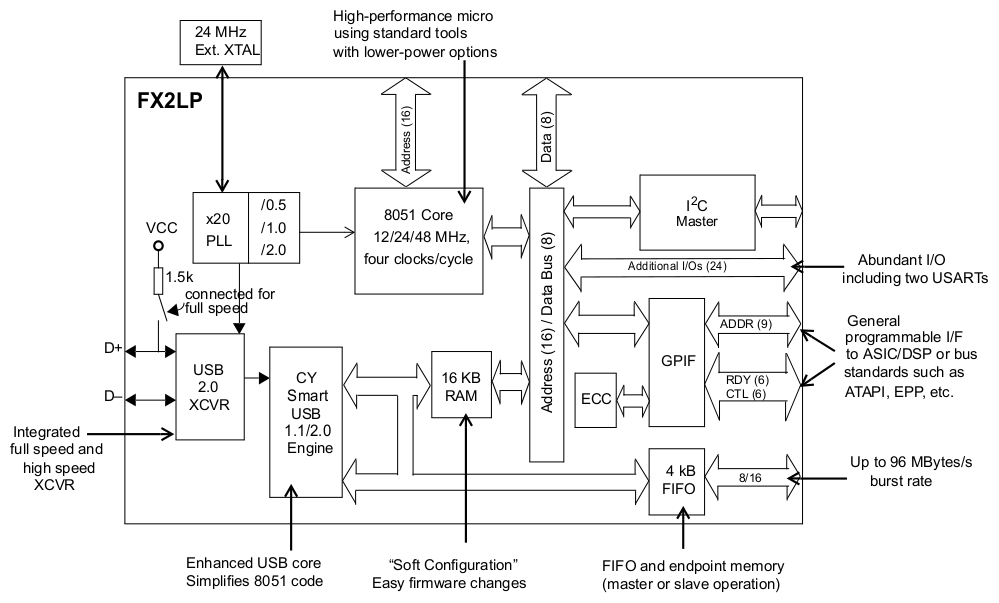
\includegraphics[width=.7\textwidth]{arqfx2lp.png}
	%		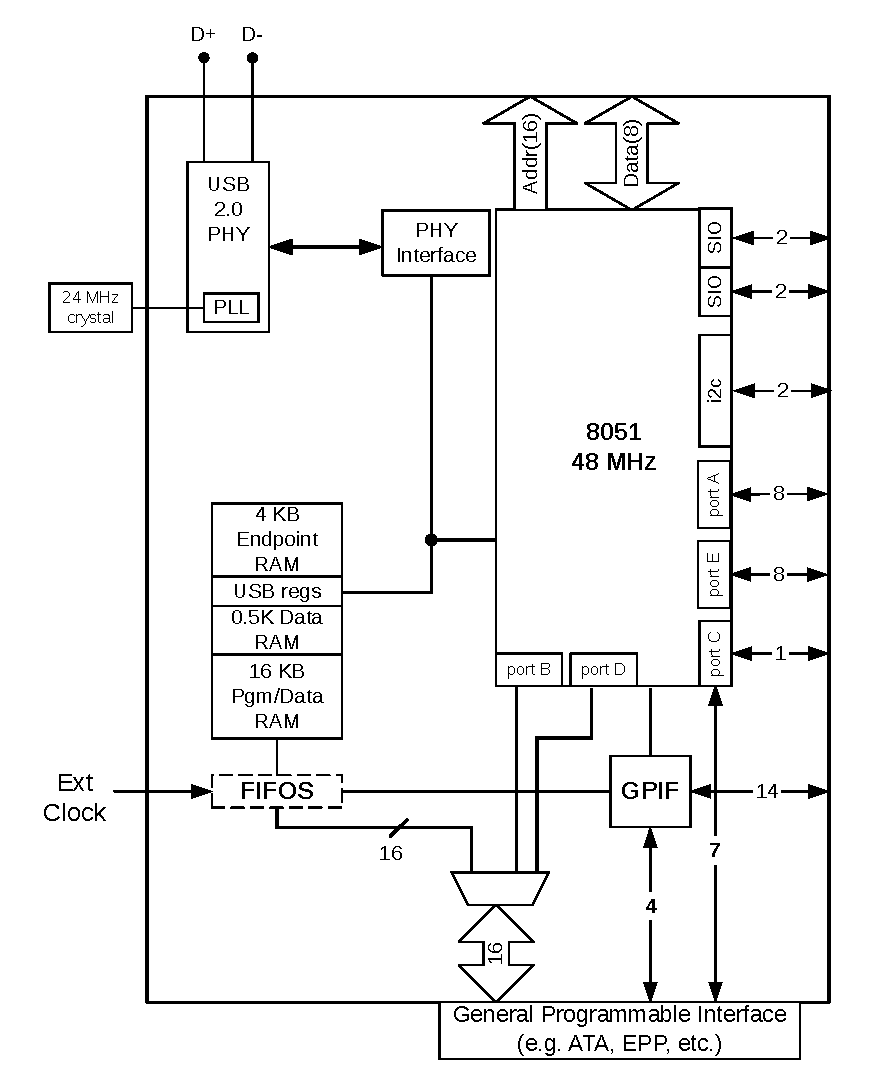
\includegraphics[width=.55\textwidth]{arq.eps}
	\caption{Arquitectura FX2LP} 
	\label{arqEzUSB}
\end{figure}

El núcleo del kit de desarrollo CY3684 es el controlador EZ-USB FX2LP. La serie de controladores FX2LP se caracteriza por brindar una conexión USB 2.0 de alta velocidad y bajo consumo energético. Está diseñada, preferentemente más no exclusivamente, para periféricos que se alimentan a baterías y poseen una autonomía energética limitada.

La arquitectura de controlador FX2LP, tal como se presenta en la Figura \ref{arqEzUSB}, integra un controlador USB completo, es decir, incluye un transceptor USB, un Motor de Interfaz Serie (MIS) y buffers configurables para datos. Incorpora también una versión del microcontrolador ($\mu$C) Intel MCS-51, más conocido como el $\mu$C 8051, que contiene registros y funciones adicionales orientadas a mejorar el rendimiento de la comunicación USB y memoria RAM de \SI{16}{\kilo\byte} de capacidad, para almacenar programas y datos. 
%Cypress agrega, como interfaz programable hacia los periféricos, una memoria tipo FIFO (\(First In First Out\); Primero Entrado, Primero Salido) con una capacidad de \SI{4}{\kilo\byte} que es operada en modo esclavo (es decir, necesita un dispositivo que le provea la lógica para operar) y destinada a almacenar datos de la comunicación, una interfaz de propósito general (GPIF) y un puerto I$^2$C. Además posee un PLL con divisor configurable a través del cual provee las señales de reloj adecuadas para el correcto funcionamiento del sistema.%\\
El modelo del flujo de datos posee dos extremos entre las cuales el controlador cumple el rol de interfaz. Estos extremos son la PC y el FPGA respectivamente. El controlador necesita, entonces, poder comunicarse tanto con el Host como con los periféricos. Para este propósito, Cypress agrega al circuito integrado del controlador dos puertos USART ((acrónimo de Transmisión y Recepción Asíncrona en Serie Universal, en inglés)), una interfaz de propósito general (GPIF), un puerto I$^2$C y una memoria FIFO (\(First In First Out\); Primero Entrado, Primero Salido).

La GPIF está pensada principalmente para poder utilizar sistemas que deban ser comandados en forma externa, como por ejemplo un registro de desplazamiento. Por su parte, la memoria FIFO posee \SI{4}{\kilo\byte} de capacidad reservados para almacenar los datos que se intercambian y se destina a aquellos sistemas que pueden proveer las señales de control, aunque también puede ser comandada por el GPIF. Con estas interfaces se posibilita la conexión con casi cualquier dispositivo, ya sea estandarizado (ATA, PCMCIA, EPP, etc) o personalizable (DSP, FPGA, $\mu$C);

%El usuario puede trasmitir datos desde y hacia el Host a través del mismo puerto USB. Sin embargo, también posee dos puertos USART ((acrónimo de Transmisión y Recepción Asíncrona en Serie Universal, en inglés)) que permiten comunicarse con la PC y facilitan en gran medida la tarea de depuración del desarrollo.

%En cuanto a la interfaz con uno o mas periféricos, el controlador posee un puerto $I^2C$, una interfaz de propósito general (GPIF), para sistemas que necesitan ser comandados en forma externa; y una interfaz con memorias FIFO esclavas, a través de las cuales se puede conectar sistemas que cumplen un rol activo en el envío y recepción de información. Estas tres interfaces posibilitan la conexión de dispositivos que poseen tanto puertos estandarizados (ATA, PCMCIA, EPP, etc.), cómo personalizables (DSP, FPGA, microcontroladores, etc).

%Variante 1
 
%El usuario puede trasmitir datos desde y hacia el anfitrión a través del mismo puerto USB, o bien via RS-232. Para comunicarse con sistemas periféricos se puede aprovechar el puerto $I^2C$, la interfaz de propósito general, que actúa como maestro y a la cual se le puede acoplar un periférico esclavo, y/o las memorias FIFO en modo esclavo que puede ser conectada a un sistema maestro. Esto brinda muchas alternativas, desde la conexión a puertos estandar, como ser ATA, PCMCIA, EPP, etc. o también la conexión de dispositivos tales como DSP's y FPGA's.\\
%\textbf{\hl{variante 1}}
%\hl{El usuario puede trasmitir datos desde y hacia el anfitrion a traves del mismo puerto USB, o bien via RS-232. Para comunicarse con sistemas perifericos se puede aprovechar el puerto $I^2C$, la interfaz de proposito general, que actua como maestro y a la cual se le puede acoplar un periferico esclavo, y/o las memorias FIFO en modo esclavo que puede ser conectada a un sistema maestro. Esto brinda muchas alternativas de conexion, desde puertos estandar, como ser ATA, PCMCIA, EPP, etc. hasta dispositivos personalizables como DSP's y FPGA's}.%\\

%variante 2
%El flujo de datos posee dos puntas entre las cuales el controlador hace de nexo. Para ello necesita poder comunicarse tanto con el \host como con los periféricos.\\
%
%El intercambio de información con el \host se lleva a cabo a través del mismo puerto USB, objetivo principal de este trabajo. Sin embargo, también posee dos puertos UART que facilitan en gran medida la tarea de depuración del desarrollo.\\
%
%En cuanto a la interfaz con uno o más periféricos, el controlador posee un puerto $I^2C$, una interfaz de propósito general (GPIF), para sistemas que necesitan ser comandados en forma externa; y una interfaz con memorias FIFO esclavas, a través de las cuales se puede conectar sistemas que cumplen un rol activo en el envío y recepción de información.\\

%\textbf{\hl{variante 2}}
%
%\hl{El flujo de datos posee dos puntas (una PC y un FPGA) entre las cuales el controlador cumple el rol de interfaz. Para ello necesita poder comunicarse tanto con el host como con los perifericos.}%\\
%
%\hl{El intercambio de informacion con el HOST se lleva a cabo a traves del mismo puerto USB, objetivo principal de este trabajo. Sin embargo, tambien posee dos puertos UART que facilitan en gran medida la tarea de depuracion del desarrollo.}%\\
%
%\hl{En cuanto a la interfaz con uno o mas perifericos, el controlador posee un puerto $I^2C$, una interfaz de proposito general (GPIF), para sistemas que necesitan ser comandados en forma externa; y una interfaz con memorias FIFO esclavas, a traves de las cuales se puede conectar sistemas que cumplen un rol activo en el envio y recepcion de informacion.}%\\

Bajo el criterio de este autor, el componente de mayor trascendencia en el funcionamiento del controlador FX2LP es el $\mu$C 8051. Es este componente el encargado de configurar los bloques programables y de inicializar todos los registros que determinan la forma en la que el sistema funciona: la frecuencia de trabajo, la gestión de las memorias y el modo en que fluyen los datos son algunas de las tareas que configura el $\mu$C. El firmware es escrito en lenguaje C para microcontroladores. 

La estructura de la interfaz implementada en este trabajo utiliza la memoria FIFO en modo esclavo, es decir, la memoria responde a señales que proporciona un maestro externo sintetizado en un FPGA. Se escogió la frecuencia de funcionamiento del PLL y se configuraron los extremos que intervienen en la comunicación USB y el modo de funcionamiento, por lo que a continuación se explicitan los detalles referidos a la configuración realizada, con lo que se busca aclarar el funcionamiento y que el lector comprenda los fundamentos de las configuraciones que se plasman en el código del firmware.

\subsection{Microcontrolador Cypress 8051 Mejorado}
	Las tareas que ejecuta el controlador FX2LP son llevadas a cabo por un microcontrolador incorporado al circuito integrado. Dicho $\mu$C es una modificación del 8051 desarrollado por Intel, para que sea más veloz en sus tiempos de ejecución y mejore el desempeño del $\mu$C cómo interfaz, mediante la incorporación de registros especiales adicionales.  De esta forma, la manera a través de la cuál el desarrollador elabora la configuración del controlador, es a través de la programación de este $\mu$C 8051.
	
	Para elaborar el firmware que ejecuta el controlador FX2LP, se desarrolló un programa en C para microcontroladores y se compiló mediante el compilador C51 de Keil, a través del entorno de desarrollo integrado Keil $\mu$Vision.
	
	Cypress provee, dentro del kit de desarrollo CY3684, un conjunto de archivos que contienen código base sobre el cual el desarrollador implementa la configuración. Este conjunto de archivos es denominado framework, el cual posee, entre otras cosas, encabezados con definiciones de macros, constantes, registros, tipos de datos y declaración de funciones prototipo. También incorpora algunas funciones precompiladas para utilizar los periféricos que contiene la placa de desarrollo.
	
	\begin{figure}[ht]
		\centering
		\begin{tikzpicture}[scale=.75\textwidth/\paperwidth]
			\begin{scope}[transform shape,node distance=1,>=latex]
				\node[mealy]	(start)	[]	{Iniciar: Reset \\ \verb|main();|};
				\node[moore]	(init)	[below=of start]	{Inicia Variables de Estado}
				edge[<-,thick] (start);
				\node[moore]	(us1)	[below=of init]		{\verb|TD_Init();|}
				edge[<-,thick]	(init);
				\node[moore]	(EI)	[below=of us1]	{Habilita\\Interrupciones}
				edge[<-,thick](us1);
				\node[node distance=0.7]			(aux1)	[below=of EI] 	{};
				\draw[<-,thick](aux1.base) to (EI);
				\node[moore,node distance=.5]	(poll)	[below=of aux1]	{\verb|TD_Poll();|}
				edge[<-,thick](aux1.base);
				\node[ask]		(pr1)	[below=of poll]	{Paquete de Setup}
				edge[<-,thick](poll);
				\node[moore]	(setup)	[right=of pr1]	{\verb|SetupComand();|};
				\draw[->,thick] (setup) |- (aux1.base);
				\node[]			(aux2)	[below=of pr1]	{};
				\draw[->,thick]	(pr1) -- node[above,near start]{Si} (setup);
				\draw[thick]	(pr1) -- node[left,near start]{No}	(aux2.base);
				\node[node distance=2.5](aux3)	[left=of aux2] {};
				\draw[thick]	(aux2.base) -- (aux3.base);
				\draw[->,thick]	(aux3.base)	|-	(aux1.base);
			\end{scope}
		\end{tikzpicture}
		\caption{Diagrama en bloques del firmware que ejecuta el $\mu$C de la interfaz}
		\label{int:fw}
	\end{figure}
	
	La Figura \ref{int:fw} muestra un diagrama de flujo del firmware que se desarrolló en el presente trabajo. El mismo se elaboró utilizando la estructura propuesta por Cypress para el desarrollo de la comunicación que se implementó. Se puede observar que al inicio del programa se inicializan variables de estado que corresponden a una máquina de estados, desarrollada por Cypress, que ejecuta las tareas de la comunicación USB.
	
	Luego, se invoca una función llamada \verb|TD_Init()|. Esta es la función a través de la cual se implementa la configuración que se desarrolló en este trabjo. En las secciones siguientes se profundiza cada uno de los bloques que intervienen.
	
	Una vez configurado el funcionamiento del controlador, se habilitan las interrupciones, lo que da lugar a que todas los bloques del circuito integrado puedan funcionar e intercambiar información. Seguidamente, el programa entra en un lazo infinito, donde en primer lugar ejecuta la función \verb|TD_Poll()|, en la cual el desarrollador programa las tareas que ejecuta el controlador durante la rutina de funcionamiento. Como segundo paso, el controlador chequea si arribó desde el Host una transferencia de control cuyo PID indique Setup. En caso afirmativo, ejecuta lo solicitado por el Host. En caso contrario, vuelve a ejecutar la función \verb|TD_Poll()|.
	
%	Keil μVision es un entorno de desarrollo integrado (IDE). Se entiende por IDE a un software
%	que integra en un entorno gráfico las herramientas que permiten elaborar un programa que
%	ejecutará un procesador, desde la escritura del algoritmo en uno o más lenguajes, su compilación,
%	las pruebas y el depurado.
%	El programa utilizado posee, entre otras cosas, editor de textos con atajos de teclado,
%	comandos que aceleran la escritura de código y resaltado de palabras claves para diferentes
%	lenguajes de programación, navegador de archivos. También ejecuta, con solo un click, el
%	compilador con la sintaxis correcta, y posee un depurador que, a través de un intérprete, permite
%	ir ejecutando el código lı́nea por lı́nea o en bloques.
%	Para realizar un programa en este entorno, Cypress provee, junto con su framework, un
%	proyecto vacı́o que puede ser copiado y pegado. Sin embargo, se puede realizar la configuración
%	manual. Las instrucciones de este procedimiento se ubican en el Apéndice ??.
%	En cuanto al compilador se refiere, el utilizado es C51. Éste es un programa que otorga
%	un archivo hexadecimal con un código que será ejecutado por microcontroladores que estén
%	implementados con la misma estructura que un Intel 8051, cómo lo es el microcontrolador que
%	posee el FX2LP.
\subsection{Frecuencia de trabajo del sistema}
	Como se menciona en la sección anterior, la configuración principal del sistema se realiza a través de la función \verb|TD_Init()|. El primer módulo configurado es el PLL ({\it Phase-Locked Loop}). Un PLL es un lazo de servocontrol cuyo parámetro controlado es la fase de una réplica, generada en forma local, de una señal de entrada\cite{Sklar2001}. En otras palabras, permite obtener dos señales iguales a través de un detector de fase. Si se incorpora un contador entre la señal generada y la entrada del comparador de fase, la señal generada tendrá una frecuencia igual al producto de la entrada por el recorrido del contador. Si, en cambio, se coloca el contador a la salida del PLL, la frecuencia puede ser dividida. Así, es posible obtener señales de frecuencia modificable.

	El PLL incorporado en el controlador permite elevar la frecuencia de un cristal de \SI{24}{\mega\hertz} hasta los \SI{480}{\mega\hertz} que necesita el transceptor USB para el cumplimiento de la norma USB. A su vez, a través de un divisor de frecuencias, permite seleccionar diferentes frecuencias de trabajo del $\mu$C 8051, entre \si{12}, \si{24} o \SI{48}{\mega\hertz}.
	
	A través de los bits especiales CLKSPD[1:0] del registro de Control y Estado de CPU (CPUCS). En la implementación realizada, se seleccionó la frecuencia de trabajo del $\mu$C a \SI{48}{\mega\hertz}.
	
	\begin{lstlisting}[language=C,backgroundcolor=\color{gray!30}]
	//CPUCS - Registro de Control y Estado del CPU
	//	CLKSPD[1:0] -> "00" => 12 MHz
	//				-> "01" => 24 MHz
	//				-> "10" => 48 MHz
	CPUCS = ((CPUCS & ~bmCLKSPD) | bmCLKSPD1); // 48 MHz
	\end{lstlisting}	

\subsection{Memoria FIFO}
	El controlador FX2LP posee una sección especial de memoria destinada al almacenamiento de los datos que fluyen desde cada uno de los extremos de la comunicación. A esta memoria pueden acceder tanto los componentes del propio controlador, como también los periféricos que desean comunicarse a través de él. Desde el punto de vista de la electrónica digital, cada uno de los componentes que acceden a esta memoria pueden tener diferentes fuentes de señal de reloj. Para salvar los inconvenientes que puede acarrear el uso de sistemas con fuentes de reloj independientes, esta porción de memoria reservada es de tipo FIFO. Debido a que se puede acceder a estas memorias FIFO tanto desde el interior de controlador FX2LP, como desde el exterior, deben ser configuradas en ambos sentidos.
	
	La memoria FIFO puede ser programada y configurada de diferentes formas, en función de los requerimientos sistemas periféricos acoplados a ella. Cada uno de los periféricos conectados a la memoria FIFO se denomina extremo o EP\footnote{EP es una abreviación del término inglés {\it endpoint}, que significa ``Extremo''. Esto quiere decir que cada uno de los periféricos conectados a la memoria FIFO es un extremo de la comunicación.}. Las características a configurar son el tamaño (\si{64}, \si{512} o \SI{1024}{\byte}), la cantidad de bloques o partes en que se divide la memoria (puede estar dividida hasta en 4 extremos) y la cantidad de buffers de datos utilizados para almacenar los datos de cada bloque de memoria.
	
	Los buffers son porciones de memoria físicamente separadas pero que, en la operación, el controlador puede intercambiar de forma tal que se acceda a ellos a través de una misma dirección de memoria. El uso de buffers múltiples implica que un EP utiliza más de un buffer. Los buffers múltiples poseen la función de evitar la congestión de datos. Con doble buffer, un periférico coloca o extrae datos del buffer de un EP, mientras el $\mu$C, utiliza otro del mismo EP. La selección del buffer donde cada componente escribe y/o lee los datos lo asigna e intercambia la interfaz en forma automática. Se pueden configurar también un triple o cuádruple buffer, lo que agrega sendas porciones de memoria extra a la reserva. De esta forma, se le otorga al sistema, en forma simultánea, gran capacidad de datos y ancho de banda.
	
	En este desarrollo, se configuró la memoria FIFO con dos EP. El EP2\footnote{EP con dirección 2.}, es un EP de entrada (envía datos al Host). Requiere una gran cantidad de datos, debido a que será por donde los sensores transmitirán todos los datos que adquieran. Además, es necesario que posea una buena cantidad de almacenamiento de datos y que estos datos sean enviados de la forma más rápida posible. Por tanto, el EP2 se configuró con dos buffers de \SI{1024}{\byte}, para que efectúe transferencias isócronas.
	
	Por su parte, se configura el EP8 como EP de salida (recibe datos desde el Host). Este EP se utiliza para recibir la configuración de los sensores, que se espera que sea de menor cantidad y más distanciada en el tiempo que los datos adquiridos. Se configuró, entonces, con dos buffers de \SI{512}{\byte} para transferencias en masa.
	
	Debido a que la memoria FIFO cumple el rol de interfaz entre los periféricos y el módulo del controlador FX2LP que efectúa las tareas propias de la comunicación USB, la configuración de dicha memoria se efectúa por separado, conteniendo información relevante a cada etapa de la comunicación.
	
\subsubsection{Interfaz hacia los periféricos}
	Cypress provee varias interfaces para comunicar el controlador hacia los periféricos. I$^2$C y UART son dos posibilidades, aunque poseen un ancho de banda muy limitado. La interfaz que opera con mayor ancho de banda es la memoria FIFO. Esta puede ser utilizadas en modo esclavo, es decir, que un sistema externo comande la lectura y la escritura de datos en ellas, o bien, a través de la interfaz GPIO, puede ser comandada por el $\mu$C 8051. La implementación que se realiza en el desarrollo de la comunicación utiliza la memoria FIFO en modo esclavo.
	
	La frecuencia de funcionamiento de estas interfaz es independiente del reloj del sistema. Puede ser configurado para usar una señal de reloj interna de \si{30} o \SI{48}{\mega\hertz}, propia de la interfaz, o bien, ser provista por un sistema externo al controlador. También, es importante indicarle al controlador si la interfaz funcionará en modo asíncrono. Todos estos parámetros son configurados a través del registro Configuración de Interfaz (IFCONFIG).
	
	La configuración que se realizó en esta implementación, utiliza el reloj interno de la interfaz, corriendo a \SI{48}{\mega\hertz}. Además, se indica que las memorias FIFO esclavas son utilizadas en modo asincrónico. Dicha configuración se plasma en las siguientes líneas de código:
	
	\begin{lstlisting}[language=C,backgroundcolor=\color{gray!30}]
	//IFCONFIG - Registro de Configuración de la Interfaz
	//	b7 	   -> fuente de reloj: '1' interna, '0' externa
	//	b6 	   -> frec: '1' 48 Mhz, '0' 30 MHz
	//	b3 	   -> asinc: '1' asíncrono
	//	b[1:0] -> modo de interfaz: "11" FIFO esclava
	IFCONFIG = 0xCB;
	SYNCDELAY;
	\end{lstlisting}

	El controlador FX2LP posee cuatro puertos que emiten señales del estado de las memorias FIFO. Estos puertos pueden ser programados para que indiquen si una porción particular de memoria se encuentra vacía, llena o si sobrepasa un nivel programable de datos. También pueden ser configurados para que indiquen el estado completo (vacío, lleno y el nivel programable) de la porción de memoria activa. Cada porción de memoria se activa a través de dos puertos de dirección, comandados por un sistema externo al controlador FX2LP.
	
	Para la comunicación desarrollada, solo son importantes las señales que indican cuando el puerto que se corresponde al EP8 está vacío y el que señala al EP2 está lleno. Si bien no son necesarias, por completitud, también se configuraron las señales EP2 vacío y EP8 lleno. Cada uno de los puertos de señal se denominan A, B, C y D y se configuran por pares a través de los registros PINFLAGSAB y PINFLAGSCD, de la forma en que se muestra a continuación.
	
	\begin{lstlisting}[language=C,backgroundcolor=\color{gray!30}]
	PINFLAGSAB = 0xBC;	// FLAGA <- EP2 Full Flag
						// FLAGD <- EP2 Empty Flag
	SYNCDELAY;
	PINFLAGSCD = 0x8F;	// FLAGC <- EP8 Full Flag
						// FLAGB <- EP8 Empty Flag
	\end{lstlisting}
	
	
\subsubsection{Interfaz hacia el módulo de comunicación USB}
	Desde el extremo interno del controlador FX2LP, la memoria FIFO se conecta al Motor de Interfaz Serial (MIS). El MIS es un módulo que se encarga de tomar datos en paralelo y convertilos en una secuencia seriada. Para cumplir con la norma USB, el MIS debe ser capaz de empaquetar, enviar, recibir y desempaquetar toda la información, así como leer los tokens que emite el host, calcular y corroborar los códigos cíclicos de detección de errores y todo lo relacionado al protocolo propiamente dicho. Luego, el transceptor USB efectúa las tareas de codificación y decodificación de los mensajes transmitidos a través del bus.
	
	Para la configuración, es necesario indicarle al controlador FX2LP el funcionamiento que tendrá cada uno de los EP. Los parámetros programables son: si está activo o no, el sentido de la comunicación (sea hacia o desde el Host), el tipo de transferencia, el tamaño de la misma y la cantidad de buffers múltiples que se utilizan. En el desarrollo que se presenta se configura el EP2 como entrada de \SI{1024}{\byte} con dos buffers y el EP8 como salida con dos buffers de \SI{512}{\byte}. También se configura el EP1 con un buffer de \SI{64}{\byte} como entrada y otro igual como salida, ya que viene implementado en una memoria separada dentro del circuito integrado FX2LP y no interfiere con el desempeño pretendido en este trabajo. Los otros EP válidos (EP4 y EP6) no se utilizan, con el objetivo de maximizar la memoria disponible para los datos útiles. De esta forma, la configuración se realiza a través de la siguiente línea de código:
	
	\begin{lstlisting}[language=C,backgroundcolor=\color{gray!30}]
	//EPxCFG - Registros de configuración de extremos
	//	b7 	   -> '1' EP activo
	//	b6 	   -> dir: '0' salida, '1' entrada
	//	b[5:4] -> tipo: "01" => isocronico
	//					"10" => masa
	//					"11" => interrupción
	//	b3 	   -> tamaño: '0' 512 bytes, '1' 1024 bytes
	//	b[1:0] -> buffer: 	"00" => x4
	//						"10" => x2
	//						"11" => x3
	EP1OUTCFG = 0xA0;
	SYNCDELAY;
	EP1INCFG = 0xA0;
	SYNCDELAY;
	// dir:entrada, tipo:isoc, tam:1024, x3
	EP2CFG = 0xDB;
	SYNCDELAY;
	EP4CFG = 0x7F; //Inactivo
	SYNCDELAY;
	EP6CFG = 0x7F; //Inactivo
	SYNCDELAY;
	// dir:salida, tipo:masa, tam:512, x2
	EP8CFG = 0xA2; 
	SYNCDELAY;
	\end{lstlisting}
	
%\subsection{Motor de Interfaz Serial}
%	El Motor de Interfaz Serial (MIS) es un módulo incorporado al circuito integrado que se encarga de tomar datos en paralelo y convertilos en una secuencia seriada.

%	\begin{figure}[ht]%TODO hacer con tikz para que quede prolija
%		\centering
%		\includegraphics[width=.8\textwidth]{usbxcvr}
%		\caption{Implementación del enlace USB realizado por el EZ-USB\cite{CypressSemiconductor2014fx2lp}}%TODO(\hl{se copiaria con tikz para mejorar prolijidad})}
%		\label{usbxcvr}
%	\end{figure}
%	
%	La comunicación USB entre el controlador FX2LP y la PC se realiza a través del transceptor, unido al MIS. Para realizar el intercambio de datos, el firmware solo debe colocar o extraer los datos de buffers programables y modificar las banderas de handshaking. En forma automática, el MIS se encargan de empaquetar, enviar, recibir y desempaquetar toda la información, así como leer los tokens que emite el host, calcular y corroborar los códigos cíclicos de detección de errores y todo lo relacionado al protocolo propiamente dicho. El transceptor codifica y decodifica todo a nivel físico.%\\
%	
%	La Figura \ref{usbxcvr} muestra la función del MIS. Toma los datos colocados en los buffers de extremos, agrega la información que corresponde al encabezado y a la cola y, finalmente, coloca el registro de handshaking. Esto último, se observan como ACK (abreviación del ingles {\it acknowledge}, que significa reconocer, aceptar o agradecer) en la Figura \ref{usbxcvr}. En el extremo del controlador, estas banderas se colocan en un registro especial que indica si el sistema está disponible, si los datos fueron colocados o leídos, dependiendo el caso tratado.

%\subsection{Modo}		
%\subsection{Buffers de extremos}
%	El MIS guarda los datos que aún no han sido enviados y/o los que han sido recibidos pero no leídos por ningún periférico en una memoria RAM específica, denominada buffer de extremo.%\\
%	
%	La norma USB define a un dispositivo extremo como una porción exclusiva e identificable de una dispositivo USB que es fuente o un sumidero de información. En otras palabras, USB ve a cada extremo como una memoria FIFO de donde surge o finaliza la información. En ingles, el termino extremo recibe el nombre de {\it endpoint}, por lo que, en adelante, cuando se hable de ellos se abreviara como EP o EPx, siendo la x un número que indica la dirección del extremo.%\\
%	
%	La serie de controladores FX2LP dispone de hasta 7 EP programables, los cuales deben poseer al menos dos buffers. La norma USB indica que cualquier dispositivo USB debe poseer un EP con dirección 0 que se destina para control y configuración, por lo que el controlador está dotado de \SI{64}{\byte} para este fin. Es el único EP que puede ser bidireccional en el sentido del flujo de datos. A través de él, host y dispositivo envían y reciben transferencias de control. Luego, se incorporan dos EP1, que poseen un buffer de \SI{64}{\byte} cada uno. Estos EP se identifican por la dirección de los datos, ya que uno de ellos es de salida y el otro de entrada de datos.%\\
%	
%	\begin{figure}[t]
%		\centering
%		\begin{tikzpicture}[scale=.7*\textwidth/\paperwidth,node distance=2.7]
%			\begin{scope}[transform shape]
%				\begin{scope}[node distance=0.4]
%					\node[buf]	(ep2b1)	[anchor=north]		{\ep{1}{2}{512}};
%					\node[buf]	(ep2b2)	[below=of ep2b1]	{\ep{2}{2}{512}};
%					\node[obuf]	(ep4b1) [below=of ep2b2]	{\ep{1}{4}{512}};
%					\node[buf]	(ep4b2) [below=of ep4b1]	{\ep{2}{4}{512}};
%					\node[obuf]	(ep6b1)	[below=of ep4b2]	{\ep{1}{6}{512}};
%					\node[buf]	(ep6b2)	[below=of ep6b1]	{\ep{2}{6}{512}};
%					\node[obuf]	(ep8b1)	[below=of ep6b2]	{\ep{1}{8}{512}};
%					\node[buf]	(ep8b2)	[below=of ep8b1]	{\ep{2}{8}{512}};
%				\end{scope}
%				
%				\begin{scope}[node distance=0.4, xshift=90]
%					\node[buf]	(ep2b3)	[anchor=north]		{\epg{1}{2}{1024}};
%					\node[obuf] (ep2b4)	[below=of ep2b3]	{\epg{2}{2}{1024}};
%					\node[obuf]	(ep2b5)	[below=of ep2b4]	{\epg{3}{2}{1024}};
%					\node[obuf]	(ep8b3)	[below=of ep2b5]	{\ep{1}{8}{512}};
%					\node[buf]	(ep8b4)	[below=of ep8b3]	{\ep{2}{8}{512}};
%				\end{scope}
%			\end{scope}
%		
%			\begin{scope}[on background layer]
%				rounded corners,]
%				\node[env, fit=(ep2b1)(ep2b2)]			(ep21)	{};
%				\node[env, fit=(ep4b1)(ep4b2)]			(ep41)	{};
%				\node[env, fit=(ep6b1)(ep6b2)]			(ep61)	{};
%				\node[env, fit=(ep8b1)(ep8b2)]			(ep81)	{};
%				\node[env, fit=(ep2b3)(ep2b4)(ep2b5)]	(ep22)	{};
%				\node[env, fit=(ep8b3)(ep8b4)]			(ep82)	{};
%				\node[draw=black,fit=(ep21)(ep82)](marco){};
%			\end{scope}
%		
%			\begin{scope}[transform shape]
%				\draw (marco.north) to (marco.south);
%				\node[left=of ep2b1.north east,anchor=north east](add1)	{0xF000};
%				\node[left=of ep2b1.south east,anchor=south east](add2)	{0xF1FF};
%				\node[left=of ep2b2.north east,anchor=north east](add3)	{0xF200};
%				\node[left=of ep4b1.north east,anchor=north east](add4)	{0xF400};
%				\node[left=of ep6b1.north east,anchor=north east](add5)	{0xF800};
%				\node[left=of ep8b1.north east,anchor=north east](add6)	{0xFC00};
%				\node[left=of ep8b2.south east,anchor=south east](add7)	{0xFFFF};
%				\draw[dashed] (add1.north west) to (add1.north west -| marco.east);
%				\draw[dashed] (add3.north west) to (add3.north west -| ep21.east);
%				\draw[dashed] (add4.north west) to (add4.north west -| marco.east);
%				\draw[dashed] (add5.north west) to (add5.north west -| marco.east);
%				\draw[dashed] (add6.north west) to (add6.north west -| marco.east);
%				\draw[dashed] (add7.south west) to (add7.south west -| marco.east);
%			\end{scope}
%	\end{tikzpicture}
%	\caption{Buffers de extremos con sus direcciones de memoria. El cuadro de la izquierda muestra la configuración por defecto. El derecho, la implementada en este trabajo.}
%	\label{epbuf}
%	\end{figure}
%	
%	Finalmente, se incorpora una memoria de \SI{4}{\kibi\byte} que debe ser configurada para los EP2, EP4, EP6 y EP8. La configuración de los EP la realiza el microcontrolador una vez que su programa se encuentra en ejecución. Las variables, conforme a los requerimientos de ancho de banda y acceso al bus son:
%	
%	\begin{itemize}
%		\item Tamaño: Dependiendo del extremo a configurar puede ser de 512 o 1024 bytes.
%		\item Tipo de acceso al bus: Definido según la norma USB, este tipo puede ser por bultos, isócrono o de interrupción. No se admiten en estos EP paquetes de control.
%		\item Cantidad de buffers: Dependiendo del extremo, puede ser dos, tres o cuatro buffers por extremo.
%		\item Habilitación: Se debe indicar al sistema si los extremos se usan o no. El EP no valido, no responderá a un pedido de entrada o salida.
%	\end{itemize}
%	
%	La Figura \ref{epbuf} muestra solo dos de las posibles configuraciones de los EP. A la izquierda se observa la configuración por defecto del controlador FX2LP. Esto es, los cuatro EP habilitados, con 512 bytes cada uno, buffers dobles y comunicación por bultos. A la derecha se muestra la configuración elegida para este trabajo, es decir, solo son EP válidos el EP2 y EP8. EP2 posee tres buffers de 1024 bytes y el EP8 dos buffers con 512 bytes de capacidad cada uno. Siempre se debe considerar que se dispone hasta \SI{4}{\kibi\byte} de memoria.%\\
%	
%	La característica de los buffers múltiples evita la congestión de datos. Con doble buffer, un periférico (o el microcontrolador) coloca o extrae datos de un buffer, mientras otro, del mismo EP, se encuentra enviando o recibiendo datos mediante el MIS. Cuando se configura un triple o cuádruple buffer, se agrega una o dos porciones mas de memoria a la reserva, respectivamente. De esta forma, se le otorga al sistema una gran capacidad de datos y ancho de banda.%\\
%	
%	Un detalle importante de los buffers múltiples es que, a la vista del controlador y/o de un periférico, el buffer posee una sola y única dirección y, es la propia interfaz FX2LP quien se encarga de seleccionar el buffer que corresponde en cada caso. Esto quiere decir que, por ejemplo, teniendo 4 buffers de \SI{512}{\byte} cada uno, el 8051 verá solo uno de \SI{512}{\byte}, sin necesidad de identificar a traves de su firmware con cuál de los cuatro está trabajando.
%	
%\subsection{Memorias FIFO esclavas}
%	\label{cy:fifo}
%	Desde el punto de vista de la electrónica digital, el MIS es un dispositivo que recibe y envía datos desde y hacia el puerto USB utilizando una señal de reloj de \SI{24}{\mega\hertz}. Esta señal, es provista por un cristal de cuarzo incorporado en el circuito impreso del Kit de Desarrollo CY3684 EZ-USB FX2LP. Por su parte, un sistema externo puede o no proveer una señal de reloj y manejo de datos propio cuy a fuente de reloj es a priori desconocida por quien configura el circuito integrado. El controlador USB incorpora memorias FIFO que se encargan de proveer una interfaz entre el MIS y un dispositivo externo, salvando el problema de poseer dos relojes diferentes e independientes.%\\
%	
%	Estas memorias funcionan en modo esclavo, es decir, se debe conectar un dispositivo capaz de proveer una lógica maestra externa que comande la entrada y salida de datos desde una memoria FIFO hacia o desde el exterior. Para los fines del presente trabajo, este modo de funcionamiento es óptimo ya que, dotando al FPGA de una máquina de estados, se logra la transferencia de datos en los tiempos requeridos.%\\
%	
%	El sistema de bus permite conectar a estas memorias hasta cuatro dispositivos diferentes. Por esto, existe un registro que permite seleccionar una porción de memoria FIFO para cada uno de los EP programables en el buffer de extremos.%\\
%	
%	\begin{figure}[ht]
%		\centering
%		\begin{tikzpicture}[scale=1*\textwidth/\paperwidth]
%			\begin{scope}[transform shape,node distance=4,>=latex]
%				\node[simple]	(fifo)		[]	 			{FIFO's Esclavas};
%				\node[simple]	(master)	[right=of fifo]	{Maestro Externo};
%				\draw[<->,thick]	([yshift=5*110/6]fifo.east) --node [above]{IFCLK} ([yshift=5*110/6]master.west);
%				\draw[<->,thick]	([yshift=4*110/6]fifo.east) --node [above]{FD[15:0]} ([yshift=4*110/6]master.west);
%				\draw[<-,thick]	([yshift=3*110/6]fifo.east) --node [above]{FIFOADR[1:0]} ([yshift=3*110/6]master.west);
%				\draw[->,thick]	([yshift=2*110/6]fifo.east) --node [above]{FLAGA} ([yshift=2*110/6]master.west);
%				\draw[->,thick]	([yshift=1*110/6]fifo.east) --node [above]{FLAGB} ([yshift=1*110/6]master.west);
%				\draw[->,thick]	([yshift=0*110/6]fifo.east) --node [above]{FLAGC} ([yshift=0*110/6]master.west);
%				\draw[->,thick]	([yshift=-1*110/6]fifo.east) --node [above]{FLAGD} ([yshift=-1*110/6]master.west);
%				\draw[<-,thick]	([yshift=-2*110/6]fifo.east) --node [above]{SLOE} ([yshift=-2*110/6]master.west);
%				\draw[<-,thick]	([yshift=-3*110/6]fifo.east) --node [above]{SLWR} ([yshift=-3*110/6]master.west);
%				\draw[<-,thick]	([yshift=-4*110/6]fifo.east) --node [above]{SLRD} ([yshift=-4*110/6]master.west);
%				\draw[<-,thick]	([yshift=-5*110/6]fifo.east) --node [above]{PKTEND} ([yshift=-5*110/6]master.west);
%			\end{scope}				
%		\end{tikzpicture}
%		\caption{Puertos de interfaz entre las FIFO's y un maestro externo}
%		\label{interfazfifo}
%	\end{figure}
%
%	La Figura \ref{interfazfifo} muestra las señales de la interfaz entre las memorias FIFO's y un maestro esclavo. Estas son:
%	
%	\begin{itemize}
%		\item IFCLK: señal de reloj. No es necesario en caso de conectar la interfaz en modo asincrónico. La señal de reloj puede ser provista por el controlador o por el dispositivo de control en forma programable.
%		\item FD[15:0]: constituye el bus de datos. Según se programe, este puede ser de 8 o 16 bits, en forma independiente para cada EP.
%		\item FIFOADDR[1:0]: puerto de direcciones. A través de él se selecciona la memoria activa en el bus.
%		\item FLAGx: Los cuatro puertos de flag son configurables e indican memoria llena, vacía o un nivel programable. También pueden indicar el estado de una memoria específica o de la que se encuentra activa a través de FIFOADDR.
%		\item SLOE, SLWR, SLRD: son las señales de control. A través de ellas el maestro entrega las ordenes de lectura y escritura.
%		\item PKTEND: a través de este puerto el maestro indica que terminó una transferencia de datos.
%	\end{itemize}

\subsection{Modos de entrada y salida automáticos}
	\begin{figure}[ht]
		\centering
		\begin{tikzpicture}[scale=0.8\textwidth/\paperwidth,text width=5em,align=center,>=latex,node distance=38mm]		
		\begin{scope}[transform shape]
		\node[interior]	(mis)									{MIS};
		\node			(im)	[right=of mis]					{};
		\node[interior]	(uc)	[above=of im]					{$\mu$C};
		\node[interior] (fifo)	[right=of im,text width=4em]	{FIFOs Esclavas};
		\node			(et)	[left=of uc]					{FX2LP};
		
		\draw[->]([xshift=1.5mm]fifo.north)to node[above,mode text]{MODO ENTRADA MANUAL} ([yshift=1mm]uc.east);
		\draw[->]([yshift=1mm]uc.west)to node[above,mode text]{MODO ENTRADA MANUAL}([xshift=-1.5mm]mis.north);
		\draw[->] ([yshift=-1mm]uc.east)to node[below,mode text]{MODO SALIDA MANUAL}([xshift=-1.5mm]fifo.north);
		\draw[->]([xshift=1.5mm]mis.north)to node[below,mode text]{MODO SALIDA MANUAL}([yshift=-1mm]uc.west);
		
		\draw[->]([yshift=1mm]fifo.west)to node[above,mode text]{MODO AUTO ENTRADA}([yshift=1mm]mis.east);
		\draw[->]([yshift=-1mm]mis.east)to node[below,mode text]{MODO AUTO SALIDA}([yshift=-1mm]fifo.west);
		
		\node[exterior]	(pc)	[left=of mis]	{Host};
		\draw[->]([yshift=1mm]mis.west)to([yshift=1mm]pc.east);
		\draw[->]([yshift=-1mm]pc.east)to([yshift=-1mm]mis.west);
		
		\node[exterior]	(fpga)	[right=of fifo]	{Maestro Externo};
		\draw[->]([yshift=1mm]fifo.east)to node[above]{Banderas}([yshift=1mm]fpga.west);
		\draw[<-]([yshift=-1mm]fifo.east)to node[below]{Control}([yshift=-1mm]fpga.west);
		\end{scope}	
		
		\begin{scope}[on background layer]
		\node(fx)[rounded corners,fill=black!10,fit=(mis)(uc)(fifo)(et)]{};
		\end{scope}
		\end{tikzpicture}
		\caption{Modos de conexión de la memoria FIFO, el microntrolador y el MIS}
		\label{modesfifo}
	\end{figure}

	
	Los datos se reciben o envían a través del MIS. Dichos datos, pueden ser enviados en forma automática desde y hacia las memorias FIFO, o bien, pueden ser dirigidos hacia el $\mu$C, el cual debe dirigir los datos desde y hacia su destino (el MIS o las memorias). Esto último permite leer, modificar, suprimir, agregar y/o generar nuevos datos antes de ser remitidos a su destinatario. Estos caminos se pueden ver en la Figura \ref{modesfifo}.%\\
	
	Aunque el envío de datos se hace siempre sin intervención de una persona, el fabricante llama a estos caminos "MODO MANUAL", en caso de enviar los datos a través del $\mu$C 8051, y "MODO AUTOMÁTICO", cuando la comunicación es directa entre el MIS y las FIFO. Además, se programan en forma independiente para cada extremo, sea este de salida o entrada. Es decir, la entrada de un EP puede ser manual y la entrada de otro puede ser automática.%\\
	
	Se debe notar en la Figura \ref{modesfifo} que se refiere a paquetes de entrada cuando estos poseen una dirección que se inicia en un periférico y termina en el host y de salida cuando llevan el sentido contrario. Esto se debe al rol central que ejerce el host en la comunicación USB.
	
	Para efectuar la configuración del modo de funcionamiento de cada EP, se recurre a los Registros de Configuración Extremo-FIFO esclava (EPxFIFOCFG). A continuación se muestra la programación efectuada en este trabajo, en donde se envían los datos en forma automática, tanto de entrada como de salida. Se debe notar que la activación del modo automático se produce por el flanco ascendente de la variable de configuración, por lo que primero se coloca el registro en cero y luego se establece el valor de la configuración. También se indica en este registro que los datos tendrán un ancho de 16 bits.
	
	\begin{lstlisting}[language=C,backgroundcolor=\color{gray!30}]
	//EPxFIFOCFG - Registro de configuracion extremo/FIFO
	//	b6	->	'1' Indica lleno un byte antes
	//	b5	->	'1' Indica vacío un byte antes
	//	b4	->	'1' Modo Auto Salida
	//	b3	->	'1' Modo Auto Entrada
	//	b2	->	'1' Permite paquetes de entrada con largo 0
	//	b0	->	'1' bus de 16 bits, '0' bus de 8 bits
	EP8FIFOCFG = 0x00;
	SYNCDELAY;
	EP2FIFOCFG = 0x00;
	SYNCDELAY;
	
	//establecer modo auto. se necesita flanco ascendente
	EP8FIFOCFG = 0x11;
	SYNCDELAY;
	EP2FIFOCFG = 0x0D;
	SYNCDELAY;
	\end{lstlisting}
	
	Una vez configuradas las interfaces, se deben restablecer las memorias FIFO, a fin de asegurarse que se encuentran vacías para iniciar la comunicación, a través del registro FIFORESET. El bit 7 de este registro le indica al MIS que la memoria FIFO no se encuentra disponible, y el MIS, a su vez, lo indica al Host si es necesario. Luego, a través de los cuatro bits menores se indica la dirección del EP a restablecer. Finalmente, libera la memoria y se le indica la situación al MIS.
	
	\begin{lstlisting}[language=C,backgroundcolor=\color{gray!30}]
	//FIFORESET - Registro de restablecimiento FIFO
	//	b8		->	'1' Desabilitado
	//	b[3:0]	->	'1' Direccfión de EP
	FIFORESET = 0x80;
	SYNCDELAY;
	FIFORESET = 0x82;
	SYNCDELAY;
	FIFORESET = 0x84;
	SYNCDELAY;
	FIFORESET = 0x86;
	SYNCDELAY;
	FIFORESET = 0x88;
	SYNCDELAY;
	FIFORESET = 0x00;
	SYNCDELAY;
	//establecer modo auto. se necesita flanco ascendente
	EP8FIFOCFG = 0x11;
	SYNCDELAY;
	EP2FIFOCFG = 0x0D;
	SYNCDELAY;
	\end{lstlisting}
	

	En las líneas de código mostradas hasta acá se utiliza el macro {\it SYNCDELAY;}. Dicho macro es una secuencia de espera requerida por Cypress para cumplir con los tiempos de mantenimiento asociados a la escritura y lectura de determinados registros\cite{CypressSemiconductor2014fx2lp}.%, los cuales se explicitan en el Anexo \ref{an:syncdelay}.

		
	\chapter{Pruebas de funcionamiento y desempeño del sistema desarrollado}
	\label{cap:verif}
	La interfaz que este trabajo utiliza para que los datos fluyan entre un FPGA y una PC está compuesta por el controlador EZ-USB FX2LP de Cypress, el cual viene incorporado en el kit de desarrollo CY3684.

El kit de desarrollo CY3684 puede ser descompuesto en dos partes: una de hardware, que posibilita la conexión eléctrica entre los componentes y una parte de software que facilita al desarrollador tanto la elaboración del programa que es cargado en y ejecutado por el microcontrolador, denominado firmware, como las pruebas del sistema en desarrollo.

Este Capítulo aborda algunos aspectos conceptuales sobre la estructura y arquitectura del circuito integrado EZ-USB FX2LP y desarrolla
la configuración seleccionada, la elaboración del firmware y las herramientas utilizadas.%Un puerto USB posee una estructura fija: 4 contactos; dos de alimentación y dos datos. A su vez, el Protocolo USB es muy específico en cuanto a los niveles de tensión, la frecuencia de comunicación, las cadenas de bits clave que deben enviarse, entre muchas otras cosas que detalla la {Norma USB 2.0}\cite{Compaq2000}.%\\

%Un FPGA, en contraste con lo anterior, es un dispositivo electrónico que posee en su interior una gran cantidad de elemento lógicos programables. Esto permite la síntesis de casi cualquier circuito lógico. Dicha síntesis puede poseer la cantidad y disposicion de puertos como pines posea el FPGA, exceptuando algunas entradas específicas para el funcionamiento del FPGA. Esto configura una gran versatilidad que permite ajustar un sistema desarrollado dentro del FPGA a la medida necesaria.%\\

%El nexo entre los datos que se producen en sistema en el que se desenvuelve un FPGA y un puerto USB, se lo denomina interfaz. Esta última, en el presente trabajo, está compuesta por un circuito integrado particular, cuya codificación comercial es CY7C68013A, fabricado por Cypress Semiconductor. Este componente electrónico pertenece a la familia de controladores FX2LP del catálogo de integrados EZ-USB. El chip CY7C68013A se encuentra incorporado el kit de desarrollo CY3684 EZ-USB Development Kit, provisto por el fabricante.%\\

%Un kit de desarrollo es un conjunto de herramientas que permiten elaborar soluciones electrónicas que requieren un componente en particular. Además, cuenta con algunos dispositivos genéricos que posibilitan emular el sistema que utilizará el componente central del kit. En el caso del kit que se utiliza en este trabajo se descompone en dos grandes grupos: hardware y software. En la parte de hardware se incluye de un circuito impreso (PCB) que posee soldado, el integrado que nos servira de interfaz y otros componentes que se describen en el Capítulo \ref{cap:mats}.%\\

%En lo que a software se refiere, Cypress incorpora en el kit de desarrollo un código marco que posee escritas todas las funciones y registros que ejecutan las tareas que el sistema necesita para llevar a cabo la comunicación USB. Además se cuenta con herramientas de software que permite escribri, compilar y cargar el programa que se ejecuta en el controlador FX2LP.%\\

%En este capítulo se desarrolla la arquitectura de los integrados FX2LP y se abordan los módulos más relevantes para este trabajo. También se explican las herramientas del kit que fueron utilizadas para la elaboración del firmware y, finalmente, los aspectos más sobresalientes del firmware que ejecuta el CY7C68013A, y establece el funcionamiento de la comunicación USB.
	\section{Depuración de la configuración de la interfaz FX2LP}
		%Durante el desarrollo de este trabajo, se halló un problema importante sobre la compilación y ejecución del código escrito en C para microcontroladores. Dicho problema consiste en 

%Durante el desarrollo del código precedentemente explicado, 
Se realizaron diversas pruebas y versiones tanto para resolver problemas como para verificar el correcto funcionamiento de la interfaz.

El primer problema que se presentó fue una inestabilidad en la ejecución del código, la cual se mostraba en forma intermitente al cargar el código compilado. La inestabilidad hacía que el código repentinamente se detuviera en la ejecución de la inicialización del dispositivo. A fin de salvar dicho problema, se recurrió al envío de mensajes de seguimiento a través de los puertos UART que prevee el controlador FX2LP.

También se realizaron pruebas de robustez en la comunicación, pudiendo enviar y recibir datos por el mismo puerto UART, aprovechando la configuración establecida. Para la recepcion de datos en la PC se utilizó el programa Hercules\cite{HWGroup}. Dicho programa es una desarrollo cuya descarga es libre y permite configurar y recibir mensajes a través de diferentes puertos.

Como testigo del funcionamiento de los flags, se asociaron sus valores a los LED de propósito general, de forma tal que se pueda corroborar que los endpoint usados recibian y enviaban los datos cuando se emitía la orden desde el Host.

\subsection{Biblioteca FX2LPSerial}
Para la configuración y utilización del puerto UART 0 se recurrió a la biblioteca FX2LPSerial\cite{Kumar2017}. Esta biblioteca es un conjunto de funciones de C para microcontroladores que resuelven la configuración los puertos UART y de las rutinas asociada a la recepción y envío de datos por dichos puertos. 

La configuración del puerto UART se realizó a través de la función \verb|FX2LPSerial_Init()|. Esta función configura los registros de los contadores para establecer una tasa de transmión de 38400 baudios. Luego, asegura que el reloj que utiliza el puerto UART se encuentre configurado. Esto se realiza a través del Registro de Configuración de la Interfaz (IFCONFIG), el cual se setea para correr a \SI{48}{\mega\hertz}, la misma a la cual funciona el sistema desarrollado, por lo que no presenta problemas de compatibilidad. Si bien es posible cambiar la velocidad de transmisión, esta configuración posee una desviación del 0,16\%\cite{CypressSemiconductor2014fx2lp} entre la tasa nominal y la tasa real de transferencia. Esta diferencia de tasas es suficiente para asegurar que funcione en cualquier dispositivo. Por lo tanto, se decidió utilizar la configuración con los valores por defecto.

%Durante la compilación y ejecución de las tareas provista por Cyress a traves de su framework, sucedió que de forma inesperada, el controldaor FX2LP no lograra inicializar en forma correcta su funcionamiento. Se dice que sucedía en forma inesperada ya que no había causa aparente para este comportamiento anómalo: el compilador no informaba error alguno y el código desarrollado no tenía nada de malo luego de diversa revisiones.

%Para verificar el código desarrollado, se utilizó un programa monitor precompilado, el cual es provisto por Cypress. Este monitor permite al desarrollador acceder a operaciones de depuración, tales como el chequeo de variables, el pausado y reanudado de ejecuciones, etc. El desarrollo realizado funcionó sin inconvenientes a través de este monitor.

%Luego, se buscó correr el programa con alguna función que permitiese seguir la ejecución de la rutina implementada. Para ello, se utilizó la biblioteca FX2LPSerial\cite{Kumar2017}. Esta biblioteca es un conjunto de funciones de C para microcontroladores que se sirven para configurar los puertos UART y de las rutinas asociada a la recepción y envío de datos por dichos puertos. Así, se configuró el envió de mensajes por UART y que luego se recibieron en una PC.

%La configuración del puerto UART se realizó a través de la función \verb|FX2LPSerial_Init()|. Esta función configura los registros de los contadores para establecer una tasa de transmión de 38400 baudios. Luego, asegura que el reloj que utiliza el puerto UART se encuentre configurado. Esto se realiza a través del Registro de Configuración de la Interfaz (IFCONFIG), el cual se setea para correr a \SI{48}{\mega\hertz}, la misma a la cual funciona el sistema desarrollado, por lo que no presenta problemas de compatibilidad.Si bien es posible cambiar la velocidad de transmisión, esta configuración posee un diferencia del 0,16\%\cite{CypressSemiconductor2014fx2lp}, lo que asegura que funcione en cualquier dispositivo, por lo tanto, se decidió dejarla tal cual está.

Para la recepcion de datos en la PC se utilizó el programa Hercules\cite{HWGroup}. Dicho programa es de descarga libre y permite configurar y recibir mensajes a través de protocolo Ethernet o por puerto Serie. Se configuró el puerto UART, en la pestaña destinada al monitoreo del puerto Serie, con una tasa de transmisión de 38400 baudios, 8 bit, sin paridad y sin handshaking. A través de esta configuración recibie cualquier dato enviado a través de los puertos UART del controlador FX2PL y los muestra en formato ASCII.

Una vez configurado el envío de datos a través del puerto UART, se procedió a enviar mensajes de control para poder corroborar la funcionalidad y comprobar si efectivamente el controlador efectuaba sus tareas y en que momento dejaba de hacerlo.

Se pudo determinar que en la función \verb|main()|, luego de realizar la inicialización de todos los modulos, procede a la desconexión del controlador con el puerto USB, a través de una rutina que Cypress denomina ReNumertion\cite{CypressSemiconductor2014fx2lp}. Durante la reconexión ocurre algún efecto, aún no identificado, que hace que el programa se detenga cuando debe reconectarse. Este desperfecto fue solucionado con el agregado de una línea de comunicación después de el activado del reconcetado. Esto demostró ser lo suficientemente robusto ya que eliminando todas las  líneas que envían datos de monitoreo no aparació nuevamente la detención del programa, más sí, eliminando solo esa línea de código. De esta manera, el código queda de la siguiente forma en donde la línea 190 es la agregada en este trabajo:

\begin{lstlisting}[language=C,backgroundcolor=\color{gray!30},numbers=left,firstnumber=189,basicstyle=\footnotesize]
	 USBCS &=~bmDISCON;
	 FX2LPSerial_XmitString("Reconectando...\n\n");
\end{lstlisting}

\subsection{Testigos LED}
Los LED multipropósito incorporados en la placa de desarrollo CY3684, fueron programados para que repliquen el estado de los flags de vaciado y de llenado de los EP. De esta forma, se pudo monitorear la carga de datos en el controlador y la descarga a través del puerto USB y vicersa.

Los LED se encuentran conectados a través de un decodificador. Para su encendido, es necesario la lectura de las direcciones hexadecimales de memoria 80xx, 90xx, A0xx y B0xx, mientras que para su apagado, las direcciones a leer son  88xx, 98xx, A8xx y B8xx\cite{CypressSemiconductor2014cy3648}. Por ello, se elaboró el encabezado {\it leds.h}, el que se observa a continuación.
	
	\begin{lstlisting}[language=C,backgroundcolor=\color{gray!30}]
	xdata volatile const BYTE D2ON	_at_ 0x8800;
	xdata volatile const BYTE D2OFF	_at_ 0x8000;
	xdata volatile const BYTE D3ON	_at_ 0x9800;
	xdata volatile const BYTE D3OFF	_at_ 0x9000;
	xdata volatile const BYTE D4ON	_at_ 0xA800;
	xdata volatile const BYTE D4OFF	_at_ 0xA000;
	xdata volatile const BYTE D5ON	_at_ 0xB800;
	xdata volatile const BYTE D5OFF	_at_ 0xB000;	\end{lstlisting}
	
Luego, con el propósito de enceder o apagar los diodos emisores de luz, es necesario declarar una variable auxiliar y asignarle los punteros declarados. Así, a través de la función \verb|TD_Poll()|, que es la función que se ejecuta en el loop infinito del controlodaro FX2LP, se colocó la el siguiente código:

	\begin{lstlisting}[language=C,backgroundcolor=\color{gray!30}]
void TD_Poll(void)             // Called repeatedly while the device is idle  
{
	BYTE dum;
	
	if(EP8FIFOFLGS & bmBIT1)//ep8 fifo empty
	{
		dum = D4ON;
	}
	else
	{
		dum = D4OFF;
	}

	if(EP8FIFOFLGS & bmBIT0)//ep8 fifo full
	{
		dum = D3ON;
	}
	else
	{
		dum = D3OFF;
	}
	if(EP2FIFOFLGS & bmBIT1)//ep2 fifo empty
	{
		dum = D2ON;
	}
	else
	{
		dum = D2OFF;
	}
}
	\end{lstlisting}

A través de los registros EPxFIFOFLGS se puede conocer el estado de cada uno. Aplicando una máscara bit a bit, se obtiene el estado de cada uno de los flags. Así, dependiendo del estado de cada uno de ellos, se enciende o se apagan las luces.
Esta rutina resultó de mucha utilidad a la hora de realizar las diferentes pruebas, tanto del funcionamiento de la interfaz, como de la conexión entre la itnterfaz y el FPGA.

\subsection{Prueba de envío y recepcion de datos}
	Para la verificación de la conexión entre la PC y la interfaz, a través del protocolo USB, se utilizó el programa {\it Cypress USB Control Center}, provisto por Cypress dentro del kit de desarrollo CY3684, con el cual se desarrolló este trabajo. Dicho software permite cagar el firmware desarrollado en la interfaz y, a su vez, detalla la información recibida a través de los descriptores y posibilita el envío y recepción de mensajes.
	
	Para corroborar que el envío de datos fue existoso, se procedió a enviar datos a través del {\it Cypress USB Control Center}. Así, en primer lugar, corroborando que el LED que indica que el EP8 se encuentra vacío se apaga, se infirió que los datos estaban llegando. A continuación, se enviaron más datos hasta lograr que el LED asociado al límite de capacidad del EP8 se encendiese. Luego, a través de un pulsador, se activa una rutina de envío de los datos guardados en el EP8 a través del puerto UART. Para ello, fue necesario realizar unos pequeños ajustes en la configuración.
	
	El controlador FX2LP de Cypress permite manipular los datos de los paquetes USB. Sin embargo, la configuración por defecto, no permite realizar esta tarea. Para ello es necesario, en primer lugar, desactivar lo que Cypress llama el armado automático de paquetes y habilitar la manipulación avanzada de paquetes\cite{CypressSemiconductor2014fx2lp}.
	
	A medida que los datos van ingresando al controlador FX2LP a través del puerto USB, el Motor de Interfaz Serial (MIS) los coloca en el espacio de memoria asignado y va incrementando un contador por cada byte recibido. De esta forma, la interfaz puede saber cuantos datos, efectivamente, posee almacenados. Sin embargo, cuando los datos ingresan a través de la memoria FIFO, es otro el contador incrementado. El armado automático de paquetes realiza la tarea de emparejar estos contadores, de forma tal que no se deba destinar tiempo de ejecución de $\mu$C para esta tarea.
	
	Para poder escribir datos en la memoria y informarle al MIS que se agregaron datos, es necesario que este armado autmático está desactivado. Esto implica que cuando lleguen datos, el controlador debe poder realizar esta operación. A su vez, por defecto los paquetes que llegan desde la PC no pueden ser modificados. Para realizar esto, es necesario hablitar el manejo mejorado de paquetes. Tanto la manipulación avanzada de paquetes como el armado automático se encuentran los dos bits menos significativos del Registro de Control de Revisión (REVCTL).
	
	Una vez activados ambos bits del registro REVCTL, se debe efectuar la rutina que armará los paquetes en forma ``manual''. Para este propósito, se activó una interrupción que se dispara cada vez que llegan mensajes a un EP determinado, en este caso, el EP8. Toda esta configuración se realizó en las últimas líneas de la función \verb|TV_Init()|, la cual quedó de la siguiente forma:
	
	\begin{lstlisting}[language=C,backgroundcolor={gray!30}]
	
	\end{lstlisting}
	%Uso de Interrupciones
	%Uso de pulsasdores
	%Sobre RevCtl 
	\section{Pruebas de la síntesis de la MEF en el FPGA}
		%INTENTO 1

%En el Capítulo \ref{cap:int} se detalló que el sisetma desarrollado se compone de tres componentes principales, a saber: El Host, cuyo rol es llevado a cabo por una PC; la interfaz, integrada por el controlador FX2LP de Cypress y un FPGA, en este caso un Spartan-6 de Xilinx. A su vez, el Capítulo \ref{cap:fpga}, indica que el sistema interno del FPGA lleva una Maquina de Estados Finitos (MEF), cuya función es la de realizar el efectivo intercambio de datos con la interfaz, y un sistema genérico.
%
%Hasta acá se ha desarrollado la configuración de la interfaz y la implementación de la MEF. Sin embargo, es necesario, que el sistema pueda funcionar en forma autónoma, proveerle un sistema mínimo que pueda hacer las veces de fuente y sumidero de datos. Es por esto, que se dotó al sistema con una memoria FIFO con el objetivo de implementar un eco que permita realizar una evaluación de desempeño de la comunicación desarrollada. Así, se permite enviar mensajes desde una PC y que estos sean recibidos luego.
%
%\subsection{Implementación de la memoria FIFO en el FPGA}
%	La memoria FIFO sintetizada en el FPGA se obtuvo a través de la herramienta {\it Core Generator} provista por Xilinx junto con el entorno de desarrollo ISE, utilizado en este trabajo para el desarrollo\cite{XilinxInc}. La configruación seleccionada generó una memoria FIFO de 511 bytes, con puertos de entrada y salida dedicados, es decir uno de entrada y uno de salida, un bus de 16 bits de ancho. Posee señal de reconocimiento de escritura. También se dotó a la memoria generada con entradas de reloj y habilitación de bus independientes tanto para el puerto de entrada como el puerto de salida.
%	
%	
%INTENTO 2
%TODO debería decir como generar cada una de las señales internas propuesas en el capitulo correspondiente... la magen en cuestion es \ref{fpga:intersignal}
Con el objetivo de verificar el sistema desarrollado, se procedió a implementarlo en un sistema mínimo que sea capaz de utilizar la comunicación, de forma tal que el Host pueda establecer un enlace con el FPGA. Para ello, se implementó un sistema eco, es decir, un sistema que recibe los mensajes que envía el Host y, luego, los transmite para que el Host pueda recibirlos. De esta forma, el Host puede reconocer que los datos enviados no fueron perdidos ni modificados.

\begin{figure}[ht]
	\centering
	\begin{tikzpicture}[scale=.7]
		\begin{scope}[transform shape,node distance=4,>=latex,double distance=1.3]
			\node[simple](fx2lp){Interfaz FX2LP};
			
			\node[simple, rounded corners,minimum size=80] (PC)[left=2 of fx2lp]{PC};
			\draw[double,<->](PC) -- node[above]{USB} (fx2lp);
			
			\node[simple](mea)[right=of fx2lp]{Maquina de Estados Algorítmica};
			
			\draw[double,<->] ([yshift=3.5*110/4]fx2lp.east)-- node [above]{FDATA[15:0]} ([yshift=3.5*110/4]mea.west);
			\draw[double,<->] ([yshift=2.5*110/4]fx2lp.east)-- node [above]{FADDR[1:0]} ([yshift=2.5*110/4]mea.west);
			\draw[->] ([yshift=1.5*110/4]fx2lp.east)--node[above]{FLAG\_Vacío} ([yshift=1.5*110/4]mea.west);
			\draw[->]([yshift=.5*110/4]fx2lp.east)--node[above]{FLAG\_Lleno}([yshift=.5*110/4]mea.west);
			\draw[<-]([yshift=-.5*110/4]fx2lp.east)--node[above]{SLOE}([yshift=-.5*110/4]mea.west);
			\draw[<-]([yshift=-1.5*110/4]fx2lp.east)--node[above]{SLRD}([yshift=-1.5*110/4]mea.west);
			\draw[<-]([yshift=-2.5*110/4]fx2lp.east)--node[above]{SLWR}([yshift=-2.5*110/4]mea.west);
			\draw[<-]([yshift=-3.5*110/4]fx2lp.east)--node[above]{PKTEND}([yshift=-3.5*110/4]mea.west);
			
			\node[simple,minimum size=50](clk)[right=of mea.south east,anchor=south west] {PLL};
			\draw[<-]([]mea.east |- clk.west)--node[above]{Reloj}([]clk.west);
%			\draw[<-]([yshift=-1*80/3]mea.north east)--node[above]{Reloj}([yshift=-1*80/3]clk.north west);
%			\draw[<-]([yshift=-2*80/3]mea.north east)--node[above]{Reset}([yshift=-2*80/3]clk.north west);
			\node[rounded corners,simple, minimum size=50](clkSrc)[below=1 of clk]{Fuente de reloj};
			\draw[->](clkSrc) to (clk);
			
			\node[simple,minimum height=150,minimum width=50](interno)[right=of mea.north east,anchor=north west]{Memoria FIFO};
			\draw[double,->]([yshift=-.5*150/6]mea.north east)--node[above]{Dato\_enviado[15:0]} ([yshift=-.5*150/6]interno.north west);
			\draw[double,<-]([yshift=-1.5*150/6]mea.north east)--node[above]{Dato\_a\_enviar[15:0]}([yshift=-1.5*150/6]interno.north west);
			\draw[<-]([yshift=-2.5*150/6]mea.north east)--node[above]{Enviar\_datos}([yshift=-2.5*150/6]interno.north west);
			\draw[->]([yshift=-3.5*150/6]mea.north east)--node[above]{SLRD}([yshift=-3.5*150/6]interno.north west);
			\draw[->]([yshift=-4.5*150/6]mea.north east)--node[above]{SLWR}([yshift=-4.5*150/6]interno.north west);
			\draw[<-]([yshift=-5.5*150/6]mea.north east)--node[above]{PKTEND}([yshift=-5.5*150/6]interno.north west);
			
		\end{scope}
		\begin{scope}[]
			\node[rounded corners,inner ysep=5pt,draw=black,rectangle,fit={(mea)(interno)},label=north:FPGA](fpga){};
			\node[inner ysep=11pt, yshift= 8pt, draw=black,rectangle,fit={(fpga)(clkSrc)},label=north:Mojo](){};
		\end{scope}
	\end{tikzpicture}
	\caption{Diagrama en bloques del sistema de prueba}
	\label{test:sist}
\end{figure}

Para establecer un sistema eco, se deben implementar todas las señales de control que se observan en la Figura \ref{fpga:intersignal}. Estas son, señal de reset, señal de reloj, solicitud  sde envío de datos y los datos a enviar. A su vez, se deben poder leer los datos recibidos y las señales {\it SLWR} y {\it SLRD}, a través de las cuales el sistema señala el cambio de dato. 

Con el objetivo de poder recibir, almacear y reenviar los datos que llegan desde la interfaz, se sintetizó en el FPGA una memoria FIFO que almacene los datos y, cuando el EP de salida no posee más datos, es decir que el {\it Flag Vacío} se encuentra activo, retransmita los datos hacia la interfaz hasta que el Host los solicite.

Una vez incorporados los componentes al FPGA, se realizó su validación funcional antes de ser cargado todo el desarrollo al FPGA para efectuar las pruebas del sistema. A continuación, se detallarán los componentes y señales que se sintetizaron, como así también la verificación realizada.

\subsection{Declaración de la entidad}
	Para la implementación y síntesis del sistema, es necesario declarar los puertos que tendrán una correspondencia física con un pin de salida del FPGA en la descripción de mayor jerarquía. El archivo que posee una mayor jerarquía es usualmente llamada top.
	
	Como se conoce cuáles son las señales a través de las cuales el FPGA debe conectarse con la interfaz, es posible declarar la entidad que se sintetizó. Además se declararó  la señal de reloj, que proviene desde la placa Mojo v3. El código de descripción en donde se declaró la entidad se muestra a continuación.
	
	\begin{lstlisting}[language=VHDL,backgroundcolor=\color{gray!30}]
entity fx2lp_interface_top is
	generic(
		constant in_ep_addr:	std_logic_vector(1 downto 0) := "00";
		constant out_ep_addr:	std_logic_vector(1 downto 0) := "11";
		constant port_width: integer := 16
		);
	port(
		fdata   : inout std_logic_vector(port_width-1 downto 0);  
		faddr   : out   std_logic_vector(1 downto 0);
		slrd    : out   std_logic;
		slwr    : out   std_logic;
		flaga   : in    std_logic;
		flagb   : in    std_logic;
		flagc   : in    std_logic;
		flagd   : in    std_logic;
		sloe    : out   std_logic;
		pktend  : out   std_logic;
		clk_in  : in    std_logic
		);
end fx2lp_interface_top;
	\end{lstlisting}

\subsection{Instanciación de la MEF}
		Dentro de los componentes incorporado al sistema, el más importante es la MEF elaborada en el Capitulo \ref{cap:fpga}, debido a que es el componente que se desea sintetizar, verificar y probar. Para que el sistema reconozca que ese módulo debe incorporarlo al sistema, se declaró como componente los puertos de la entidad elaborada en el capítulo mencionado y se lo instanció como se observa a continuación.
		
		\begin{lstlisting}[language=VHDL,backgroundcolor=\color{gray!30}]
 architecture fx2lp_interface_arq of fx2lp_interface_top is
 	COMPONENT fx2lp_interface
	GENERIC(
		constant in_ep_addr:	std_logic_vector(1 downto 0) := "00";
		constant out_ep_addr:std_logic_vector(1 downto 0) := "11";
		constant port_width: integer := 16
	);
	PORT(
		clk : IN std_logic;
		reset : IN std_logic;
		flaga : IN std_logic;
		flagb : IN std_logic;
		flagc : IN std_logic;
		flagd : IN std_logic;
		send_req : IN std_logic;
		data_to_tx : IN std_logic_vector(15 downto 0);    
		fdata : INOUT std_logic_vector(15 downto 0);      
		faddr : OUT std_logic_vector(1 downto 0);
		slrd : OUT std_logic;
		slwr : OUT std_logic;
		sloe : OUT std_logic;
		pktend : OUT std_logic;
		rx_data : OUT std_logic_vector(15 downto 0)
		);
	END COMPONENT;
 begin
 	interface: fx2lp_interface PORT MAP(
		clk => sys_clk,
		reset => reset,
		fdata => fdata,
		faddr => faddr,
		slrd => slrd_sig,
		slwr => slwr_sig,
		flaga => flaga,
		flagb => flagb,
		flagc => flagc,
		flagd => flagd,
		sloe => sloe,
		pktend => pktend,
		send_req => write_req,
		rx_data => din,
		data_to_tx => dout
	);
[...]
end fx2lp_interface_arq;
		\end{lstlisting}
		
		Se puede observar que las constantes genéricas fueron definidas en la declaración del componente . Sin embargo, estas no fueron instanciadas debido a que la configuración a probar era la asignada por defecto.
		
\subsection{Otros componenetes y señales de control }

	\subsubsection{Generación de Señal de Reloj}
		Las especificaciones de la interfaz indican que la máxima frecuencia de funcionamiento del reloj debe ser de \SI{48}{\mega\hertz}\cite{Cypress2017}. La placa de desarrollo Mojo V3, por su parte, posee un oscilador que provee al FPGA una señal de \SI{50}{\mega\hertz}. Para lograr la señal de reloj con la frecuencia adecuada, se utiliza un PLL incorporado dentro del integrado del FPGA. 
		
		El PLL fue configurado a través de la herrmienta {\it Core Generator} provista por Xilinx junto con el entorno de desarrollo ISE, utilizado en este trabajo para el desarrollo\cite{XilinxInc}. A través de esta herramienta, se indicó que la señal de entrada es de \SI{50}{\mega\hertz}. Luego, con el objetivo de poseer señales de frecuencias diferentes por si se presentaran problemas de sincronismo, se seleccionaron señales de salida de \si{50}, \si{48}, \si{40} y \SI{35}{\mega\hertz}.
		
		La herramienta {\it Core Generator} de Xilinx entregó un código de VHDL en donde se declara una entidad para que pueda ser utilizada como componente y se instancia el PLL. Luego, la entidad de dicho código se declaró e instanció en la descripción del sistema de pruebas de la siguiente forma:
		
		\begin{lstlisting}[language=VHDL,backgroundcolor=\color{gray!30}]
architecture fx2lp_interface_arq of fx2lp_interface_top is
[...]
	component clk_wiz_v3_6
	port(
		CLK_IN1 : in  std_logic;
		CLK_OUT1: out std_logic;
		CLK_OUT2: out std_logic;
		CLK_OUT3: out std_logic;
		CLK_OUT4: out std_logic;
		RESET   : in  std_logic;
		LOCKED  : out std_logic
	);
	end component;
[...]
begin
	pll : clk_wiz_v3_6 
		port map(
			CLK_IN1   => clk_in,
			CLK_OUT1  => pll_50,
			CLK_OUT2  => pll_48,
			CLK_OUT3  => pll_40,
			CLK_OUT4  => pll_35,
			RESET     => '0',
			LOCKED    => locked
		);
	
		sys_clk <= pll_48;
[...]
end fx2lp_interface_arq;
		\end{lstlisting}
		
		Se puede notar que las señales {\it pll\_50}, {\it pll\_48}, {\it pll\_40} y {\it pll\_35} se utilizaron de manera especial para seleccionar en forma rápida la frecuencia que se le asigna a la señal de reloj del sistema. La señal asgnada al reloj del sistema fue la salida del PLL que posee una frecuencia de \SI{48}{\mega\hertz}.
		
	\subsubsection{Generación de señal de reset}
		La señal de reset fue generada por un contador con el objetivo de asegurar que, al conectar el FPGA, el sistema espere que finalice cualquier transitorio que pueda causar respuestas inesperadas e inicie con los valores iniciales preestablecidos.

		\begin{lstlisting}[language=VHDL,backgroundcolor=\color{gray!30}]
	init_rst: process(sys_clk)
	begin
		if rst_cont /= 0 then
			if rising_edge(sys_clk) then
				rst_cont <= rst_cont - 1;
			end if;
		end if;
	end process init_rst;
	
	reset <= '1' when rst_cont = 0 else '0';
		\end{lstlisting}
		
	\subsubsection{Implementación de la memoria FIFO en el FPGA}
		La memoria FIFO sintetizada en el FPGA también se obtuvo a través de la herramienta {\it Core Generator} de Xilinx. La configruación seleccionada generó una memoria FIFO de 511 bytes (la configuración de la herramienta pierde un byte al generar la memoria), con puertos de entrada y salida dedicados, es decir uno de entrada y uno de salida, un bus de 16 bits de ancho. Posee señal de reconocimiento de escritura. También se dotó a la memoria generada con entradas de reloj y habilitación de bus independientes tanto para el puerto de entrada como el puerto de salida.
		
		Con la configuración mencionada, {\it Core Generator} entregó una plantilla para utilizar la memoria generada. Esta plantilla se utilizó para declarar e instanciar el componente en el sistema implementado. 
		
		\begin{lstlisting}[language=VHDL,backgroundcolor=\color{gray!30}]
architecture fx2lp_interface_arq of fx2lp_interface_top is
[...]
	COMPONENT fifo_generator_v9_3
	  PORT (
		 rst : IN STD_LOGIC;
		 wr_clk : IN STD_LOGIC;
		 rd_clk : IN STD_LOGIC;
		 din : IN STD_LOGIC_VECTOR(15 DOWNTO 0);
		 wr_en : IN STD_LOGIC;
		 rd_en : IN STD_LOGIC;
		 dout : OUT STD_LOGIC_VECTOR(15 DOWNTO 0);
		 full : OUT STD_LOGIC;
		 empty : OUT STD_LOGIC;
		 valid : OUT STD_LOGIC
	  );
	END COMPONENT;
[...]
begin
	fifo : fifo_generator_v9_3
	  PORT MAP (
		 rst => not reset,
		 wr_clk => sys_clk,
		 rd_clk => sys_clk,
		 din => din,
		 wr_en => wr_en,
		 rd_en => rd_en,
		 dout => dout,
		 full => fifo_full,
		 empty => fifo_empty,
		 valid => valid
	  );
[...]
end  fx2lp_interface_arq;
		\end{lstlisting}
		
		Luego, con todos los componentes declarados e instanciados, se elaboró una pequeña máquina de estados que sea capaz de colocar y extraer los datos en la memoria FIFO generada por la herramienta \textit{Core Generator}.
	\section{Pruebas de la comunicación entre el FPGA y la PC}
		\subsection{Elección de la biblioteca libusb-1.0}
		\begin{frame}{\texttt{libusb-1.0}}
	\begin{itemize}
		\item Se utilizó la biblioteca \texttt{libusb-1.0} para la elaboración de un programa de computadoras, escrito en C, que permita leer y escribir paquetes de datos desde la PC.
		\item Esta biblioteca es de código abierto y es soportada por todos los sistemas operativos actualmente en uso. Esto brinda la reutilización del código generado.
	\end{itemize}
\end{frame}

		\begin{figure}[t]
	\centering
	No tengo esta foto!!! ahora tengo que hacerme un escape al CAB para sacarla!
%	\includegraphics[width=0.7\textwidth]{imagefile}
	\caption{El sistema desarrollado en funcionamiento}
	\label{test:todo}
\end{figure}

El sistema completo, montado y en funcionamiento, se muestra en la Figura \ref{test:todo}. En él se puede apreciar el FPGA conectado a la interfaz USB través de la Placa de Interconexión. A su vez, la interfaz USB se enlaza con la PC a través de un cable. La conexión entre la interfaz USB con la PC sirve no solo para transferir los datos que llegarán el FPGA, sino también el programa que ejecutará el controlador FX2LP.

Además, el FPGA también se conecta a la PC a través de un cable con el propósito de transferirle el archivo de programación y de proveerle alimentación a través del puerto USB.

Con los dispositivos dispuestos en la configuración descripta, se procedió a cargar los diferentes programas elaborados para cada uno de ellos y, finalmente, se ejecutó el programa de pruebas.

El programa de pruebas fue ejecutado por más de 24 horas con el objetivo de tener una buena cantidad de datos estadísticos como para probar la robustez del sistema, como así también su tasa de transferencia.

Todas las transferencias, tanto de entrada como de salida a la PC fueron guardas en un archivo de registro, documentando la fecha, el sentido de la comunicación y los datos intercambiados. 
	\section{Resultados}
		A través de un análisis del registro de los datos enviados y recibidos se pudo determinar con mayor precisión cuanta información fue transmitida y durante que intervalo de tiempo.

El registro dió cuenta de que el sistema estuvo funcionando durante 87134 segundos.
%, lo que equivale a 24 horas, 12 minutos y 14 segundos. 
Durante este lapso de tiempo fueron enviados 388.191.289 paquetes. Se recibió la misma cantidad de paquetes sin pérdida de información ni errores en la transmisión. 

El programa de PC desarrollado genera paquetes de \SI{128}{\byte}. Se debe considerar que cada paquete contiene un encabezado y una cola que también se transmite junto a los datos. Los valores típicos de encabezado y cola para transferencias en masa, como las que emite la PC en este trabajo, es de \SI{55}{\byte} y para transferencias isócronas, que es el tipo de transferencia que llega a la PC desde la interfaz USB, este valor es de \SI{38}{\byte}~\cite{USBspec}. Por tanto, por cada una de los ciclos de envío y recepción de datos, se transfirieron \SI{349}{\byte}:

\begin{center}
	\begin{math}
		2 \cdot 128\,B + 55\,B + 38\,B = 349\,B 
	\end{math}
\end{center}

Multiplicando el valor de datos transmitidos, por la cantidad de veces que la operación fue realizada, otorga la cantidad de bytes totales enviados. Esto es:

\begin{center}
	\begin{math}
		388\times 10^3 \cdot 349\,B = 135,5\times 10^6\,B
	\end{math}
\end{center}

Cada Byte contiene 8 bits, por lo que al efectuar la operación de conversión se tiene que:

\begin{center}
	\begin{math}
		135,5\times 10^6\,B \cdot 8\,\frac{\displaystyle bit}{\displaystyle B} = 1,08\times 10^{12}\,bit
	\end{math}
\end{center}

Finalmente, se puede calcular la tasa de bit, al dividir los bits transmitidos por la cantidad de tiempo total empleada en la prueba. 

\begin{center}
	\begin{math}
		\frac{\displaystyle 1,08\times 10^{12}\,bit}{\displaystyle 87,1 \times 10^3\,s}= 12,4 \times 10^6\,\frac{\displaystyle bit}{\displaystyle s}
	\end{math}
\end{center}

La tasa de información útil intercambiada (sin contar encabezados y cola de la comunicación) se calcula multiplicando los \SI{128}{\byte} de cada intercambio por la cantidad de paquetes, dividida en el tiempo que duró la prueba:

\begin{center}
	\begin{math}
		\frac{\displaystyle 2 \cdot 128 \, B \cdot 388 \times 10^3}{\displaystyle 87,1 \times 10^3\,s}\, = \, 1,14\times 10^3\,\frac{\displaystyle B}{\displaystyle s}
	\end{math}
\end{center}

El ancho de banda obtenida en esta prueba otorga \SI{12,4}{\mega\bit\per\second}. Sin embargo, la tasa de bit real empleada en la comunicación podría ser mayor debido a que la prueba estaba usando dos EP con diferentes características, lo que limita el desempeño de la transmisión isócrona al de transferencias en masa y de las demoras propias de la prueba del sistema elaborado en la transferencia de los datos, considerando que se debe esperar recibir el paquete enviado antes de hacer un nuevo envío. No obstante, se constató que el LED D5 de la placa de desarrollo de Cypress destellaba durante la prueba, dando cuenta de que el sistema de comunicación USB funcionaba a alta velocidad (\SI{480}{\mega\bit\per\second}).

Aún en condiciones desfavorables de medida, la tasa de información útil obtenida en las pruebas fue de \SI{1,14}{\mega\byte\per\second}, lo que es equivalente a \SI{9,12}{\mega\bit\per\second}, la cual es superior a los \SI{8}{\mega\bit\per\second}, máxima tasa alcanzable a través del sistema SPI de la placa Mojo~\cite{Atmel2016} y a los \SI{5}{\mega\bit\per\second} que otorgan los mejores dispositivos que emplean el sistema UART~\cite{TexasInstrument2013}, ampliamente utilizado en la comunicación de desarrollos.
%Finalmente, la tasa de bit se obtiene al dividir los bits transmitidos por la cantidad de tiempo total empleada en la prueba. Lo que arroja:
%
%\begin{center}
%	\begin{math}
%		\frac{\displaystyle 1,08\times 10^{12}\,bit}{\displaystyle 87,1 \times 10^3\,s}= 12,4 \times 10^6\,\frac{\displaystyle bit}{\displaystyle s}
%	\end{math}
%\end{center}
%
%Por tanto, la tasa de bit lograda en la transmisión USB fue de \SI{12.4}{\mega\bit\per\second}. 
%
%La tasa de bit alcanzada es notablemente mayor que la que se puede llegar a obtener transmitiendo por UART o por 
%
%La tasa de transmisión podría parecer insuficiente a los efectos de trabajo. Incluso se puede suponer que la tasa de transmisión es más similar a un sistema USB de velocidad completa que a uno de alta velocidad.
%
%Sin embargo, se considera que si el sistema USB de la PC en donde se realizó la prueba funcionase a velocidad completa, significaría que el total del ancho de banda estuvo dedicado al sistema. No obstante, el bus USB tenia conectado también un ratón y un teclado, y ambos funcionaron con normalidad durante toda la prueba, por lo que no puede decirse que el sistema USB estuviese dedicado al dispositivo desarrollado en forma exclusiva. Esto quiere decir que el sistema efectivamente funcionaba en modo de alta velocidad, aunque dedicaba un ancho de banda muy bajo a la comunicación entre la PC y el dispositivo desarrollado en este trabajo.
%
%Se podría explicar el bajo rendimiento a que el programa de pruebas se detiene a la espera del paquete entrante cuando este es solicitado. Esto hace que, si bien la prueba desarrollada sirve para testear la confiabilidad del sistema, logrando una tasa de errores de bit baja (se recibieron más de 10$^{12}$ \SI{}{\bit\per\second} sin errores), no es la óptima para probar el ancho de banda máximo posible. Sin embargo, dicha prueba escapa al tiempo disponible para seguir profundizando las pruebas de este trabajo.
	\section{Conclusiones}
		En el transcurso del trabajo reportado por este informe fue cumplido el objetivo general, el cual consistió en el desarrollo de un sistema de comunicación USB 2.0 de alta velocidad destinado al intercambio de datos entre una PC y un FPGA. El sistema desarrollado fue capaz de transmitir $1,08 \times 10^{12} \ ,bit$ sin errores ni interrupciones durante 24 horas seguidas.

Además de cumplimentar con el objetivo general perseguido por este trabajo, se logró entender conceptos fundamentales del funcionamiento del USB, tal como el empaquetamiento de lo datos y el tipo de transferencias que pueden realizarse a través de él. También se logró comprender cómo debe ser descripto un dispositivo USB al ser desarrollado y cómo debe ser informado a la PC. El sistema de comunicación implementado se compone de un software de computadora, una interfaz USB y un FPGA.

Se utilizó el controlador FX2LP, comercializado por la empresa Cypress Semiconductor como interfaz USB y a través de su estudio se pudo configurar dicho dispositivo, obteniendo un funcionamiento acorde a los requerimientos. El controlador FX2LP recibe transferencias en masa y transmite transferencias isócronas desde y hacia la PC respectivamente. Con el FPGA se comunica por un bus de 16 bits a través de una memoria FIFO comandada por el FPGA.

Se utilizó un FPGA Spartan 6 comercializado por la empresa Xilinx para implementar, en lenguaje VHDL, una Máquina de Estados Finitos capaz de enviar y recibir datos desde la interfaz USB. Dicha máquina de estados es utilizada para comandar la memoria FIFO presente en el controlador FX2LP. Se destaca el bajo consumo de recursos programables de FPGA por parte del sistema desarrollado, dejando lugar a la implementación de aplicaciones que utilicen la comunicación desarrollada, por ejemplo el desarrollo de sensores para equipos de radiografías y neutrografías o también de detectores de partículas utilizando sensores de imagen CMOS. Además se elaboró un circuito impreso destinado a la conexión física entre el FPGA y la interfaz USB.

Se desarrolló un software de computadoras que genera, envía y recibe datos hacia y desde el FPGA. Para la elaboración de este programa, se utilizó la biblioteca \verb|libusb-1.0|, que permite la comunicación de programas con dispositivos conectados a través del bus USB. Esta es una biblioteca de código abierto y que puede ser ejecutado en cualquier sistema operativo.

Se implementó a su vez un sistema de pruebas compuesto de una memoria FIFO implementada en el FPGA, que recibe mensajes desde la interfaz USB y los retransmite de vuelta. Este sistema permitió testear la funcionalidad y robustez de la comunicación desarrollada.
El sistema desarrollado fue probado y logró una conexión efectiva entre una PC y un FPGA, logrando en la prueba un intercambio de mas de $1 \times 10^{12}$ bits sin pérdida de información. La tasa de transferencia de información útil lograda por la prueba de comunicación fue de \SI{9,12}{\mega\bit\per\second}, superior a la máxima tasa posible a través del SPI de la placa Mojo o del protocolo UART.


%Si bien la tasa de bit hace suponer que la tasa de transferencia de \SI{12,4}{\mega\bit\per\second} puede sugerir que la comunicación está ocurriendo a una tasa de bit de velocidad completa, se debe tener en cuenta dos consideraciones.
%
%La primera de ellas tiene que ver con el hecho de que si el puerto USB estuviese transmitiendo a velocidad completa implicaría que el sistema desarrollado ocupa todo el ancho de banda disponible, lo cual no es correcto ya que en el mismo bus se encuentra incorporado el ratón y el teclado de la PC utilizada.
%
%La segunda consideración que debe tenerse en cuenta es que al tener configuraciones de emisión y transmisión diferente, la prueba realizada no sea suficiente para poder calcular la máxima tasa de bit que podría alcanzar el sistema utilizando al máximo posible el ancho de banda que podría brindar el host.
%
%Por tanto, se concluye que 
	\section{Trabajos Futuros}
		El desarrollo expuesto en el presente trabajo puede ser de gran utilidad en el desarrollo de aplicaciones científicas. Se espera que el mismo sea utilizado en la lectura de imágenes adquiridas a través de sensores CMOS para aplicaciones tales como neutrografía y detección de radiación, entre otros.

Se plantea para trabajos futuros la posibilidad de implementar una nueva prueba de funcionamiento a través del envío ininterrumpido de tramas conocidas de datos, generados en forma local desde el FPGA, lo que permitirá conocer en mayor detalle la tasa máxima de bit posible con la configuración desarrollada en este trabajo.

Otra mejora a implementar en el sistema desarrollado consta de la realización sincrónica de la comunicación entre el FPGA y la Interfaz USB. Para ello, es necesario reconfigurar el controlador FX2LP, indicando que el funcionamiento de la memoria FIFO será de modo sincrónico. A su vez se debe rediseñar la placa de interconexión de forma tal que tanto el controlador FX2LP como el FPGA puedan compartir el reloj. Se espera que esta mejora brinde mayor velocidad al sistema, como así también se releve al FPGA de utilizar un PLL para brindar la señal de reloj necesaria, liberando recursos para su utilización en otro tipo de desarrollos implementados dentro de este.
%	\chapter{Desarrollo del sistema maestro para la comunicación entre la FPGA y la interfaz Cypress}
	\label{cap:fpga}
	La interfaz que este trabajo utiliza para que los datos fluyan entre un FPGA y una PC está compuesta por el controlador EZ-USB FX2LP de Cypress, el cual viene incorporado en el kit de desarrollo CY3684.

El kit de desarrollo CY3684 puede ser descompuesto en dos partes: una de hardware, que posibilita la conexión eléctrica entre los componentes y una parte de software que facilita al desarrollador tanto la elaboración del programa que es cargado en y ejecutado por el microcontrolador, denominado firmware, como las pruebas del sistema en desarrollo.

Este Capítulo aborda algunos aspectos conceptuales sobre la estructura y arquitectura del circuito integrado EZ-USB FX2LP y desarrolla
la configuración seleccionada, la elaboración del firmware y las herramientas utilizadas.%Un puerto USB posee una estructura fija: 4 contactos; dos de alimentación y dos datos. A su vez, el Protocolo USB es muy específico en cuanto a los niveles de tensión, la frecuencia de comunicación, las cadenas de bits clave que deben enviarse, entre muchas otras cosas que detalla la {Norma USB 2.0}\cite{Compaq2000}.%\\

%Un FPGA, en contraste con lo anterior, es un dispositivo electrónico que posee en su interior una gran cantidad de elemento lógicos programables. Esto permite la síntesis de casi cualquier circuito lógico. Dicha síntesis puede poseer la cantidad y disposicion de puertos como pines posea el FPGA, exceptuando algunas entradas específicas para el funcionamiento del FPGA. Esto configura una gran versatilidad que permite ajustar un sistema desarrollado dentro del FPGA a la medida necesaria.%\\

%El nexo entre los datos que se producen en sistema en el que se desenvuelve un FPGA y un puerto USB, se lo denomina interfaz. Esta última, en el presente trabajo, está compuesta por un circuito integrado particular, cuya codificación comercial es CY7C68013A, fabricado por Cypress Semiconductor. Este componente electrónico pertenece a la familia de controladores FX2LP del catálogo de integrados EZ-USB. El chip CY7C68013A se encuentra incorporado el kit de desarrollo CY3684 EZ-USB Development Kit, provisto por el fabricante.%\\

%Un kit de desarrollo es un conjunto de herramientas que permiten elaborar soluciones electrónicas que requieren un componente en particular. Además, cuenta con algunos dispositivos genéricos que posibilitan emular el sistema que utilizará el componente central del kit. En el caso del kit que se utiliza en este trabajo se descompone en dos grandes grupos: hardware y software. En la parte de hardware se incluye de un circuito impreso (PCB) que posee soldado, el integrado que nos servira de interfaz y otros componentes que se describen en el Capítulo \ref{cap:mats}.%\\

%En lo que a software se refiere, Cypress incorpora en el kit de desarrollo un código marco que posee escritas todas las funciones y registros que ejecutan las tareas que el sistema necesita para llevar a cabo la comunicación USB. Además se cuenta con herramientas de software que permite escribri, compilar y cargar el programa que se ejecuta en el controlador FX2LP.%\\

%En este capítulo se desarrolla la arquitectura de los integrados FX2LP y se abordan los módulos más relevantes para este trabajo. También se explican las herramientas del kit que fueron utilizadas para la elaboración del firmware y, finalmente, los aspectos más sobresalientes del firmware que ejecuta el CY7C68013A, y establece el funcionamiento de la comunicación USB.
%	\section{Descripción conceptual}
%		El objetivo del presente trabajo es desarrollar e implementar una comunicación entre una PC y un FPGA mediante el protocolo USB 2.0 de alta velocidad.\\


	\section{Señales de Control}
		La comunicación entre un \acrshort{fpga} y el controlador FX2LP requiere de la elaboración de una interfaz que sea capa de responder en forma adecuada al protocolo establecido para la lectura y escritura de datos en la memoria \acrshort{fifo} del controlador FX2LP. Se denomina protocolo a una secuencia estructurada de pasos a seguir para efectuar un propósito. El sistema electrónico que sigue una secuencia estructurada de pasos es una \acrfull{mef}. Por esto, para el diseño de una \acrshort{mef} es importante conocer los pasos que debe seguir para cumplir con su propósito.

A continuación se presentará la secuencia de señales a través de la cual se efectúan las operaciones de lectura y escritura en la memoria \acrshort{fifo}, y la comunicación interna de los diferentes módulos del \acrshort{fpga} a fin de identificar las señales de entrada y de salida que son la base de diseño para el desarrollo de la \acrshort{mef}.



%Para conocer el protocolo que se debe seguir al momento de transmitir datos entre la interfaz y el FPGA, resulta necesario identificar las entradas y salidas del módulo de comunicación que será implementado en FPGA. El diagrama en bloques que se observa en la Figura \ref{fpga:concepto} muestra que la MEF diseñada posee señales que se comunican con el controlador FX2LP por un lado. Por el otro, tiene otras señales que intercambian datos con un sistema genérico que será desarrollado dentro el FPGA. Por lo tanto, en esta sección se datallan cuáles son y como operan las señales que intervienen en cada caso.

\subsection{Señales de comunicación el \acrshort{fpga} y el controlador FX2LP}

	La Figura \ref{fpga:interfaz} muestra los puertos a través de los cuales se conectan las memorias \acrshort{fifo} del controlador FX2LP con un dispositivo de control externo, el cual se implementa en este desarrollo a través del \acrshort{fpga} Spartan 6 de la placa Mojo v3. Las señales de control son:
		
	\begin{figure}[hb]
		\centering
		\begin{tikzpicture}[scale=1*\textwidth/\paperwidth]
			\begin{scope}[transform shape,node distance=4,>=latex]
				\node[simple]	(fifo)		[]	 			{FIFO's Esclavas};
				\node[simple]	(master)	[right=of fifo]	{Maestro Externo};
				\draw[<->,thick]	([yshift=5*110/6]fifo.east) --node [above]{IFCLK} ([yshift=5*110/6]master.west);
				\draw[<->,thick]	([yshift=4*110/6]fifo.east) --node [above]{FDATA[15:0]} ([yshift=4*110/6]master.west);
				\draw[<-,thick]	([yshift=3*110/6]fifo.east) --node [above]{FIFOADR[1:0]} ([yshift=3*110/6]master.west);
				\draw[->,thick]	([yshift=2*110/6]fifo.east) --node [above]{FLAGA} ([yshift=2*110/6]master.west);
				\draw[->,thick]	([yshift=1*110/6]fifo.east) --node [above]{FLAGB} ([yshift=1*110/6]master.west);
				\draw[->,thick]	([yshift=0*110/6]fifo.east) --node [above]{FLAGC} ([yshift=0*110/6]master.west);
				\draw[->,thick]	([yshift=-1*110/6]fifo.east) --node [above]{FLAGD} ([yshift=-1*110/6]master.west);
				\draw[<-,thick]	([yshift=-2*110/6]fifo.east) --node [above]{SLOE} ([yshift=-2*110/6]master.west);
				\draw[<-,thick]	([yshift=-3*110/6]fifo.east) --node [above]{SLWR} ([yshift=-3*110/6]master.west);
				\draw[<-,thick]	([yshift=-4*110/6]fifo.east) --node [above]{SLRD} ([yshift=-4*110/6]master.west);
				\draw[<-,thick]	([yshift=-5*110/6]fifo.east) --node [above]{PKTEND} ([yshift=-5*110/6]master.west);
			\end{scope}				
		\end{tikzpicture}
		\caption{Señales de la interfaz entre las \acrshort{fifo}s y un maestro externo}
		\label{fpga:interfaz}
	\end{figure}

	\begin{itemize}
		\item IFCLK: señal de reloj. No es necesaria en caso de utilizar la memoria \acrshort{fifo} en modo asíncrono. El controlador FX2LP puede ser configurado para que esta señal sea provista por el mismo controlador o por el dispositivo de control.
		\item FDATA[15:0]: constituye el bus de datos. Según se programe, este puede ser de 8 o 16 bits, en forma independiente para cada \acrshort{ep}.
		\item FIFOADDR[1:0]: puerto de direcciones. A través de él se selecciona la memoria que accede al bus de datos.
		\item FLAGx: Los cuatro puertos de flag indican el estado de las memorias y son configurables. La x es una variable que corresponde al nombre asignado al flag, sea A, B, C o D.
		\item SLOE, SLWR, SLRD: son las señales de control. A través de ellas el maestro ordena la lectura/escritura.
		\item PKTEND: a través de este puerto el maestro indica que terminó una transferencia de datos.
	\end{itemize}
	
	
	%Como se detalla en la Sección \ref{cy:fifo}, %La función de cada uno de estos puertos está detallada en la Sección \ref{cy:fifo} del presente informe. A continuación se explica el protocolo que debe seguir el sistema para poder leer y escribir datos. Este protocolo permite comprender de una forma más acabada las señales de control que debe proveer la MEA.
	Las señales \textit{FIFOADR[1:0]} se utilizan para seleccionar la memoria \acrshort{fifo} sobre la que se escriben o leen los datos. Cada una de estas memorias está asociada a un \acrshort{ep} determinado. Estos extremos poseen dirección hexadecimal 02, 04, 06 y 08 para el sistema USB comandado por el \acrshort{uc} 8051 que posee el controlador FX2LP. Las memorias \acrshort{fifo} tienen dirección binaria $''00'', ''01'', ''10''$ y $''11''$ en los puertos \textit{FIFOADR[1:0]}. Se muestra en la Tabla~\ref{tab:fifoadr} las direcciones asociadas entre cada una de las memorias \acrshort{fifo} y los \acrshort{ep}. Se destaca que $'0'$ y $'1'$ en cada puerto \textit{FIFOADR} equivalen a niveles de tensión bajo y alto, respectivamente.
	
	\begin{table}[ht]
		\centering
		\begin{tabular}{cc}
			\hline
			FIFOADR[1:0] & EP (USB)\\
			\hline
			00 & 0x02\\
			01 & 0x04\\
			10 & 0x06\\
			11 & 0x08\\
			\hline
		\end{tabular}
		\caption{Direcciones de selección de memoria activa}
		\label{tab:fifoadr}
	\end{table}
	
	Los puertos que indican el estado de las memorias son programables. Pueden indicar si la memoria se encuentra llena o vacía. También es posible que señalen que se alcanzó una cantidad de datos superior a un umbral programable. Según la configuración que el usuario realice, estarán asociadas a una memoria específica o a la memoria activa, seleccionada a través de \textit{FIFOADDR[1:0]}.
	
	%(memoria llena, memoria vacía o cantidad de datos superior a un umbral determinado), . Es decir, al momento de realizar la configuración del controlador FX2LP, el desarrollador puede seleccionar que señales estarán presentes en los puertos FLAGA, FLAGB, FLAGC y FLAGD.
	
	La configuración implementada en este trabajo, como se detalla en el Capítulo \ref{cap:cy}, dispone al \acrshort{ep} 0x02 como puerto de entrada \acrshort{usb} (es decir, salida desde el \acrshort{fpga}) y al \acrshort{ep} 0x08 como salida \acrshort{usb} (o sea, entrada para el \acrshort{fpga}). A su vez, el puerto \textit{FLAGA} señala que la memoria \acrshort{fifo} relacionada al \acrshort{ep} 0x02 está llena y el \textit{FLAGB} indica que la memoria \acrshort{fifo} relacionada al \acrshort{ep} 0x08 está vacía. Todas las señales que emite la memoria \acrshort{fifo} del controlador FX2LP son activas en bajo. Esto quiere decir que, por ejemplo, si la señal \textit{FLAGA} es $'0'$, el espacio de memoria destinado al \acrshort{ep}2 se encuentra lleno. Si en cambio, el valor es $'1'$, la memoria aún posee espacio para el almacenamiento de datos.
	
%	El lector puede notar que no se detalla en ninguno de los diagramas temporales presentes en este informe la señal del puerto IFCLK. Esto se debe a que se configura la interfaz en modo asíncrono. Es decir, las fuentes de reloj son independientes y no influyen en los procesos de lectura y escritura.

\subsubsection{Lectura de datos desde la memoria \acrshort{fifo}}

	Para efectuar operaciones de lectura en régimen asíncrono, como se muestra en la Figura~\ref{fpga:lecfifo}, en primer lugar, el \acrshort{fpga} debe colocar la dirección de la memoria sobre la que efectúa la operación  en los puertos \textit{FIFOADR[1:0]} ($''11''$ en este trabajo, que corresponde al \acrshort{ep}8). Luego, debe ser activada la señal \textit{SLOE}, la cual coloca en los puertos \textit{FD[15:0]} los datos almacenados en la memoria \acrshort{fifo} que fue activada por la señal \textit{FIFOADR[1:0]}. El dato disponible en la salida de la memoria \acrshort{fifo} siempre será el más antiguo, es decir, el que se almacenó antes. En el flanco ascendente de la señal \textit{SLRD}, la memoria \acrshort{fifo} aumenta un contador que selecciona la dirección del próximo dato, y coloca este dato en el puerto \textit{FD[15:0]}.

	\begin{figure}[b]
		\centering
		\begin{tikzpicture}[scale=1.2\textwidth/\paperwidth]
			\begin{scope}[transform shape,node distance=1,text width=60]
				\setcounter{wavecount}{0}
				\newwave{FIFOADR[1]}
				\bit{1}{9}
				\newwave{FIFOADR[0]}
				\bit{1}{9}
				\newwave{FLAG\_Vac\'io}
				\bit{1}{5}
				\bit{0}{4}
				\newwave{SLOE}
				\bit{1}{1}
				\bit{0}{7}
				\bit{1}{1}
				\newwave{SLRD}
				\bit{1}{2}
				\bit{0}{1}
				\bit{1}{1}
				\bit{0}{1}
				\bit{1}{1}
				\bit{0}{1}
				\bit{1}{2}
				\newwave{FD[15:0]}
				\bitvector{Z}{1}
				\bitvector{N-1}{2}
				\bitvector{N}{2}
				\graybitvector{No válido}{3}
				\bitvector{Z}{1}
			\end{scope}
			\begin{scope}[on background layer]
				\foreach \x in {1,2,...,9}{
					\draw[dashed,black!20] (\x.3,0) -- (\x.3,\value{wavecount}+1);}
			\end{scope}
		\end{tikzpicture}
		\caption{Diagrama temporal de la lectura de datos desde la memoria \acrshort{fifo} por un \acrshort{fpga}}
		\label{fpga:lecfifo}
	\end{figure}
	
	Una vez que todos los datos fueron leídos, es decir, que el contador de la memoria ha alcanzado un valor N de datos, iguales a los almacenados, se activa la señal \textit{FLAG\_Vacío} (para este trabajo, \textit{FLAGB}). Mientras \textit{SLOE} no está activo, el puerto \textit{FD[15:0]} permanece en estado de alta impedancia para dejar el bus disponible a otros dispositivos.

\subsubsection{Escritura de datos en la memoria \acrshort{fifo}}
	Las señales que intervienen en el proceso de escritura de datos en la memoria \acrshort{fifo} y su funcionamiento se encuentran detallados en el diagrama temporal de la Figura \ref{fpga:escfifo}. En primer lugar el \acrshort{fpga} debe activar la memoria \acrshort{fifo} a través de \textit{FIFOADR[1:0]}. El sistema desarrollado en este trabajo utiliza la dirección $''00''$, correspondiente al \acrshort{ep}2. Luego, se coloca en el bus de datos (conectado a los puertos \textit{FD[15:0]}), el dato a escribir. En esta operación es importante que \textit{SLOE} esté inactivo, de modo tal que el bus \textit{FD[15:0]} del controlador FX2LP se encuentre en modo de alta impedancia y no interfiera con la escritura. Una vez colocado el dato en el bus, se debe activar la señal \textit{SLWR}. En el flanco negativo de \textit{SLWR}, el controlador incrementa el contador que indica la dirección de memoria en donde será almacenado el dato siguiente y deja guardado el dato que leyó en los puertos del bus FD.


\begin{figure}[t]
	\centering
	\begin{tikzpicture}[scale=1.2\textwidth/\paperwidth]
	\begin{scope}[transform shape,node distance=1,text width=60]
	\setcounter{wavecount}{0}
	\newwave{FIFOADR[1]}
	\bit{0}{9}
	\newwave{FIFOADR[0]}
	\bit{0}{9}
	\newwave{FLAG\_Lleno}
	\bit{1}{7}
	\bit{0}{2}
	\newwave{SLWR}
	\bit{1}{3}
	\bit{0}{1}
	\bit{1}{1}
	\bit{0}{1}
	\bit{1}{1}
	\bit{0}{1}
	\bit{1}{1}
	\newwave{PKTEND}
	\bit{1}{9}
	\newwave{FD[15:0]}
	\bitvector{N-2}{3}
	\bitvector{N-1}{2}
	\bitvector{N}{2}
	\graybitvector{No leído}{2}
	\end{scope}
	\begin{scope}[on background layer]
	\foreach \x in {1,2,...,9}{
		\draw[dashed,black!20] (\x.3,0) -- (\x.3,\value{wavecount}+1);}
	\end{scope}
	\end{tikzpicture}
	\caption{Diagrama temporal de la escritura de datos en la memoria \acrshort{fifo} desde un \acrshort{fpga}}
	\label{fpga:escfifo}
\end{figure}

	La interfaz FX2LP espera siempre un número determinado de datos, señalizado como N en los diagramas de la Figura \ref{fpga:escfifo} y la Figura \ref{fpga:pktend}. Una vez alcanzado dicho número, el paquete queda listo para ser enviado cuando el Host lo solicite. Sin embargo, puede ser enviado un número menor de datos en forma manual. Este funcionamiento es provisto a través de la señal \textit{PKTEND}. Como se observa en la Figura \ref{fpga:pktend}, cuando se activa \textit{PKTEND}, también lo hace la señal \textit{FLAG\_Lleno} y la memoria \acrshort{fifo} ignora cualquier dato que se envíe a continuación.

	\begin{figure}[b]
	\centering
	\begin{tikzpicture}[scale=1.2\textwidth/\paperwidth]
	\begin{scope}[transform shape,node distance=1,text width=60]
	\setcounter{wavecount}{0}
	\newwave{FIFOADR[1]}
	\bit{0}{9}
	\newwave{FIFOADR[0]}
	\bit{0}{9}
	\newwave{FLAG Lleno}
	\bit{1}{5}
	\bit{0}{4}
	\newwave{SLWR}
	\bit{1}{3}
	\bit{0}{1}
	\bit{1}{1}
	\bit{0}{1}
	\bit{1}{1}
	\bit{0}{1}
	\bit{1}{1}
	\newwave{PKTEND}
	\bit{1}{3}
	\bit{0}{1}
	\bit{1}{5}
	\newwave{FD[15:0]}
	\bitvector{N-20}{3}
	\bitvector{N-19}{2}
	\graybitvector{No leído}{4}
	\end{scope}
	
	\begin{scope}[on background layer]
	\foreach \x in {1,2,...,9}{
		\draw[dashed,black!20] (\x.3,0) -- (\x.3,\value{wavecount}+1);}
	\end{scope}
	\end{tikzpicture}
	\caption{Diagrama temporal del funcionamiento del finalizado manual de mensajes}
	\label{fpga:pktend}
\end{figure}

\subsection{Comunicación interna del \acrshort{fpga}}

	\begin{figure}[t]
		\centering
		\begin{tikzpicture}[scale=.7]
			\begin{scope}[transform shape,node distance=4,>=latex,double distance=1.3]
				\node[simple](mef)[]{Maquina de Estados Finitos};
				
%				\node[simple,minimum size=80](clk)[right=of mef.north east,anchor=north west] {Fuente de reloj};
%				\draw[<-]([yshift=-1*80/3]mef.north east)--node[above]{Reloj}([yshift=-1*80/3]clk.north west);
%				\draw[<-]([yshift=-2*80/3]mef.north east)--node[above]{Reset}([yshift=-2*80/3]clk.north west);
	
				\node[simple,minimum width=85](interno)[right=of mef]{Sistema\\Implementado en FPGA};
				\draw[double,->]([yshift=5*220/8]mef.south east)--node[above]{Dato\_recibido[15:0]} ([yshift=5*220/8]interno.south west);
				\draw[double,<-]([yshift=4*220/8]mef.south east)--node[above]{Dato\_a\_enviar[15:0]}([yshift=4*220/8]interno.south west);
				\draw[<-]([yshift=3*220/8]mef.south east)--node[above]{Enviar\_datos}([yshift=3*220/8]interno.south west);
				\draw[->]([yshift=2*220/8]mef.south east)--node[above]{SLRD}([yshift=2*220/8]interno.south west);
				\draw[->]([yshift=1*220/8]mef.south east)--node[above]{SLWR}([yshift=1*220/8]interno.south west);	
				\draw[<-]([yshift=-1*220/8]mef.north east)--node[above]{Reloj}([yshift=-1*220/8]interno.north west);
				\draw[<-]([yshift=-2*220/8]mef.north east)--node[above]{Reset}([yshift=-2*220/8]interno.north west);
			\end{scope}
			\begin{scope}[]
				\node[draw=black,rectangle,fit={(mef)(interno)},label=north:FPGA]{};
			\end{scope}
		\end{tikzpicture}
		\caption{Diagrama de las señales que interconectan los módulos dentro del \acrshort{fpga}}
		\label{fpga:intersignal}
	\end{figure}

	La \acrshort{mef} desarrollada es un nexo entre el controlador FX2LP y el \acrshort{fpga}. Por este motivo, debe ser capaz de efectuar operaciones de lectura y escritura de datos en ambas direcciones.
	%proveerle a este último dispositivo los datos leídos en el primero y, en sentido inverso, poder escribir en la interfaz FX2LP los datos que le suministre un sistema sintetizado en el FPGA cuando lo indique.
	En adición, el \acrshort{fpga} debe proveerle al sistema una señal de reloj a fin de que la \acrshort{mef} tenga un funcionamiento sincronizado con el sistema.	La Figura \ref{fpga:intersignal} muestra un diagrama en bloques en donde se detalla cuáles son las señales internas a través de las cuales se comunican los distintos módulos que se implementan en un \acrshort{fpga}. La \acrshort{mef} desarrollada posee entrada y salida de datos independientes, denominadas \textit{Dato\_Recibido} y \textit{Dato\_a\_enviar} respectivamente, entrada de reloj y reset que será suministrada por el \acrshort{fpga}, como así también de una señal que controla el envío de datos, llamada \textit{Enviar\_Datos}.
	
	Para indicar al \acrshort{fpga} que los datos a enviar fueron enviados, la \acrshort{mef} posee como salida \textit{SLWR}. Para indicar que leyó datos de la interfaz FX2LP, se utiliza la señal \textit{SLRD}. Se debe notar que ambas señales son las mismas a través de las cuales la \acrshort{mef} se comunica con la memoria \acrshort{fifo} del controlador.
	
%	que será el receptor de los datos debe proveer a la MEF de una señal de reloj, otra de reset y le ordenará el envío de datos a través de la señal \textit{Eviar\_datos}.

%	La MEF, por su parte, le indica al sistema la recepción o envío de datos a la interfaz a través de las señales \textit{SLRD} y\textit{SLWR}, las mismas utilizadas por el FPGA para comunicarse con la memoria FIFO.

%	Desde el punto de vista de los sistemas que serán desarrollados en el FPGA, es decir, los sistemas para los cuales tendrán mayor relevancia los datos que fluyan a través de la comunicación establecida por este trabajo, será necesario poder leer los datos que arriben. A su vez, debe ser capaz de poder colocar datos en el extremo de la MEF al que puede accede y emitir la orden de que los envíe. También debe poder conocer cuando los datos que colocó en la MEF fueron enviados, a fin de poder colocar datos nuevos y cuando arriban datos nuevos que deben ser leídos.
	
%	Por su parte, la MEF necesitará para su correcto funcionamiento, de una señal de reloj. Debido a que la comunicación con la interfaz es asíncrona y no se dispone de señal de reloj entre ello, el generador de la señal de sincronismo lo debe proveer el FPGA. Es por ello, que también la MEF contará con una señal de reloj. A fin de asegurar una correcta inicialización del dispostivo, también se incorpora una señal de reset asíncrono.
	
%	Tal como se observa en la Figura \ref{fpga:intersignal}, los datos cuentan con entradas y salidas independientes. La señal {\it Enviar\_datos} se compone de un bit de entrada para la MEF que lo provee un sistema genérico, que ocupa el lugar que tendrán los sistemas que se desarrollen. Por su parte, el sistema genérico tomará los datos que genera la MEF para comunicarse con la interfaz, a fin de economizar recursos. Además, se incorpora un bloque que genera la fuente de reloj y sirve, a su vez, para emitir la señal de reset que inicializa el dispositivo.
	
%\subsection{Descripción del puerto en VHDL}
%	Hasta acá, se pudieron identificar todos los puertos que intervienen en el funcionamiento de la comunicación que se implementó. Por lo tanto, se encuentran dadas las condiciones para poder describir la entidad en VHDL. Dicha entidad se detalla a continuación.
%	
%	\begin{lstlisting}[language=VHDL,backgroundcolor=\color{gray!30}]
%entity fx2lp_interfaz is
%generic(
%	constant in_ep_addr:  std_logic_vector(1 downto 0) := "00";
%	constant out_ep_addr: std_logic_vector(1 downto 0) := "11";
%	constant port_width:  integer := 16
%	);
%port(
%	reloj: in std_logic;
%	reset: in std_logic;
%	-- desde y hacia la interfaz
%	fdata:    inout std_logic_vector(port_width-1 downto 0);
%	fifoaddr: out	std_logic_vector(1 downto 0);
%	sloe: 	  out	std_logic;
%	slrd:     out	std_logic;
%	slwr:     out	std_logic;
%	pktend:   out	std_logic;
%	-- EP2 isoc in (hacia pc)
%	-- EP8 bulk out (desde pc)
%	flaga: in	std_logic;   -- EP2_full--->FLAG_Lleno
%	flagb: in	std_logic;   -- EP8_empty-->FLAG_Vacio
%	flagc: in	std_logic;   -- EP8_full--->sin uso
%	flagd: in	std_logic;   -- EP2_empty-->sin uso
%	-- desde y hacia el sistema
%	enviar_dato: in  std_logic;
%	d_recibido:  out std_logic_vector(port_width-1 downto 0);
%	d_a_enviar:  in  std_logic_vector(port_width-1 downto 0)
%	);
%end fx2lp_interfaz;
%	\end{lstlisting}
%	
%	Debido a que los EP son configurables y podrían variar, conforma al criterio de algún desarrollador, se declaran como constantes las direcciones de las memorias FIFO correspondientes a cada EP, es decir, el de salida y el de entrada.
%	A su vez, ya que en ancho de bus de las memorias FIFO pueden variar, este se define como constante y puede valer 8 o 16 bits. La configuración por defecto, se colocó la implementación detallada en este trabajo. Esto es, 16 bits como ancho de bus, ``00'' es la dirección de la memoria FIFO conectada al EP de entrada (respecto al Host) y ``11'' la dirección correspondiente a la memoria FIFO relacionada al EP de salida.

%\subsection{Lectura de datos desde la memoria FIFO}
%
%	\begin{figure}[ht]
%		\centering
%		\begin{tikzpicture}[scale=1.4\textwidth/\paperwidth]
%			\begin{scope}[transform shape,node distance=1,text width=60]
%				\setcounter{wavecount}{0}
%				\newwave{FIFOADR[1]}
%					\bit{1}{9}
%				\newwave{FIFOADR[0]}
%					\bit{1}{9}
%				\newwave{FLAG\_Vac\'io}
%					\bit{1}{5}
%					\bit{0}{4}
%				\newwave{SLOE}
%					\bit{1}{1}
%					\bit{0}{7}
%					\bit{1}{1}
%				\newwave{SLRD}
%					\bit{1}{2}
%					\bit{0}{1}
%					\bit{1}{1}
%					\bit{0}{1}
%					\bit{1}{1}
%					\bit{0}{1}
%					\bit{1}{2}
%				\newwave{FD[15:0]}
%					\bitvector{Z}{1}
%					\bitvector{N-1}{2}
%					\bitvector{N}{2}
%					\graybitvector{No válido}{3}
%					\bitvector{Z}{1}
%			\end{scope}
%			\begin{scope}[on background layer]
%				\foreach \x in {1,2,...,9}{
%					\draw[dashed,black!20] (\x.3,0) -- (\x.3,\value{wavecount}+1);}
%			\end{scope}
%		\end{tikzpicture}
%		\caption{Diagrama temporal de la lectura de datos desde la memoria FIFO por un FPGA}
%		\label{fpga:lecfifo}
%	\end{figure}
%
%	Para efectuar operaciones de lectura en régimen asíncrono, como se muestra en la Figura \ref{fpga:lecfifo}, en primer lugar, el FPGA debe colocar en los puertos FIFOADR[1:0] la dirección de la memoria sobre la que desea efectuar esta operación. En el caso de la configuración planteada en este trabajo, $''11''$, la que corresponde al EP8. Luego, debe ser activada la señal SLOE, la cual coloca en los puertos FD[15:0] los datos almacenados en la memoria FIFO activa por FIFOADR[1:0]. El dato disponible en la salida de la memoria FIFO siempre será el más antiguo, es decir, el que se almacenó antes. En el cambio de asertiva a negativa de la señal SLRD, la memoria FIFO aumenta un contador que selecciona la dirección del próximo dato, y coloca este dato en el puerto FD[15:0].
%	
%	Una vez que todos los datos fueron leídos, es decir, que el contador de la memoria ha alcanzado un valor N de datos, iguales a los almacenados, se activa la señal {FLAG\_Vacío} (para este trabajo, FLAGB). Mientras SLOE no está activo, el puerto FD[15:0] permanece en estado de alta impedancia. En la Figura \ref{fpga:lecfifo} se puede observar también que tanto las señales {FLAG\_Vacío}, SLOE y SLRD son asertivas en $'0'$. En otras palabras,dichas señales son activas cuando tienen un bajo nivel de tensión.
%	
%\subsection{Escritura de datos en la memoria FIFO}
%
%	\begin{figure}[ht]
%		\centering
%		\begin{tikzpicture}[scale=1.4\textwidth/\paperwidth]
%			\begin{scope}[transform shape,node distance=1,text width=60]
%				\setcounter{wavecount}{0}
%				\newwave{FIFOADR[1]}
%					\bit{0}{9}
%				\newwave{FIFOADR[0]}
%					\bit{0}{9}
%				\newwave{FLAG Lleno}
%					\bit{1}{7}
%					\bit{0}{2}
%				\newwave{SLWR}
%					\bit{1}{3}
%					\bit{0}{1}
%					\bit{1}{1}
%					\bit{0}{1}
%					\bit{1}{1}
%					\bit{0}{1}
%					\bit{1}{1}
%				\newwave{PKTEND}
%					\bit{1}{9}
%				\newwave{FD[15:0]}
%					\bitvector{N-2}{3}
%					\bitvector{N-1}{2}
%					\bitvector{N}{2}
%					\graybitvector{No leído}{2}
%			\end{scope}
%			\begin{scope}[on background layer]
%				\foreach \x in {1,2,...,9}{
%					\draw[dashed,black!20] (\x.3,0) -- (\x.3,\value{wavecount}+1);}
%			\end{scope}
%		\end{tikzpicture}
%		\caption{Diagrama temporal de la escritura de datos en la memoria FIFO desde un FPGA}
%		\label{fpga:escfifo}
%	\end{figure}
%
%	Las señales que intervienen en el proceso de escritura de datos en la memoria FIFO, se encuentran detalladas en el diagrama temporal de la Figura \ref{fpga:escfifo}. Para escribir datos en una memoria FIFO, el FPGA debe seleccionar la memoria a través de FIFOADR[1:0] en primer lugar. Para la configuración de este trabajo, esto es $''00''$, correspondiente al EP2. Luego, se coloca en el bus de datos, donde se encuentran conectados los puertos FD[15:0], el dato a escribir. Se debe tener en cuenta que SLOE debe estar no asertivo, de modo tal que el bus FD[15:0] se encuentre en modo de alta impedancia por parte del controlador FX2LP y no interfiera con la escritura.
%
%	Una vez colocado el dato en el bus, se debe activar la señal SLWR. En el flanco asertivo de SLWR, el controlador incrementa el contador que indica la dirección de memoria en donde será almacenado el dato siguiente y deja guardado el dato que leyó en los puertos del bus FD. Como se observa en el diagrama de la Figura \ref{fpga:escfifo}, SLWR es activo en bajo.
%	
%	\begin{figure}[ht]
%		\centering
%		\begin{tikzpicture}[scale=1.4\textwidth/\paperwidth]
%			\begin{scope}[transform shape,node distance=1,text width=60]
%				\setcounter{wavecount}{0}
%				\newwave{FIFOADR[1]}
%					\bit{0}{9}
%				\newwave{FIFOADR[0]}
%					\bit{0}{9}
%				\newwave{FLAG Lleno}
%					\bit{1}{5}
%					\bit{0}{4}
%				\newwave{SLWR}
%					\bit{1}{3}
%					\bit{0}{1}
%					\bit{1}{1}
%					\bit{0}{1}
%					\bit{1}{1}
%					\bit{0}{1}
%					\bit{1}{1}
%				\newwave{PKTEND}
%					\bit{1}{3}
%					\bit{0}{1}
%					\bit{1}{5}
%				\newwave{FD[15:0]}
%					\bitvector{N-20}{3}
%					\bitvector{N-19}{2}
%					\graybitvector{No leído}{4}
%			\end{scope}
%
%			\begin{scope}[on background layer]
%				\foreach \x in {1,2,...,9}{
%					\draw[dashed,black!20] (\x.3,0) -- (\x.3,\value{wavecount}+1);}
%			\end{scope}
%		\end{tikzpicture}
%		\caption{Diagrama temporal del funcionamiento del finalizado manual de mensajes}
%		\label{fpga:pktend}
%	\end{figure}
%
%La interfaz FX2LP espera siempre un número determinado de datos, señalizado como N en los diagramas de la Figura \ref{fpga:escfifo} y la Figura \ref{fpga:pktend}. Una vez alcanzado dicho número, el paquete queda listo para ser enviado cuando el host lo solicite. Sin embargo, puede ser enviado un número menor de datos en forma manual. Este funcionamiento es provisto a través de la señal PKTEND. Como se observa en la Figura \ref{fpga:pktend}, cuando PKTEND es asertiva (activa en bajo), la señal {FLAG\_Lleno} se activa y la memoria FIFO ignora cualquier dato que se envíe a continuación.
	\section{Diseño de la Máquina de Estados Algorítmica}
		%\begin{figure}[ht]
%	\centering
%	\begin{tikzpicture}[scale=.7]
%		\begin{scope}[transform shape,node distance=3,>=latex,looseness=1.2]
%			\node[chart](inicio){En espera};
%			\node[chart](lectura)[below left=of inicio]{Leer datos};
%			\node[chart](escritura)[below right=of inicio]{Escribir datos};
%			\draw[->] (escritura.120) to [bend left](inicio.330);
%			\draw[->] (lectura.60) to [bend right](inicio.210);
%			\draw[->] (inicio.160) to [bend right] node [above,sloped] {FIFO Vacía=0} (lectura.110);
%			\draw[->] (inicio.20) to [bend left] node [above,sloped,text width=80] {FIFO Vacía=1\\Salida datos=1} (escritura.70);
%			\draw[->] (inicio.135) to [out=90,in=100,looseness=1.5] node [above,text width=80] {FIFO Vacía=1\\Salida datos=0} (inicio.45);
%		\end{scope}
%	\end{tikzpicture}
%	\caption{Diagrama conceptual de la MEA}
%	\label{fpga:mea:concepto}
%\end{figure}

% Intento 2

\begin{figure}[t]
	\begin{tikzpicture}[scale=1]
		\begin{scope}[transform shape,>=latex,node distance=1.5]
			\node[bloque](prEs){Función Estado Próximo};
			\node[bloque](acEs)[right=of prEs]{Estado Actual};
			\node[bloque](sal)[right=of acEs]{Función de Salida};
			\node[minimum height=30](ent)[left=of prEs,yshift=15,]{Entradas};
			\draw[decoration={brace},decorate,ultra thick] (ent.north east) -- (ent.south east);
			
			\draw[lineaExt](prEs)to(acEs);
			\draw[lineaExt](acEs)to(sal);
			\draw[lineaExt](acEs) -- ($(acEs)!.45!(sal)$) |- ($(prEs.south) - (0,.5)$) -| ([yshift=-15]$(prEs.west)-(1.3,0)$) |- ([yshift=-15]prEs.west);
			\draw[lineaInt](prEs)to(acEs);
			\draw[lineaInt](acEs) -- ($(acEs)!.45!(sal)$) |- ($(prEs.south) - (0,.5)$) -| ([yshift=-15]$(prEs.west)-(1.3,0)$) |- ([yshift=-15]prEs.west);
			\draw[lineaInt](acEs)to(sal);
			\draw[lineaExt,shorten <= 4](ent) -- ([yshift=15]prEs.west);
			\draw[lineaInt,shorten <= 5.5](ent) -- ([yshift=15]prEs.west);
		\end{scope}
	\end{tikzpicture}
	\caption{Estructura de una máquina de estados finitos}
	\label{fpga:mef:concepto}
\end{figure}

Una Máquina de Estados Finitos (MEF) es un tipo de dispositivo lógico secuencial que puede estar en uno de un conjunto finito de elementos. Tal como se observa en la Figura \ref{fpga:mef:concepto}, el estado siguiente que adoptará la MEF será función de una combinación lógica entre el estado actual y las entradas del sistema. A su vez, las salidas dependen del estado actual, configurando la denominada máquina de Moore, aunque también pueden variar en función del estado de las entradas, lo que se conoce como máquina de Mealy\cite{Wakerly1999}. Se podría decir que una máquina de Moore es una particularidad de la máquina de Mealy, en la cual las salidas no varían en función de las entradas.

A modo conceptual, la máquina de estados finitos (MEF) que se implementa en este trabajo es capaz de realizar dos tareas, bien definidas: leer datos desde la memoria FIFO destinada al EP de salida (desde la PC) y escribir datos en la memoria FIFO que corresponde al EP de entrada (hacia el host). 
Para el diseño de cada una de la operaciones de la MEF implementada en el presente trabajo, se recurrió a la confección del diagrama de flujo para un máquina de estados algorítmica.


%Resulta entonces del interés de este trabajo, comprender los protocolos de lectura y escritura que debe seguir el sistema, los que se detallan en las secciones siguientes.

%Luego de ello, se abordará una descripción narrativa de las señales y, a su vez, se la reforzará con el diagrama de flujo con el funcionamiento de la máquina de estados finitos. Lo que dará lugar a proceder con la descripción de la misma.

%\subsection{Lectura de datos desde la memoria FIFO}
%
%	\begin{figure}[ht]
%		\centering
%		\begin{tikzpicture}[scale=1.4\textwidth/\paperwidth]
%			\begin{scope}[transform shape,node distance=1,text width=60]
%				\setcounter{wavecount}{0}
%				\newwave{FIFOADR[1]}
%					\bit{1}{9}
%				\newwave{FIFOADR[0]}
%					\bit{1}{9}
%				\newwave{FLAG\_Vac\'io}
%					\bit{1}{5}
%					\bit{0}{4}
%				\newwave{SLOE}
%					\bit{1}{1}
%					\bit{0}{7}
%					\bit{1}{1}
%				\newwave{SLRD}
%					\bit{1}{2}
%					\bit{0}{1}
%					\bit{1}{1}
%					\bit{0}{1}
%					\bit{1}{1}
%					\bit{0}{1}
%					\bit{1}{2}
%				\newwave{FDATA[15:0]}
%					\bitvector{Z}{1}
%					\bitvector{N-1}{2}
%					\bitvector{N}{2}
%					\graybitvector{No válido}{3}
%					\bitvector{Z}{1}
%			\end{scope}
%			\begin{scope}[on background layer]
%				\foreach \x in {1,2,...,9}{
%					\draw[dashed,black!20] (\x.3,0) -- (\x.3,\value{wavecount}+1);}
%			\end{scope}
%		\end{tikzpicture}
%		\caption{Diagrama temporal de la lectura de datos desde la memoria FIFO por un FPGA}
%		\label{fpga:lecfifo}
%	\end{figure}
%
%	Para efectuar operaciones de lectura en régimen asíncrono, como se muestra en la Figura \ref{fpga:lecfifo}, en primer lugar, el FPGA debe colocar en los puertos FIFOADR[1:0] la dirección de la memoria sobre la que desea efectuar esta operación. En el caso de la configuración realizada en este trabajo, $''11''$, la que corresponde al EP8. Luego, debe ser activada la señal SLOE, la cual coloca en los puertos FDATA[15:0] los datos almacenados en la memoria FIFO apuntada por FIFOADR[1:0]. El dato disponible en la salida de la memoria FIFO siempre será el más antiguo, es decir, el que se almacenó antes. En el cambio de asertiva a negativa de la señal SLRD, la memoria FIFO aumenta un contador que selecciona la dirección del próximo dato, y coloca este dato en el puerto FDATA[15:0]. Cuando el contador es aumentado, los datos antiguos se descartan y no pueden ser recuperados luego.
%	
%	Una vez que todos los datos fueron leídos, es decir, que el contador de la memoria ha alcanzado un valor N de datos, iguales a los almacenados, se activa la señal {FLAG\_Vacío} (para este trabajo, FLAGB). Mientras SLOE no está activo, el puerto FDATA[15:0] permanece en estado de alta impedancia. En la Figura \ref{fpga:lecfifo} se puede observar también que tanto las señales {FLAG\_Vacío}, SLOE y SLRD son asertivas en $'0'$. En otras palabras,dichas señales son activas cuando tienen un bajo nivel de tensión.
%
%\subsection{Escritura de datos en la memoria FIFO}
%
%	\begin{figure}[ht]
%		\centering
%		\begin{tikzpicture}[scale=1.4\textwidth/\paperwidth]
%			\begin{scope}[transform shape,node distance=1,text width=60]
%				\setcounter{wavecount}{0}
%				\newwave{FIFOADR[1]}
%					\bit{0}{9}
%				\newwave{FIFOADR[0]}
%					\bit{0}{9}
%				\newwave{FLAG Lleno}
%					\bit{1}{7}
%					\bit{0}{2}
%				\newwave{SLWR}
%					\bit{1}{3}
%					\bit{0}{1}
%					\bit{1}{1}
%					\bit{0}{1}
%					\bit{1}{1}
%					\bit{0}{1}
%					\bit{1}{1}
%				\newwave{PKTEND}
%					\bit{1}{9}
%				\newwave{FDATA[15:0]}
%					\bitvector{N-2}{3}
%					\bitvector{N-1}{2}
%					\bitvector{N}{2}
%					\graybitvector{No leído}{2}
%			\end{scope}
%			\begin{scope}[on background layer]
%				\foreach \x in {1,2,...,9}{
%					\draw[dashed,black!20] (\x.3,0) -- (\x.3,\value{wavecount}+1);}
%			\end{scope}
%		\end{tikzpicture}
%		\caption{Diagrama temporal de la escritura de datos en la memoria FIFO desde un FPGA}
%		\label{fpga:escfifo}
%	\end{figure}
%
%	Las señales que intervienen en el proceso de escritura de datos en la memoria FIFO, se encuentran detalladas en el diagrama temporal de la Figura \ref{fpga:escfifo}. Para escribir datos en una memoria FIFO, el FPGA debe seleccionar la memoria a través de FIFOADR[1:0] en primer lugar. Para la configuración de este trabajo, esto es $''00''$, correspondiente al EP2. Luego, se coloca en el bus de datos, donde se encuentran conectados los puertos FDATA[15:0], el dato a escribir. Se debe tener en cuenta que SLOE debe estar no asertivo, de modo tal que el bus FDATA[15:0] se encuentre en modo de alta impedancia por parte del controlador FX2LP y no interfiera con la escritura.
%
%	Una vez colocado el dato en el bus, se debe activar la señal SLWR. En el flanco asertivo de SLWR, el controlador incrementa el contador que indica la dirección de memoria en donde será almacenado el dato siguiente y deja guardado el dato que leyó en los puertos del bus FD. Como se observa en el diagrama de la Figura \ref{fpga:escfifo}, SLWR es activo en bajo.
%	
%	\begin{figure}[ht]
%		\centering
%		\begin{tikzpicture}[scale=1.4\textwidth/\paperwidth]
%			\begin{scope}[transform shape,node distance=1,text width=60]
%				\setcounter{wavecount}{0}
%				\newwave{FIFOADR[1]}
%					\bit{0}{9}
%				\newwave{FIFOADR[0]}
%					\bit{0}{9}
%				\newwave{FLAG Lleno}
%					\bit{1}{5}
%					\bit{0}{4}
%				\newwave{SLWR}
%					\bit{1}{3}
%					\bit{0}{1}
%					\bit{1}{1}
%					\bit{0}{1}
%					\bit{1}{1}
%					\bit{0}{1}
%					\bit{1}{1}
%				\newwave{PKTEND}
%					\bit{1}{3}
%					\bit{0}{1}
%					\bit{1}{5}
%				\newwave{FDATA[15:0]}
%					\bitvector{N-20}{3}
%					\bitvector{N-19}{2}
%					\graybitvector{No leído}{4}
%			\end{scope}
%
%			\begin{scope}[on background layer]
%				\foreach \x in {1,2,...,9}{
%					\draw[dashed,black!20] (\x.3,0) -- (\x.3,\value{wavecount}+1);}
%			\end{scope}
%		\end{tikzpicture}
%		\caption{Diagrama temporal del funcionamiento del finalizado manual de mensajes}
%		\label{fpga:pktend}
%	\end{figure}
%
%	La interfaz FX2LP espera siempre un número determinado de datos, señalizado como N en los diagramas de la Figura \ref{fpga:escfifo} y la Figura \ref{fpga:pktend}. Una vez alcanzado dicho número, el paquete queda listo para ser enviado cuando el host lo solicite. Sin embargo, puede ser enviado un número menor de datos en forma manual. Este funcionamiento es provisto a través de la señal PKTEND. Como se observa en la Figura \ref{fpga:pktend}, cuando PKTEND es asertiva (activa en bajo), la señal {FLAG\_Lleno} se activa y la memoria FIFO ignora cualquier dato que se envíe a continuación.

\begin{figure}[t]
	\centering
	\begin{tikzpicture}[ask/.style = {diamond,text width=70,draw=black,align=center,aspect=2},
	scale=.7]
		\begin{scope}[transform shape,node distance=(1 and 2),>=latex,]
			\node[moore,text width=110] (inicio) [label=above right:inicio]{FIFOADR=$''$ZZ$''$\\FDATA=$''$ZZ$''$\\d\_recibido=d\_recibido\\SLOE=$'1'$\\SLRD=$'1'$\\SLWR=$'1'$};
		
			\node[ask] (vacio1) [below=of inicio]{FLAG\_Vacío};
				\draw[->] (inicio.south) -| (vacio1);
		%			\node[moore,text width=100] (lecdir) [below=of vacio1,label=above right:dirección] {FIFOADR=entrada\\SLOE=$'0'$\\SLRD=$'1'$\\SLWR=$'1'$};
		%			\draw[o->](vacio1.east) -- ($(vacio1.east)+(1,0)$);
		
			\node[moore,text width=110] (lecoe) [right=of vacio1,label=above right:dir\_lect] {FIFOADR=$''11''$\\FDATA=$''$ZZ$''$\\d\_recibido=FD\\SLOE=$'0'$\\SLRD=$'1'$\\SLWR=$'1'$};
				\draw[->] (vacio1.east) -- ($(vacio1.east)!0.5!(lecoe.west)$);
				\draw[->]($(vacio1.east)!0.5!(lecoe.west)$) |- ($(lecoe.north)+(0,0.5)$) -- (lecoe.north);
		
			\node[moore,text width=110](lecrd)[below=of lecoe,label=above right:lectura]{FIFOADR=$''11''$\\FDATA=$''$ZZ$''$\\D\_recibido=FD\\SLOE=$'0'$\\SLRD=$'0'$\\SLWR=$'1'$};
				\draw[->](lecoe) -- (lecrd);
		
			\node[ask] (vacio2)[below=of lecrd]{FLAG\_Vacío};
				\draw[->](lecrd) -- (vacio2);
				
				\draw[o->](vacio2.west) -| ($(lecoe.west)!0.5!(vacio1.east)$);
				\draw[->](vacio2.east) -- ++(1.2,0) |- ($(inicio.north)+(0,.6)$);
				\draw[->] ($(inicio.north)+(0,.6)$) -- (inicio.north);
		
			\node[ask](enviar1)[below=of vacio1]{Enviar\_datos};
				\draw[o->](vacio1.south) --(enviar1.north);
		
		
			\node[ask] (lleno1) [below=of enviar1]{FLAG\_Lleno};
				\draw[->](enviar1) -- (lleno1);
		
			\node[moore,text width=110](escdir)[below=of lleno1,label=above left:dir\_escr]{FIFOADR=$''00''$\\FDATA=d\_a\_enviar\\d\_recibido=d\_recibido\\SLOE=$'1'$\\SLRD=$'1'$\\SLWR=$'1'$};
				\draw[->](lleno1) -- ($(lleno1.south)!0.5!(escdir.north)$);
				\draw[->]($(lleno1.south)!0.5!(escdir.north)$) -- (escdir);
		
		
			\node[ask](vacio3)[left=2.2 of vacio1]{FLAG\_Vacío};
				\draw[->](escdir.south)--($(escdir.south)+(0,-.5)$) -| ($(vacio3.east)+(.6,0)$) |- ($(vacio3.north)+(0,.5)$)-|(vacio3.north);
		
			\node[ask](enviar2)[below=of vacio3]{Enviar\_datos};
				\draw[o->](vacio3) -- (enviar2);
		
				\draw[o->] (enviar1.west) -- ($(enviar1.west)+(-.7,0)$);
				\draw[->] ($(enviar1.west)-(.7,0)$) -- ($(inicio.north -| enviar1.west)+(-.7,.6)$);
				\draw[->] ($(inicio.north -| enviar1.west)+(-.7,.6)$)--($(inicio.north)+(0,.6)$);
				\draw[->] ($(inicio.north)+(0,.6)$) -- (inicio.north);
				\draw[o->](lleno1.west) -| ($(enviar1.west)-(.7,0)$);
				\draw[->](vacio3.west) -- ($(vacio3.west)+(-.9,0)$);
				\draw[->]($(vacio3.west)+(-.9,0)$) |- ($(inicio.north -| enviar1.west)+(-.7,.6)$);
		
			\node[ask](lleno2)[below=of enviar2]{FLAG\_Lleno};
			\node[moore,text width=110](escwr)[below=of lleno2,label=above left:escribir]{FIFOADR=$''00''$\\FDATA=d\_a\_enviar\\d\_recibido=d\_recibido\\SLOE=$'1'$\\SLRD=$'1'$\\SLWR=$'0'$};
				\draw[->](lleno2) -- (escwr);
				\draw[o->](lleno2.west) -| ($(enviar2.west)+(-.9,0)$);
				\draw[->](enviar2)--(lleno2);
				\draw[o->](enviar2)--($(enviar2.west)+(-.9,0)$);
				\draw[->]($(enviar2.west)+(-.9,0)$) -- ($(vacio3.west)+(-.9,0)$);
				\draw[->](escwr) -- ($(escwr.south)+(0,-1)$) -| ($(escdir.east)+(.5,0)$) |- ($(lleno1.south)!0.5!(escdir.north)$);
		\end{scope}
	\end{tikzpicture}
	\caption{Diagrama de flujo de la máquina de estados desarrollada}
	\label{fpga:mef:diag}
\end{figure}
%En la Figura \ref{fpga:mea:concepto} se muestra que cuando la memoria FIFO de salida del host señala que no está vacía, se ejecuta la tarea de lectura de datos. Si la memoria FIFO asignada a la salida del host se encuentra vacía y está activa la salida de datos del FPGA, estos datos serán escritos en la memoria FIFO correspondiente.
Como se indica en la Sección \ref{fpga:sigs}, las señales de salida de la MEF diseñada que se comunican con el controlador FX2LP son {\it FIFOADR}, {\it SLOE}, {\it SLRD}, {\it SLWR} y {\it  PKTEND}. El bus de comunicación de datos hacia el interior del FPGA, {\it dato\_recibido[15:0]} también es una salida del sistema desarrollado en este trabajo. Si bien {\it FDATA[15:0]} es un puerto de entrada y salida, se maneja también como puerto de salida, cuidando que, cuando funciona como puerto de entrada, se encuentre en alta impedancia el buffer que maneja la salida. Por su parte, los puertos de entrada son {\it FLAG\_Vacío}, {\it Enviar\_Datos} y {\it Flag\_Lleno}.

Una consideración que se hizo en la implementación de este trabajo es que la lectura de las memorias FIFO es prioritaria con respecto a su escritura. Esto se basa en que se espera que este desarrollo sirva de manera fundamental para la lectura de sensores. Dichos sensores serán configurados a través de los datos que lleguen al FPGA y, una vez configurados, deberán trasmitir los datos que adquieran del medio en que se encuentre. Se espera entonces, que la información que contienen los datos de configuración posea mayor importancia, ya que podría tener ordenes que detengan los sensores o cambien su funcionamiento. Así mismo, los datos deben ser enviados durante todo el tiempo que el sensor esté adquiriendo, por lo que se espera que los datos de entrada al FPGA sean menos probables que los datos que se envíen.

Con las consideraciones mencionadas, se confeccionó la maquina de estados algorítmica que se observa en el diagrama de flujo de la Figura \ref{fpga:mef:diag}. En un estado inicial, todos las salidas se encuentran inactivas (en alto, dado que son activas en bajo). En el caso de salidas que se conectan a un bus ({\it FIFOADR[1:0]} y {\it FDATA[15:0]}) se colocan en estado de alta impedancia. El puerto {\it dato\_recibido}, señalado en el diagrama de la Figura \ref{fpga:mef:diag} como {\it d\_recibido}, retiene su propio valor.

Cuando el {\it FLAG\_Vacío} se activa, se procede a la operación de lectura. Si, en cambio, {\it FLAG\_Vacío} esta inactivo, se debe conocer si el sistema genérico indica que envía datos, a través de {\it Enviar\_datos}. Si esto ocurre, el sistema de comunicación debe corroborar que la memoria FIFO se encuentra en condiciones de recibir los datos, es decir, que no se encuentre {\it FLAG\_Lleno} activo. Si estas condiciones ocurren, se debe proceder a la operación de escritura.

La operación de lectura coloca la dirección de la memoria FIFO relacionada al EP de salida (desde el Host), es decir $''00''$. A su vez, se debe activar la salida de la memoria FIFO, activando la señal {\it SLOE}. El buffer de salida del bus {\it FDATA[15:0]} debe encontrarse en modo de alta impedancia, para no interferir con la lectura y un registro debe almacenar el valor que se indica en el buffer de entrada. El registro utilizado para almacenar la información leída es {\it d\_recibido}. Luego, se activa la señal {\it SLRD}, lo que incrementa el dato de la memoria FIFO. De esta manera, se puede volver a leer la señal de {\it FLAG\_Vacío} y determinar si se vuelve a implementar una operacion de lectura, o bien, se vuelve al inicio del programa.
 
Para efectuar la operación de escritura, en primer lugar se debe colocar la dirección de memoria FIFO que apunte al EP de entrada (hacia el Host). La dirección de la memoria FIFO en donde este trabajo escribe datos es $''11''$.  El bus de datos se conecta con el puerto interno {\it dato\_a\_enviar}, representado en el diagrama de la Figura \ref{fpga:mef:diag} por {\it d\_a\_enviar}. Si las variables de entrada no se ven alteradas, el estado siguiente activará la señal {\it SLWR}, de forma tal que los datos colocados en el bus {\it FDATA} queden almacenados en la memoria FIFO. Luego, el estado siguiente desactiva {\it SLWR} y vuelve a consultar las variables de entrada.

%Se puede notar que la implementación de la MEA le otorga mayor prioridad a la operación de lectura que a la de escritura de datos. Es decir, siempre que existan datos para leer en la memoria FIFO, serán leídos, aún cuando hayan datos para ser escritos.
%Se otorga esta prioridad con el objetivo de que la comunicación sea utilizada por sensores que adquieran datos y los transmitan en forma inmediata a la PC y, a su vez, desde la PC se envíe datos que permitan configurar parámetros del sensor en particular de manera esporádica. Así, se prevé que los datos que provengan de la PC sean más distanciados en el tiempo que los de los datos que estuviesen siendo adquiridos por el sensor.
%
%Se considera que la maquina de estados, además comunicarse con la interfaz FX2LP, sea capaz de intercambiar datos con algún sistema genérico implementado en el mismo FPGA que se sintetiza la MEA. A su vez, dicho sistema debe poder indicar el momento en que se producen los datos y deben ser enviados. Como señal de sincronismo, se utilizan las producidas para leer y escribir en las memorias, con el objetivo de optimizar el diseño al mínimo de recursos utilizados.

%\begin{figure}[ht]
%	\centering
%	\begin{tikzpicture}[scale=.65]
%		\begin{scope}[transform shape,node distance=4,>=latex,double distance=1.3]
%			\node[simple](fx2lp){FX2LP FIFO};
%			\node[simple](mea)[right=of fx2lp]{Maquina de Estados Algorítmica};
%			
%			\draw[double,<->] ([yshift=3.5*110/4]fx2lp.east)-- node [above]{FDATA[15:0]} ([yshift=3.5*110/4]mea.west);
%			\draw[double,<->] ([yshift=2.5*110/4]fx2lp.east)-- node [above]{FADDR[1:0]} ([yshift=2.5*110/4]mea.west);
%			\draw[->] ([yshift=1.5*110/4]fx2lp.east)--node[above]{FLAG\_Vacío} ([yshift=1.5*110/4]mea.west);
%			\draw[->]([yshift=.5*110/4]fx2lp.east)--node[above]{FLAG\_Lleno}([yshift=.5*110/4]mea.west);
%			\draw[<-]([yshift=-.5*110/4]fx2lp.east)--node[above]{SLOE}([yshift=-.5*110/4]mea.west);
%			\draw[<-]([yshift=-1.5*110/4]fx2lp.east)--node[above]{SLRD}([yshift=-1.5*110/4]mea.west);
%			\draw[<-]([yshift=-2.5*110/4]fx2lp.east)--node[above]{SLWR}([yshift=-2.5*110/4]mea.west);
%			\draw[<-]([yshift=-3.5*110/4]fx2lp.east)--node[above]{PKTEND}([yshift=-3.5*110/4]mea.west);
%			
%			\node[simple,minimum size=80](clk)[right=of mea.north east,anchor=north west] {Fuente de reloj};
%			\draw[<-]([yshift=-1*80/3]mea.north east)--node[above]{Reloj}([yshift=-1*80/3]clk.north west);
%			\draw[<-]([yshift=-2*80/3]mea.north east)--node[above]{Reset}([yshift=-2*80/3]clk.north west);
%			
%			\node[simple,minimum height=130,minimum width=80](interno)[right=of mea.south east,anchor=south west]{Sistema\\Genérico};
%			\draw[double,->]([yshift=5*130/6]mea.south east)--node[above]{Dato\_recibido[15:0]} ([yshift=5*130/6]interno.south west);
%			\draw[double,<-]([yshift=4*130/6]mea.south east)--node[above]{Dato\_a\_enviar[15:0]}([yshift=4*130/6]interno.south west);
%			\draw[<-]([yshift=3*130/6]mea.south east)--node[above]{Enviar\_datos}([yshift=3*130/6]interno.south west);
%			\draw[->]([yshift=2*130/6]mea.south east)--node[above]{SLRD}([yshift=2*130/6]interno.south west);
%			\draw[->]([yshift=1*130/6]mea.south east)--node[above]{SLWR}([yshift=1*130/6]interno.south west);
%			
%		\end{scope}
%	\begin{scope}[]
%	\node[draw=black,rectangle,fit={(mea)(interno)},label=north:FPGA]{};
%	\end{scope}
%	\end{tikzpicture}
%	\caption{Diagrama conceptual donde se observan las variables que intervienen en la MEA}
%	\label{fpga:variables}
%\end{figure}

%Con todo esto, la maquina de estados deberá poseer las variables que se observan en la Figura \ref{fpga:variables}. Como se muestra, la interfaz que se comunica con que se comunica con el controlador FX2LP posee como variables de entrada para la operación de lectura son el bus de datos {FDATA[15:0]} y el {FLAG\_Vacío} (FLAGB), conforme al diagrama temporal de la Figura \ref{fpga:lecfifo}. En el caso de la operación de escritura, se utiliza además el {FLAG\_Lleno} (FLAGA).

%La variables de salida son los puertos de dirección {FIFOADR[1:0]}, SLRD y SLOE, utilizadas en la operación de lectura, y SLWR para la escritura. Otra señal que se utiliza para la operación de escritura es PKTEND. Esta señal sirve para enviar paquetes más cortos que los esperados por la interfaz. El bus de datos FDATA[0:15] es bidireccional ya que se usa de entrada o salida en función de la operación que se efectúa.

%Hacia la comunicación interna del FPGA, se plantea una señal de envío de datos, Enviar\_datos, como puerto de entrada, que le permita al sistema indicar que los datos está siendo producidos. Como señales de salida, se toman SLRD y SLWR como handshake, de forma tal que el sistema conozca cuando un dato es leído y/o escrito en el controlador FX2LP. También se desdoblan los datos en dos buses diferentes, Dato\_a\_enviar[15:0] de entrada y Dato\_recibido[15:0] de salida.

%\begin{figure}[ht]
%	\centering
%	\begin{tikzpicture}[ask/.style = {diamond,text width=70,draw=black,align=center,aspect=2},
%	scale=.7]
%		\begin{scope}[transform shape,node distance=(1 and 2),>=latex,]
%			\node[moore,text width=110] (inicio) [label=above right:inicio]{FIFOADR=$''$ZZ$''$\\FDATA=$''$ZZ$''$\\d\_recibido=d\_recibido\\SLOE=$'1'$\\SLRD=$'1'$\\SLWR=$'1'$};
%		
%			\node[ask] (vacio1) [below=of inicio]{FLAG\_Vacío};
%				\draw[->] (inicio.south) -| (vacio1);
%		%			\node[moore,text width=100] (lecdir) [below=of vacio1,label=above right:dirección] {FIFOADR=entrada\\SLOE=$'0'$\\SLRD=$'1'$\\SLWR=$'1'$};
%		%			\draw[o->](vacio1.east) -- ($(vacio1.east)+(1,0)$);
%		
%			\node[moore,text width=110] (lecoe) [right=of vacio1,label=above right:dir\_lect] {FIFOADR=$''11''$\\FDATA=$''$ZZ$''$\\d\_recibido=FD\\SLOE=$'0'$\\SLRD=$'1'$\\SLWR=$'1'$};
%				\draw[->] (vacio1.east) -- ($(vacio1.east)!0.5!(lecoe.west)$);
%				\draw[->]($(vacio1.east)!0.5!(lecoe.west)$) |- ($(lecoe.north)+(0,0.5)$) -- (lecoe.north);
%		
%			\node[moore,text width=110](lecrd)[below=of lecoe,label=above right:lectura]{FIFOADR=$''11''$\\FDATA=$''$ZZ$''$\\D\_recibido=FD\\SLOE=$'0'$\\SLRD=$'0'$\\SLWR=$'1'$};
%				\draw[->](lecoe) -- (lecrd);
%		
%			\node[ask] (vacio2)[below=of lecrd]{FLAG\_Vacío};
%				\draw[->](lecrd) -- (vacio2);
%				
%				\draw[o->](vacio2.west) -| ($(lecoe.west)!0.5!(vacio1.east)$);
%				\draw[->](vacio2.east) -- ++(1.2,0) |- ($(inicio.north)+(0,.6)$);
%				\draw[->] ($(inicio.north)+(0,.6)$) -- (inicio.north);
%		
%			\node[ask](enviar1)[below=of vacio1]{Enviar\_datos};
%				\draw[o->](vacio1.south) --(enviar1.north);
%		
%		
%			\node[ask] (lleno1) [below=of enviar1]{FLAG\_Lleno};
%				\draw[->](enviar1) -- (lleno1);
%		
%			\node[moore,text width=110](escdir)[below=of lleno1,label=above left:dir\_escr]{FIFOADR=$''00''$\\FDATA=d\_a\_enviar\\d\_recibido=d\_recibido\\SLOE=$'1'$\\SLRD=$'1'$\\SLWR=$'1'$};
%				\draw[->](lleno1) -- ($(lleno1.south)!0.5!(escdir.north)$);
%				\draw[->]($(lleno1.south)!0.5!(escdir.north)$) -- (escdir);
%		
%		
%			\node[ask](vacio3)[left=2.2 of vacio1]{FLAG\_Vacío};
%				\draw[->](escdir.south)--($(escdir.south)+(0,-.5)$) -| ($(vacio3.east)+(.6,0)$) |- ($(vacio3.north)+(0,.5)$)-|(vacio3.north);
%		
%			\node[ask](enviar2)[below=of vacio3]{Enviar\_datos};
%				\draw[o->](vacio3) -- (enviar2);
%		
%				\draw[o->] (enviar1.west) -- ($(enviar1.west)+(-.7,0)$);
%				\draw[->] ($(enviar1.west)-(.7,0)$) -- ($(inicio.north -| enviar1.west)+(-.7,.6)$);
%				\draw[->] ($(inicio.north -| enviar1.west)+(-.7,.6)$)--($(inicio.north)+(0,.6)$);
%				\draw[->] ($(inicio.north)+(0,.6)$) -- (inicio.north);
%				\draw[o->](lleno1.west) -| ($(enviar1.west)-(.7,0)$);
%				\draw[->](vacio3.west) -- ($(vacio3.west)+(-.9,0)$);
%				\draw[->]($(vacio3.west)+(-.9,0)$) |- ($(inicio.north -| enviar1.west)+(-.7,.6)$);
%		
%			\node[ask](lleno2)[below=of enviar2]{FLAG\_Lleno};
%			\node[moore,text width=110](escwr)[below=of lleno2,label=above left:escribir]{FIFOADR=$''00''$\\FDATA=d\_a\_enviar\\d\_recibido=d\_recibido\\SLOE=$'1'$\\SLRD=$'1'$\\SLWR=$'0'$};
%				\draw[->](lleno2) -- (escwr);
%				\draw[o->](lleno2.west) -| ($(enviar2.west)+(-.9,0)$);
%				\draw[->](enviar2)--(lleno2);
%				\draw[o->](enviar2)--($(enviar2.west)+(-.9,0)$);
%				\draw[->]($(enviar2.west)+(-.9,0)$) -- ($(vacio3.west)+(-.9,0)$);
%				\draw[->](escwr) -- ($(escwr.south)+(0,-1)$) -| ($(escdir.east)+(.5,0)$) |- ($(lleno1.south)!0.5!(escdir.north)$);
%		\end{scope}
%	\end{tikzpicture}
%	\caption{Maquina de estados que se implementa}
%	\label{fpga:mea}
%\end{figure}

%A su vez, se incorpora una señal de reloj, que estará encargada de temporizar la MEA y una señal de reset, que se encargara de iniciar todos las señales a un valor conocido de referencia, previo al comienzo del ciclo de la MEA.
%Con base en los diagramas temporales y las variables anteriormente mencionadas, se diseña la maquina de estados que se observa en la Figura \ref{fpga:mea}. Se debe notar que FLAGA, FLAGB, SLOE, SLRD y SLWR son activos en bajo.

	\section{Descripción de la Máquina de Estados Algorítmica en VHDL}
		%\begin{frame}{Test bench}
%	\only<1>{El sistema fue simulado con el objetivo de corroborar el correcto funcionamiento del sistema, cómo así también detectar fallas en la descripción realizada y obtener una forma de depuración de lo realizado.}
%\end{frame}
\begin{frame}{Sistema de pruebas}
	\framesubtitle{Arquitectura}
	\centering
	\begin{tikzpicture}[scale=.53]
		\begin{scope}[transform shape,node distance=4,>=latex,double distance=1.3]
			\node[simple](mea)[]{Máquina de Estados Finitos};
			
			\node[simple,rounded corners](fx2lp)[left=of mea]{Interfaz EZ-USB FX2LP};
			\draw[<->,double]([yshift=10*220/11]fx2lp.south east) --node[above]{FD[15:0]}([yshift=220/11*10]mea.south west);
			\draw[<-,double]([yshift=220/11*9]fx2lp.south east) --node[above]{FADDR[1:0]}([yshift=220/11*9]mea.south west);
			\draw[->]([yshift=220/11*8]fx2lp.south east) --node[above]{FLAGA}([yshift=220/11*8]mea.south west);
			\draw[->]([yshift=220/11*7]fx2lp.south east) --node[above]{FLAGB}([yshift=220/11*7]mea.south west);
			\draw[->]([yshift=220/11*6]fx2lp.south east) --node[above]{FLAGC}([yshift=220/11*6]mea.south west);
			\draw[->]([yshift=220/11*5]fx2lp.south east) --node[above]{FLAGD}([yshift=220/11*5]mea.south west);
			\draw[->]([yshift=220/11*4]fx2lp.south east) --node[above]{SLWR}([yshift=220/11*4]mea.south west);
			\draw[->]([yshift=220/11*3]fx2lp.south east) --node[above]{SLRD}([yshift=220/11*3]mea.south west);
			\draw[->]([yshift=220/11*2]fx2lp.south east) --node[above]{SLOE}([yshift=220/11*2]mea.south west);
			\draw[->]([yshift=220/11*1]fx2lp.south east) --node[above]{PKTEND}([yshift=220/11*1]mea.south west);
			
			
			\node[simple,minimum height=150,minimum width=50](interno)[right=6 of mea.north east,anchor=north west]{Memoria FIFO};
			\draw[double,->]([yshift=-1*150/8]mea.north east)--node[above]{Dato\_enviado[15:0]} ([yshift=-1*150/8]interno.north west);
			\draw[double,<-]([yshift=-2*150/8]mea.north east)--node[above]{Dato\_a\_enviar[15:0]}([yshift=-2*150/8]interno.north west);
			\draw[<-]([yshift=-3*150/8]mea.north east)--node[above]{Enviar\_datos}([yshift=-3*150/8]interno.north west);
			\draw[<-]([yshift=-4*150/8]mea.north east)--node[above]{PKTEND}([yshift=-4*150/8]interno.north west);
			
			\node[simple,minimum height=70](adapt)[anchor=south] at  ($(mea.south|-interno.south)!0.5!(interno.south)$|-interno.south) {Adaptador};
			\draw[->]([yshift=-5.5*150/6]mea.north east)--node[above]{SLWR}([yshift=-5.5*150/6]mea.north east -| adapt.west);
			\draw[->]([yshift=-4.5*150/6]mea.north east)--node[above]{SLRD}([yshift=-4.5*150/6]mea.north east -| adapt.west);
			\draw[<-]([yshift=1*70/5]adapt.south east) --node[above]{Llena} ([yshift=1*70/5]adapt.south east -| interno.west);
			\draw[<-]([yshift=2*70/5]adapt.south east) --node[above]{Vacia} ([yshift=2*70/5]adapt.south east -| interno.west);
			\draw[->]([yshift=3*70/5]adapt.south east) --node[above]{wr\_en} ([yshift=3*70/5]adapt.south east -|interno.west);
			\draw[->]([yshift=4*70/5]adapt.south east) --node[above]{rd\_en} ([yshift=4*70/5]adapt.south east -|interno.west);
			
			\node[simple,minimum size=50](clk) [anchor=south]at (mea.south west-|interno.south)  {PLL};
			\draw[<-]([yshift=15]mea.east |- clk.west)--node[above,near end]{Reloj}([yshift=15]clk.west);
			\draw[->] (clk) -- node[right]{clk} (interno);
			\draw[->] ([yshift=15]clk.west) -| (adapt);
			
			\node[rounded corners,simple, minimum size=50](clkSrc)[right=1 of clk]{Fuente de reloj};
			\draw[->](clkSrc) to (clk);
			
			\node[simple,minimum size=30](rst)[anchor=south]at($(mea.south)!.5!(clk.south)$) {Reset};
			\draw[->]([yshift=15]clk.west)-|(rst.north);
			\node[simple,rounded corners,minimum size=50](puls)[below=1 of rst]{Pulsador};
			\draw[->](rst.west) --node[above]{Reset} (rst.west -| mea.east);
			\draw[<-](rst.south)--(puls.north);
			
		\end{scope}
		\begin{scope}[]
			\node[rounded corners,inner ysep=5pt,draw=blue,dashed,rectangle,fit={(clk)(mea)(interno)},label=north:\scriptsize{FPGA}](fpga){};
			\node[inner ysep=11pt, yshift= 8pt, draw=blue,dash dot,rectangle,fit={(puls)(fpga)(clkSrc)},label=north:\scriptsize{Mojo}](){};
		\end{scope}
	\end{tikzpicture}
\end{frame}

\begin{frame}{Sistema de Pruebas}
	\framesubtitle{Implementación en VHDL}
	\centering
	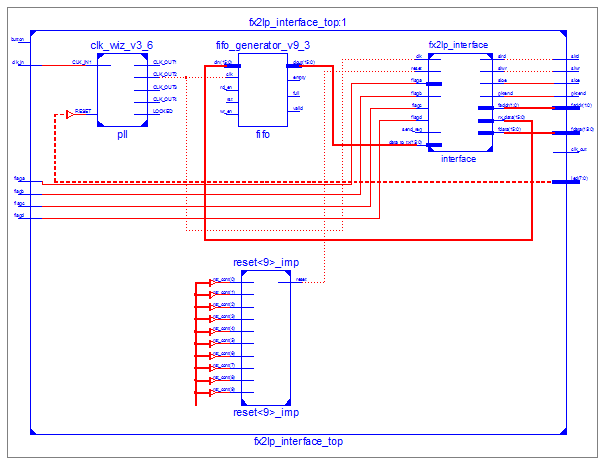
\includegraphics[height=.83\textheight]{fx2lp_rtl}
\end{frame}

\begin{frame}{Verificación Funcional}
	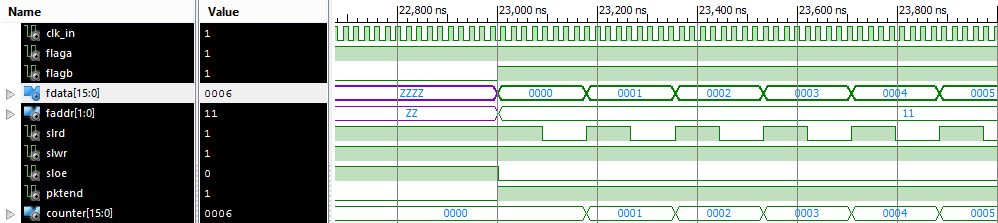
\includegraphics[width=\textwidth]{sist_tb_lect}
\end{frame}

\begin{frame}{Verificación Funcional}
	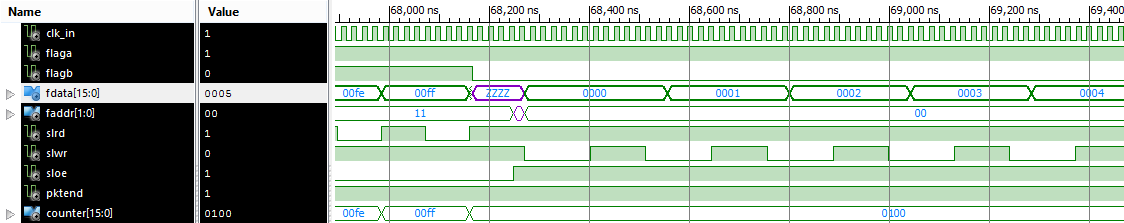
\includegraphics[width=\textwidth]{sist_tb_esc}\\
	\vfill
	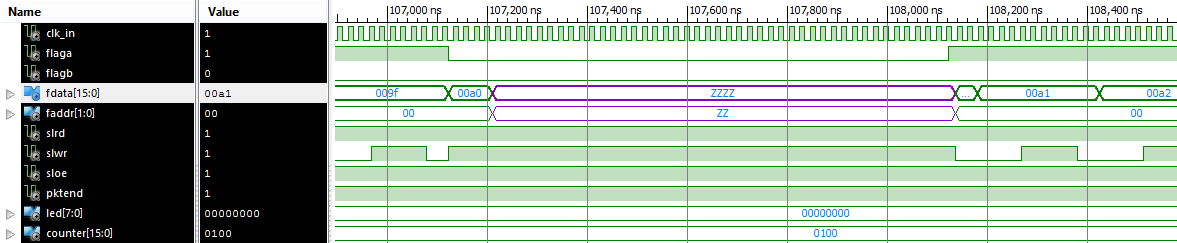
\includegraphics[width=\textwidth]{sist_tb_esc_int}
\end{frame}

\begin{frame}{Verificación Funcional}
	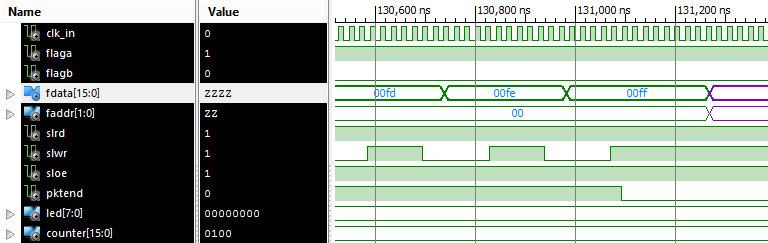
\includegraphics[width=\textwidth]{sist_tb_pktend}
\end{frame}
%\begin{frame}{Test bench - Lectura de la interfaz}
%	\only<1>{
%		\centering
%		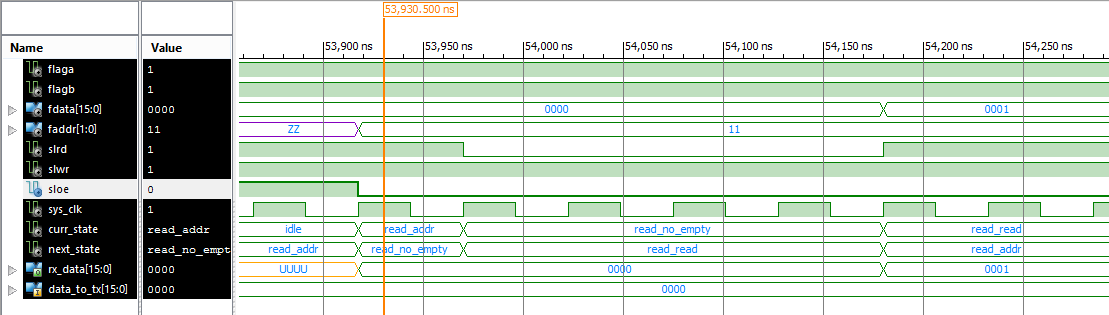
\includegraphics[width=\textwidth]{tb_if_rd_mef}\\
%		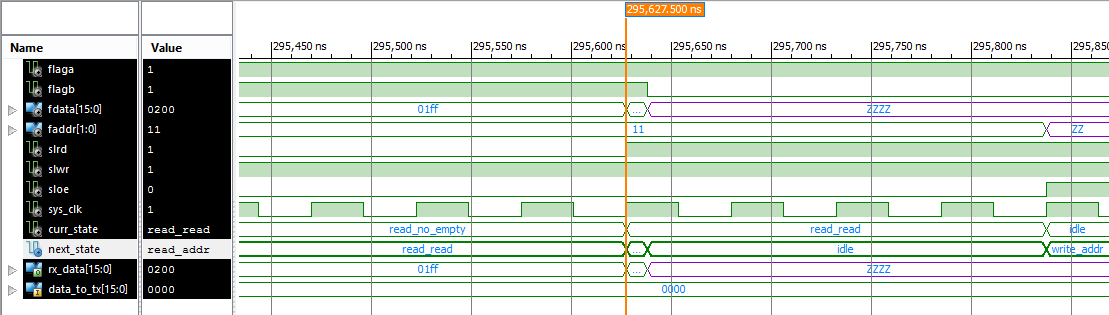
\includegraphics[width=\textwidth]{tb_if_rd_end}
%		}
%\end{frame}
%\begin{frame}{Test bench - Escritura en la interfaz}
%	\only<1>{
%		\centering
%		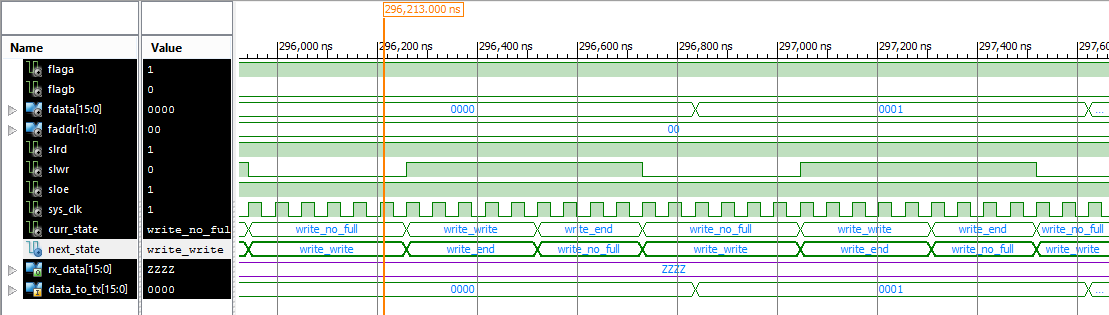
\includegraphics[width=\textwidth]{tb_if_wr_mef}\\
%		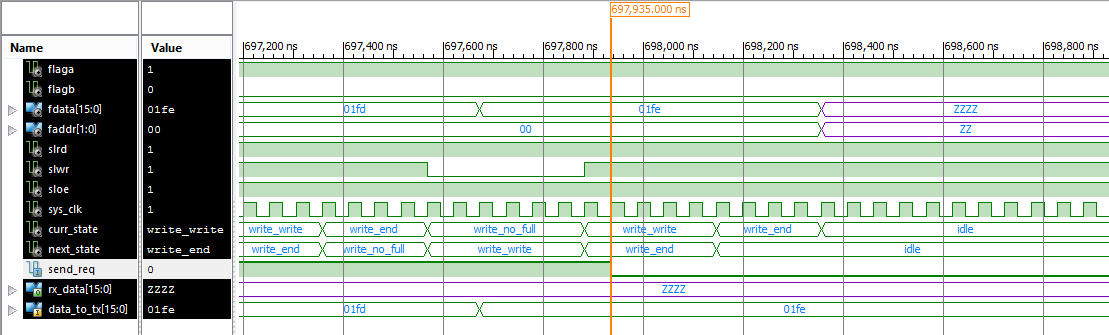
\includegraphics[width=\textwidth]{tb_if_wr_end}}
%	\only<2>{
%		\centering
%		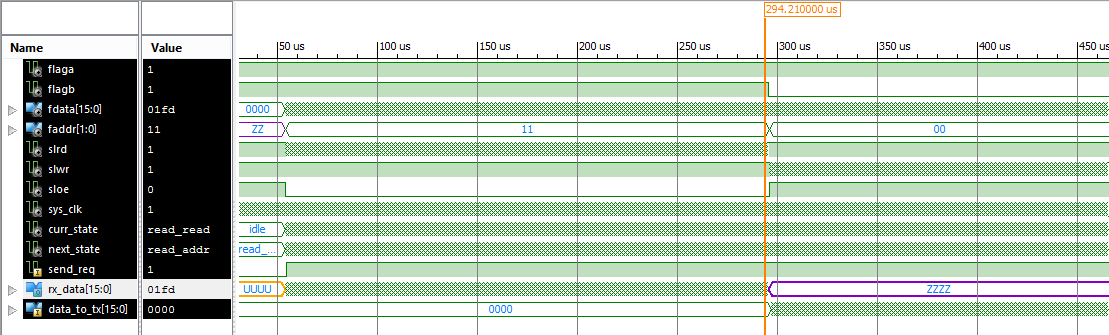
\includegraphics[width=\textwidth]{tb_if_snd}\\
%		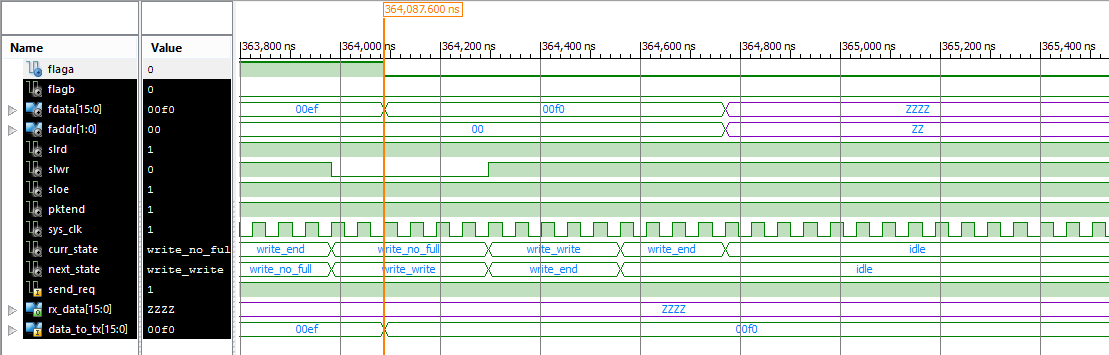
\includegraphics[width=\textwidth]{tb_if_fflag_end}}
%\end{frame}

	\section{Placa de Interconexión}
		\begin{figure}[t]
	\centering
	\begin{subfigure}[t]{0.45\textwidth}
		\centering
		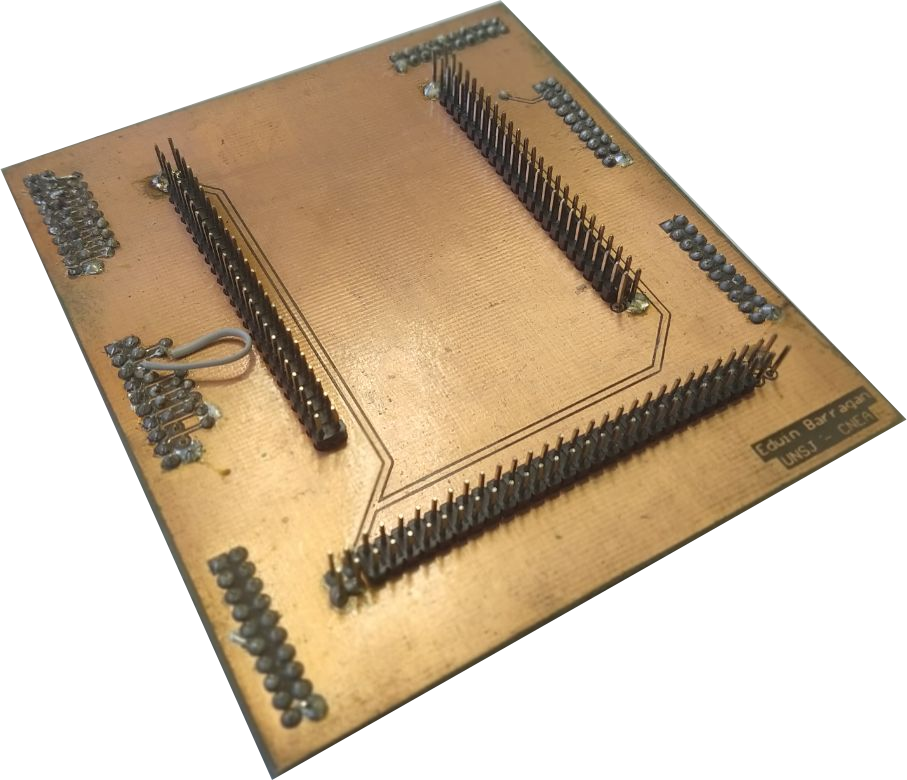
\includegraphics[width=\textwidth]{pcbv2anv}
		\caption*{Anverso}
	\end{subfigure}
	\begin{subfigure}[t]{0.45\textwidth}
		\centering
		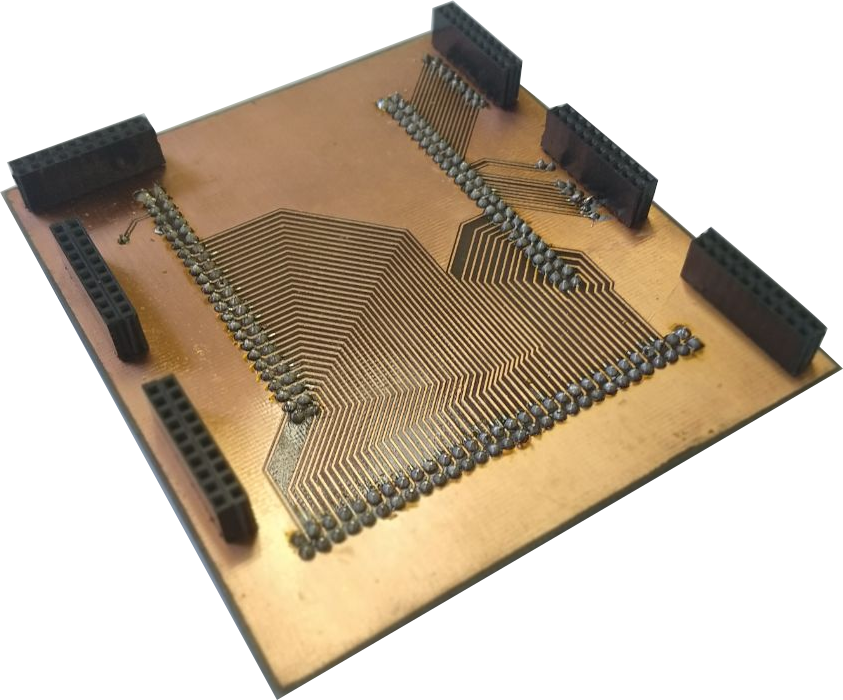
\includegraphics[width=\textwidth]{pcbv2rev}
		\caption*{Reverso}
	\end{subfigure}
	\caption{Versión 2 de la placa de interconexión}
	\label{fpga:pcb:v2}
\end{figure}

Los circuitos integrados utilizados para la implementación de la comunicación USB, estos son el controlador FX2LP de Cypress y el FPGA Spartan VI de Xilinx, vienen incorporados en sendas placas de desarrollo. Para la conexión eléctrica de estos dos chips, se desarrolló una placa de interconexión, es decir, un circuito impreso (PCB, del ingles {\it Printed Circuit Board}) que conecta en forma eléctrica dos o más dispositivos. Esto brinda una conexión mucho más robusta y prolija que si fuese realizada mediante cables cintas o alambres individuales. La Figura \ref{fpga:pcb:v2} muestra el circuito impreso desarrollado. El plano esquemático utilizado para su fabricación se puede consultar en el Anexo \ref{an:pcb}.

%\begin{figure}[ht]
%	\centering
%	\begin{subfigure}[t]{0.45\textwidth}
%		\centering
%		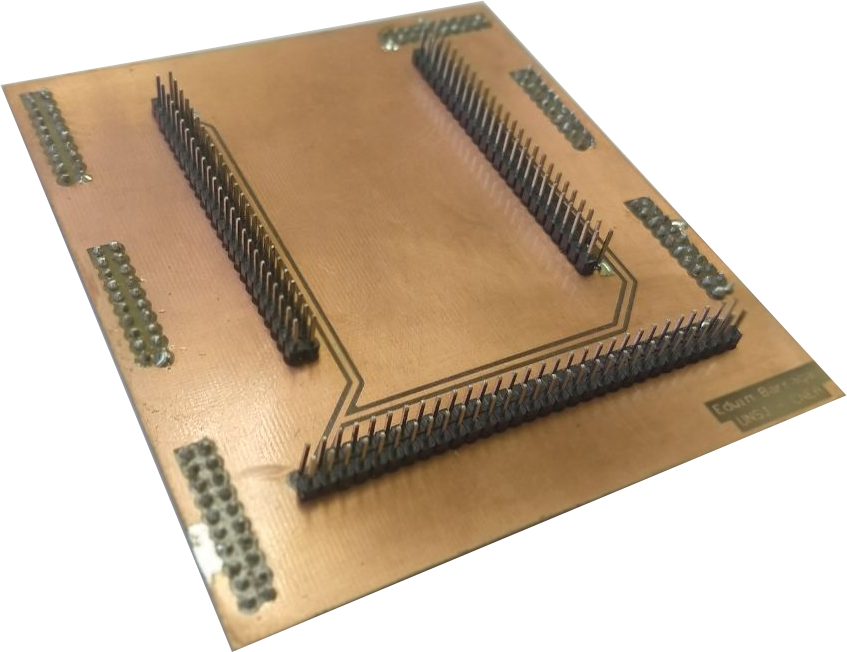
\includegraphics[width=\textwidth]{pcbv1anv}
%		\caption*{Anverso}
%	\end{subfigure}
%	\begin{subfigure}[t]{0.45\textwidth}
%		\centering
%		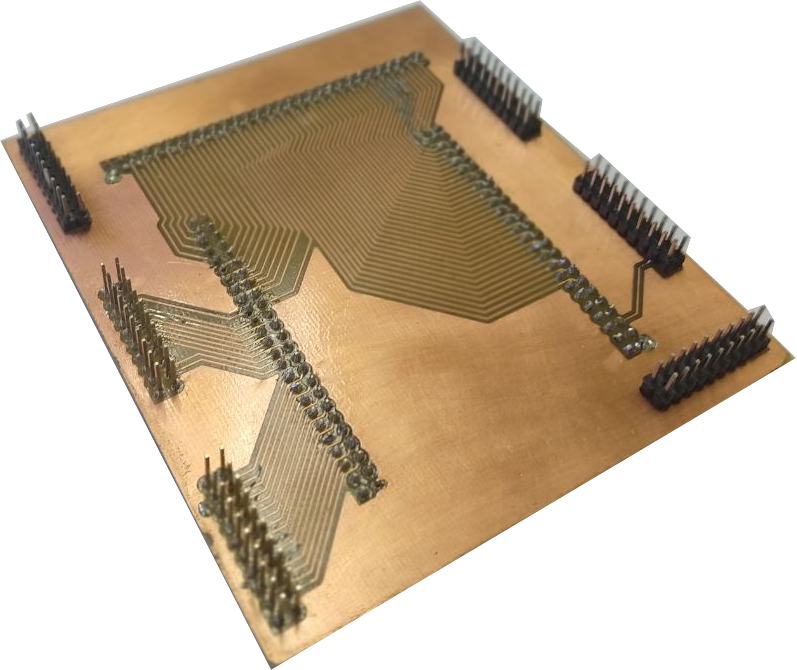
\includegraphics[width=\textwidth]{pcbv1rev}
%		\caption*{Reverso}
%	\end{subfigure}
%	\caption{Versión 1 de la placa de interconexión}
%	\label{fpga:pcb:v1}
%\end{figure}
%
%El desarrollo de la placa de interconexión, necesitó de tres versiones para obtener un correcto funcionamiento. La versión número 1, la cual se observa en la Figura \ref{fpga:pcb:v1}, presenta un problema de contacto eléctrico entre sus dos caras conductoras, debido a no se contaba con la tecnología suficiente para realizar la metalización de los agujeros que conducen la señal de un lado al otro del circuito impreso durante el proceso de fabricación. Por otro lado, en la etapa de montaje, el alumno confunde los pines que debe ser colocados, ya que el reverso necesita pines hembra en lugar de pines macho.
%

%
%Se realiza una segunda versión, la que se observa en la Figura \ref{fpga:pcb:v2}. A este PCB se le incorporan vías pasantes para poder conectar las distintas pistas que recorren el circuito mediante la soldadura de alambres, lo que soluciona el problema de conexión eléctrica. En esta placa se tiene mayor cuidado en la etapa de montaje de los pines. Sin embargo, durante la revisión de los pines se encuentra un defecto en el puerto asignado a la señal de reloj, la cual posee un terminal en un pin que no se encuentra disponible. Esto obliga a la implementación de la comunicación del presente trabajo de forma asíncrona.
%
%Otro defecto que presenta la versión 2 de la placa de interconexión es la inexistencia de un punto para soldadura, que se ocasiona al momento del perforado del impreso. Esto obliga a realizar una conexión mediante un pequeño cable, el cual se puede observar en el anverso de la Figura \ref{fpga:pcb:v2}.
%
%\begin{figure}[ht]
%	\centering
%	\begin{subfigure}[t]{0.45\textwidth}
%		\centering
%		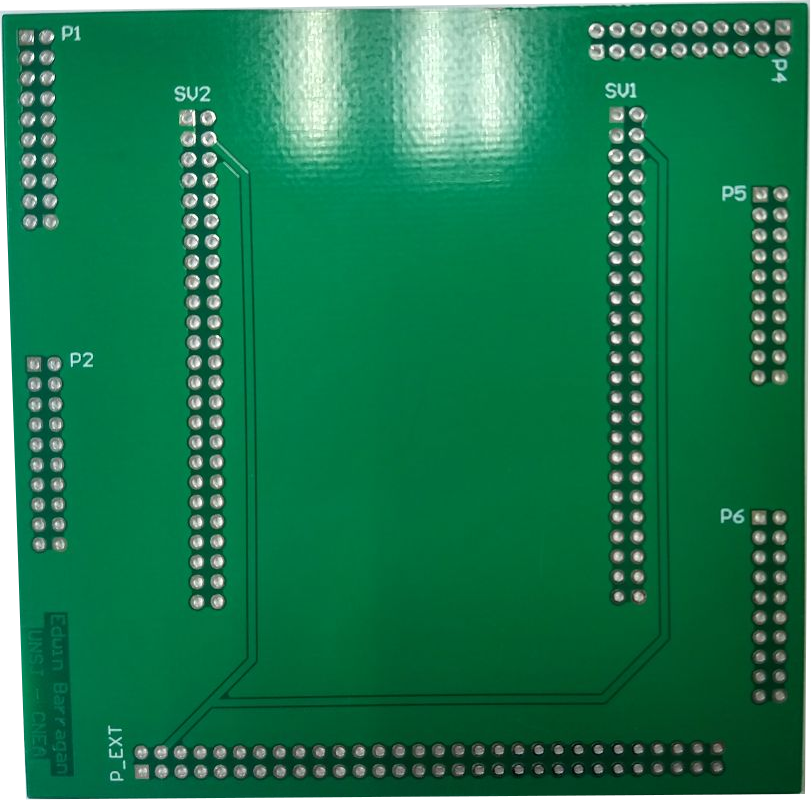
\includegraphics[width=\textwidth]{pcbv3anv}
%		\caption*{Anverso}
%	\end{subfigure}
%	\begin{subfigure}[t]{0.45\textwidth}
%		\centering
%		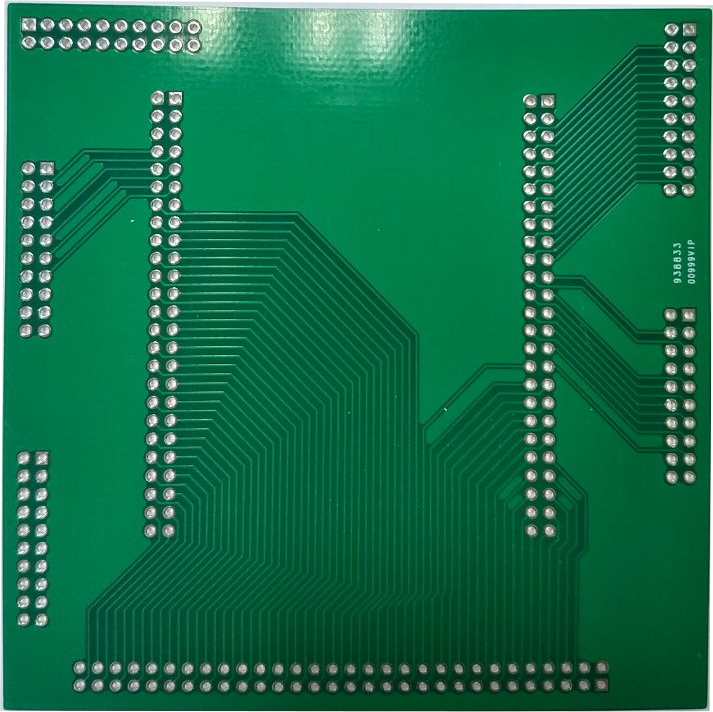
\includegraphics[width=\textwidth]{pcbv3rev}
%		\caption*{Reverso}
%	\end{subfigure}
%	\caption{Versión 3 de la placa de interconexión}
%	\label{fpga:pcb:v3}
%\end{figure}
%
%Finalmente, se decide rehacer el circuito de conexión en una tercera versión y solicitar su fabricación en una empresa especializada en la manufactura de PCB para prototipo, radicada en China. En esta versión, fue redirigida la línea de conexión defectuosa, lo que permite conectar las fuentes de reloj e implementar una comunicación síncrónica. Esto no fue realizado al momento de la escritura del presente informe, aunque se espera su implementación en trabajos futuros. Además, debido a restricciones en el proceso de fabricación, se debe redimensionar el PCB y hacerlo más compacto.
%
%Gracias a la mejora que brinda la empresa en el proceso de fabricación, se eliminan las conexiones entre las dos caras del impreso mediante la soldadura de alambre y se cambian por agujeros metalizados. Además, se incorporaron conexiones adicionales entre el controlador y el FPGA. Esto permite utilizar el $\mu$C 8051 incorporado al controlador FX2LP para realizar tareas adicionales, junto al FPGA. Se adjunta en el Anexo \ref{an:pcb} un plano esquemático con las conexiones de la versión 3 del circuito impreso. elaborado.
	\section{Sumario del capítulo}
		En el presente capítulo se desarrolló y justificó la elección del controlador FX2LP como nexo entre la FPGA y la PC, brindando la conexión USB necesaria. Luego, se explicaron algunos componentes de la arquitectura implementada por Cypress a fin de proveer la comunicación USB. Finalmente, se detalló paso a paso cada uno de los componentes configurados, como así también el código desarrollado para dicho fin.

Además, se mostraron algunos detalles del framework provisto por Cypress y los encabezados necesarios para su utilización y se explicitaron los descriptores a través de los cuales se le informa al sistema las características de la comunicación que se implementa.
%	\chapter{Verificación y validación del sistema}
	\label{cap:verif}
	La interfaz que este trabajo utiliza para que los datos fluyan entre un FPGA y una PC está compuesta por el controlador EZ-USB FX2LP de Cypress, el cual viene incorporado en el kit de desarrollo CY3684.

El kit de desarrollo CY3684 puede ser descompuesto en dos partes: una de hardware, que posibilita la conexión eléctrica entre los componentes y una parte de software que facilita al desarrollador tanto la elaboración del programa que es cargado en y ejecutado por el microcontrolador, denominado firmware, como las pruebas del sistema en desarrollo.

Este Capítulo aborda algunos aspectos conceptuales sobre la estructura y arquitectura del circuito integrado EZ-USB FX2LP y desarrolla
la configuración seleccionada, la elaboración del firmware y las herramientas utilizadas.%Un puerto USB posee una estructura fija: 4 contactos; dos de alimentación y dos datos. A su vez, el Protocolo USB es muy específico en cuanto a los niveles de tensión, la frecuencia de comunicación, las cadenas de bits clave que deben enviarse, entre muchas otras cosas que detalla la {Norma USB 2.0}\cite{Compaq2000}.%\\

%Un FPGA, en contraste con lo anterior, es un dispositivo electrónico que posee en su interior una gran cantidad de elemento lógicos programables. Esto permite la síntesis de casi cualquier circuito lógico. Dicha síntesis puede poseer la cantidad y disposicion de puertos como pines posea el FPGA, exceptuando algunas entradas específicas para el funcionamiento del FPGA. Esto configura una gran versatilidad que permite ajustar un sistema desarrollado dentro del FPGA a la medida necesaria.%\\

%El nexo entre los datos que se producen en sistema en el que se desenvuelve un FPGA y un puerto USB, se lo denomina interfaz. Esta última, en el presente trabajo, está compuesta por un circuito integrado particular, cuya codificación comercial es CY7C68013A, fabricado por Cypress Semiconductor. Este componente electrónico pertenece a la familia de controladores FX2LP del catálogo de integrados EZ-USB. El chip CY7C68013A se encuentra incorporado el kit de desarrollo CY3684 EZ-USB Development Kit, provisto por el fabricante.%\\

%Un kit de desarrollo es un conjunto de herramientas que permiten elaborar soluciones electrónicas que requieren un componente en particular. Además, cuenta con algunos dispositivos genéricos que posibilitan emular el sistema que utilizará el componente central del kit. En el caso del kit que se utiliza en este trabajo se descompone en dos grandes grupos: hardware y software. En la parte de hardware se incluye de un circuito impreso (PCB) que posee soldado, el integrado que nos servira de interfaz y otros componentes que se describen en el Capítulo \ref{cap:mats}.%\\

%En lo que a software se refiere, Cypress incorpora en el kit de desarrollo un código marco que posee escritas todas las funciones y registros que ejecutan las tareas que el sistema necesita para llevar a cabo la comunicación USB. Además se cuenta con herramientas de software que permite escribri, compilar y cargar el programa que se ejecuta en el controlador FX2LP.%\\

%En este capítulo se desarrolla la arquitectura de los integrados FX2LP y se abordan los módulos más relevantes para este trabajo. También se explican las herramientas del kit que fueron utilizadas para la elaboración del firmware y, finalmente, los aspectos más sobresalientes del firmware que ejecuta el CY7C68013A, y establece el funcionamiento de la comunicación USB.
	\section{Depuración de la configuración de la interfaz FX2LP}
		%Durante el desarrollo de este trabajo, se halló un problema importante sobre la compilación y ejecución del código escrito en C para microcontroladores. Dicho problema consiste en 

%Durante el desarrollo del código precedentemente explicado, 
Se realizaron diversas pruebas y versiones tanto para resolver problemas como para verificar el correcto funcionamiento de la interfaz.

El primer problema que se presentó fue una inestabilidad en la ejecución del código, la cual se mostraba en forma intermitente al cargar el código compilado. La inestabilidad hacía que el código repentinamente se detuviera en la ejecución de la inicialización del dispositivo. A fin de salvar dicho problema, se recurrió al envío de mensajes de seguimiento a través de los puertos UART que prevee el controlador FX2LP.

También se realizaron pruebas de robustez en la comunicación, pudiendo enviar y recibir datos por el mismo puerto UART, aprovechando la configuración establecida. Para la recepcion de datos en la PC se utilizó el programa Hercules\cite{HWGroup}. Dicho programa es una desarrollo cuya descarga es libre y permite configurar y recibir mensajes a través de diferentes puertos.

Como testigo del funcionamiento de los flags, se asociaron sus valores a los LED de propósito general, de forma tal que se pueda corroborar que los endpoint usados recibian y enviaban los datos cuando se emitía la orden desde el Host.

\subsection{Biblioteca FX2LPSerial}
Para la configuración y utilización del puerto UART 0 se recurrió a la biblioteca FX2LPSerial\cite{Kumar2017}. Esta biblioteca es un conjunto de funciones de C para microcontroladores que resuelven la configuración los puertos UART y de las rutinas asociada a la recepción y envío de datos por dichos puertos. 

La configuración del puerto UART se realizó a través de la función \verb|FX2LPSerial_Init()|. Esta función configura los registros de los contadores para establecer una tasa de transmión de 38400 baudios. Luego, asegura que el reloj que utiliza el puerto UART se encuentre configurado. Esto se realiza a través del Registro de Configuración de la Interfaz (IFCONFIG), el cual se setea para correr a \SI{48}{\mega\hertz}, la misma a la cual funciona el sistema desarrollado, por lo que no presenta problemas de compatibilidad. Si bien es posible cambiar la velocidad de transmisión, esta configuración posee una desviación del 0,16\%\cite{CypressSemiconductor2014fx2lp} entre la tasa nominal y la tasa real de transferencia. Esta diferencia de tasas es suficiente para asegurar que funcione en cualquier dispositivo. Por lo tanto, se decidió utilizar la configuración con los valores por defecto.

%Durante la compilación y ejecución de las tareas provista por Cyress a traves de su framework, sucedió que de forma inesperada, el controldaor FX2LP no lograra inicializar en forma correcta su funcionamiento. Se dice que sucedía en forma inesperada ya que no había causa aparente para este comportamiento anómalo: el compilador no informaba error alguno y el código desarrollado no tenía nada de malo luego de diversa revisiones.

%Para verificar el código desarrollado, se utilizó un programa monitor precompilado, el cual es provisto por Cypress. Este monitor permite al desarrollador acceder a operaciones de depuración, tales como el chequeo de variables, el pausado y reanudado de ejecuciones, etc. El desarrollo realizado funcionó sin inconvenientes a través de este monitor.

%Luego, se buscó correr el programa con alguna función que permitiese seguir la ejecución de la rutina implementada. Para ello, se utilizó la biblioteca FX2LPSerial\cite{Kumar2017}. Esta biblioteca es un conjunto de funciones de C para microcontroladores que se sirven para configurar los puertos UART y de las rutinas asociada a la recepción y envío de datos por dichos puertos. Así, se configuró el envió de mensajes por UART y que luego se recibieron en una PC.

%La configuración del puerto UART se realizó a través de la función \verb|FX2LPSerial_Init()|. Esta función configura los registros de los contadores para establecer una tasa de transmión de 38400 baudios. Luego, asegura que el reloj que utiliza el puerto UART se encuentre configurado. Esto se realiza a través del Registro de Configuración de la Interfaz (IFCONFIG), el cual se setea para correr a \SI{48}{\mega\hertz}, la misma a la cual funciona el sistema desarrollado, por lo que no presenta problemas de compatibilidad.Si bien es posible cambiar la velocidad de transmisión, esta configuración posee un diferencia del 0,16\%\cite{CypressSemiconductor2014fx2lp}, lo que asegura que funcione en cualquier dispositivo, por lo tanto, se decidió dejarla tal cual está.

Para la recepcion de datos en la PC se utilizó el programa Hercules\cite{HWGroup}. Dicho programa es de descarga libre y permite configurar y recibir mensajes a través de protocolo Ethernet o por puerto Serie. Se configuró el puerto UART, en la pestaña destinada al monitoreo del puerto Serie, con una tasa de transmisión de 38400 baudios, 8 bit, sin paridad y sin handshaking. A través de esta configuración recibie cualquier dato enviado a través de los puertos UART del controlador FX2PL y los muestra en formato ASCII.

Una vez configurado el envío de datos a través del puerto UART, se procedió a enviar mensajes de control para poder corroborar la funcionalidad y comprobar si efectivamente el controlador efectuaba sus tareas y en que momento dejaba de hacerlo.

Se pudo determinar que en la función \verb|main()|, luego de realizar la inicialización de todos los modulos, procede a la desconexión del controlador con el puerto USB, a través de una rutina que Cypress denomina ReNumertion\cite{CypressSemiconductor2014fx2lp}. Durante la reconexión ocurre algún efecto, aún no identificado, que hace que el programa se detenga cuando debe reconectarse. Este desperfecto fue solucionado con el agregado de una línea de comunicación después de el activado del reconcetado. Esto demostró ser lo suficientemente robusto ya que eliminando todas las  líneas que envían datos de monitoreo no aparació nuevamente la detención del programa, más sí, eliminando solo esa línea de código. De esta manera, el código queda de la siguiente forma en donde la línea 190 es la agregada en este trabajo:

\begin{lstlisting}[language=C,backgroundcolor=\color{gray!30},numbers=left,firstnumber=189,basicstyle=\footnotesize]
	 USBCS &=~bmDISCON;
	 FX2LPSerial_XmitString("Reconectando...\n\n");
\end{lstlisting}

\subsection{Testigos LED}
Los LED multipropósito incorporados en la placa de desarrollo CY3684, fueron programados para que repliquen el estado de los flags de vaciado y de llenado de los EP. De esta forma, se pudo monitorear la carga de datos en el controlador y la descarga a través del puerto USB y vicersa.

Los LED se encuentran conectados a través de un decodificador. Para su encendido, es necesario la lectura de las direcciones hexadecimales de memoria 80xx, 90xx, A0xx y B0xx, mientras que para su apagado, las direcciones a leer son  88xx, 98xx, A8xx y B8xx\cite{CypressSemiconductor2014cy3648}. Por ello, se elaboró el encabezado {\it leds.h}, el que se observa a continuación.
	
	\begin{lstlisting}[language=C,backgroundcolor=\color{gray!30}]
	xdata volatile const BYTE D2ON	_at_ 0x8800;
	xdata volatile const BYTE D2OFF	_at_ 0x8000;
	xdata volatile const BYTE D3ON	_at_ 0x9800;
	xdata volatile const BYTE D3OFF	_at_ 0x9000;
	xdata volatile const BYTE D4ON	_at_ 0xA800;
	xdata volatile const BYTE D4OFF	_at_ 0xA000;
	xdata volatile const BYTE D5ON	_at_ 0xB800;
	xdata volatile const BYTE D5OFF	_at_ 0xB000;	\end{lstlisting}
	
Luego, con el propósito de enceder o apagar los diodos emisores de luz, es necesario declarar una variable auxiliar y asignarle los punteros declarados. Así, a través de la función \verb|TD_Poll()|, que es la función que se ejecuta en el loop infinito del controlodaro FX2LP, se colocó la el siguiente código:

	\begin{lstlisting}[language=C,backgroundcolor=\color{gray!30}]
void TD_Poll(void)             // Called repeatedly while the device is idle  
{
	BYTE dum;
	
	if(EP8FIFOFLGS & bmBIT1)//ep8 fifo empty
	{
		dum = D4ON;
	}
	else
	{
		dum = D4OFF;
	}

	if(EP8FIFOFLGS & bmBIT0)//ep8 fifo full
	{
		dum = D3ON;
	}
	else
	{
		dum = D3OFF;
	}
	if(EP2FIFOFLGS & bmBIT1)//ep2 fifo empty
	{
		dum = D2ON;
	}
	else
	{
		dum = D2OFF;
	}
}
	\end{lstlisting}

A través de los registros EPxFIFOFLGS se puede conocer el estado de cada uno. Aplicando una máscara bit a bit, se obtiene el estado de cada uno de los flags. Así, dependiendo del estado de cada uno de ellos, se enciende o se apagan las luces.
Esta rutina resultó de mucha utilidad a la hora de realizar las diferentes pruebas, tanto del funcionamiento de la interfaz, como de la conexión entre la itnterfaz y el FPGA.

\subsection{Prueba de envío y recepcion de datos}
	Para la verificación de la conexión entre la PC y la interfaz, a través del protocolo USB, se utilizó el programa {\it Cypress USB Control Center}, provisto por Cypress dentro del kit de desarrollo CY3684, con el cual se desarrolló este trabajo. Dicho software permite cagar el firmware desarrollado en la interfaz y, a su vez, detalla la información recibida a través de los descriptores y posibilita el envío y recepción de mensajes.
	
	Para corroborar que el envío de datos fue existoso, se procedió a enviar datos a través del {\it Cypress USB Control Center}. Así, en primer lugar, corroborando que el LED que indica que el EP8 se encuentra vacío se apaga, se infirió que los datos estaban llegando. A continuación, se enviaron más datos hasta lograr que el LED asociado al límite de capacidad del EP8 se encendiese. Luego, a través de un pulsador, se activa una rutina de envío de los datos guardados en el EP8 a través del puerto UART. Para ello, fue necesario realizar unos pequeños ajustes en la configuración.
	
	El controlador FX2LP de Cypress permite manipular los datos de los paquetes USB. Sin embargo, la configuración por defecto, no permite realizar esta tarea. Para ello es necesario, en primer lugar, desactivar lo que Cypress llama el armado automático de paquetes y habilitar la manipulación avanzada de paquetes\cite{CypressSemiconductor2014fx2lp}.
	
	A medida que los datos van ingresando al controlador FX2LP a través del puerto USB, el Motor de Interfaz Serial (MIS) los coloca en el espacio de memoria asignado y va incrementando un contador por cada byte recibido. De esta forma, la interfaz puede saber cuantos datos, efectivamente, posee almacenados. Sin embargo, cuando los datos ingresan a través de la memoria FIFO, es otro el contador incrementado. El armado automático de paquetes realiza la tarea de emparejar estos contadores, de forma tal que no se deba destinar tiempo de ejecución de $\mu$C para esta tarea.
	
	Para poder escribir datos en la memoria y informarle al MIS que se agregaron datos, es necesario que este armado autmático está desactivado. Esto implica que cuando lleguen datos, el controlador debe poder realizar esta operación. A su vez, por defecto los paquetes que llegan desde la PC no pueden ser modificados. Para realizar esto, es necesario hablitar el manejo mejorado de paquetes. Tanto la manipulación avanzada de paquetes como el armado automático se encuentran los dos bits menos significativos del Registro de Control de Revisión (REVCTL).
	
	Una vez activados ambos bits del registro REVCTL, se debe efectuar la rutina que armará los paquetes en forma ``manual''. Para este propósito, se activó una interrupción que se dispara cada vez que llegan mensajes a un EP determinado, en este caso, el EP8. Toda esta configuración se realizó en las últimas líneas de la función \verb|TV_Init()|, la cual quedó de la siguiente forma:
	
	\begin{lstlisting}[language=C,backgroundcolor={gray!30}]
	
	\end{lstlisting}
	%Uso de Interrupciones
	%Uso de pulsasdores
	%Sobre RevCtl 
	\section{Pruebas de la síntesis de la MEA en el FPGA}
		%INTENTO 1

%En el Capítulo \ref{cap:int} se detalló que el sisetma desarrollado se compone de tres componentes principales, a saber: El Host, cuyo rol es llevado a cabo por una PC; la interfaz, integrada por el controlador FX2LP de Cypress y un FPGA, en este caso un Spartan-6 de Xilinx. A su vez, el Capítulo \ref{cap:fpga}, indica que el sistema interno del FPGA lleva una Maquina de Estados Finitos (MEF), cuya función es la de realizar el efectivo intercambio de datos con la interfaz, y un sistema genérico.
%
%Hasta acá se ha desarrollado la configuración de la interfaz y la implementación de la MEF. Sin embargo, es necesario, que el sistema pueda funcionar en forma autónoma, proveerle un sistema mínimo que pueda hacer las veces de fuente y sumidero de datos. Es por esto, que se dotó al sistema con una memoria FIFO con el objetivo de implementar un eco que permita realizar una evaluación de desempeño de la comunicación desarrollada. Así, se permite enviar mensajes desde una PC y que estos sean recibidos luego.
%
%\subsection{Implementación de la memoria FIFO en el FPGA}
%	La memoria FIFO sintetizada en el FPGA se obtuvo a través de la herramienta {\it Core Generator} provista por Xilinx junto con el entorno de desarrollo ISE, utilizado en este trabajo para el desarrollo\cite{XilinxInc}. La configruación seleccionada generó una memoria FIFO de 511 bytes, con puertos de entrada y salida dedicados, es decir uno de entrada y uno de salida, un bus de 16 bits de ancho. Posee señal de reconocimiento de escritura. También se dotó a la memoria generada con entradas de reloj y habilitación de bus independientes tanto para el puerto de entrada como el puerto de salida.
%	
%	
%INTENTO 2
%TODO debería decir como generar cada una de las señales internas propuesas en el capitulo correspondiente... la magen en cuestion es \ref{fpga:intersignal}
Con el objetivo de verificar el sistema desarrollado, se procedió a implementarlo en un sistema mínimo que sea capaz de utilizar la comunicación, de forma tal que el Host pueda establecer un enlace con el FPGA. Para ello, se implementó un sistema eco, es decir, un sistema que recibe los mensajes que envía el Host y, luego, los transmite para que el Host pueda recibirlos. De esta forma, el Host puede reconocer que los datos enviados no fueron perdidos ni modificados.

\begin{figure}[ht]
	\centering
	\begin{tikzpicture}[scale=.7]
		\begin{scope}[transform shape,node distance=4,>=latex,double distance=1.3]
			\node[simple](fx2lp){Interfaz FX2LP};
			
			\node[simple, rounded corners,minimum size=80] (PC)[left=2 of fx2lp]{PC};
			\draw[double,<->](PC) -- node[above]{USB} (fx2lp);
			
			\node[simple](mea)[right=of fx2lp]{Maquina de Estados Algorítmica};
			
			\draw[double,<->] ([yshift=3.5*110/4]fx2lp.east)-- node [above]{FDATA[15:0]} ([yshift=3.5*110/4]mea.west);
			\draw[double,<->] ([yshift=2.5*110/4]fx2lp.east)-- node [above]{FADDR[1:0]} ([yshift=2.5*110/4]mea.west);
			\draw[->] ([yshift=1.5*110/4]fx2lp.east)--node[above]{FLAG\_Vacío} ([yshift=1.5*110/4]mea.west);
			\draw[->]([yshift=.5*110/4]fx2lp.east)--node[above]{FLAG\_Lleno}([yshift=.5*110/4]mea.west);
			\draw[<-]([yshift=-.5*110/4]fx2lp.east)--node[above]{SLOE}([yshift=-.5*110/4]mea.west);
			\draw[<-]([yshift=-1.5*110/4]fx2lp.east)--node[above]{SLRD}([yshift=-1.5*110/4]mea.west);
			\draw[<-]([yshift=-2.5*110/4]fx2lp.east)--node[above]{SLWR}([yshift=-2.5*110/4]mea.west);
			\draw[<-]([yshift=-3.5*110/4]fx2lp.east)--node[above]{PKTEND}([yshift=-3.5*110/4]mea.west);
			
			\node[simple,minimum size=50](clk)[right=of mea.south east,anchor=south west] {PLL};
			\draw[<-]([]mea.east |- clk.west)--node[above]{Reloj}([]clk.west);
%			\draw[<-]([yshift=-1*80/3]mea.north east)--node[above]{Reloj}([yshift=-1*80/3]clk.north west);
%			\draw[<-]([yshift=-2*80/3]mea.north east)--node[above]{Reset}([yshift=-2*80/3]clk.north west);
			\node[rounded corners,simple, minimum size=50](clkSrc)[below=1 of clk]{Fuente de reloj};
			\draw[->](clkSrc) to (clk);
			
			\node[simple,minimum height=150,minimum width=50](interno)[right=of mea.north east,anchor=north west]{Memoria FIFO};
			\draw[double,->]([yshift=-.5*150/6]mea.north east)--node[above]{Dato\_enviado[15:0]} ([yshift=-.5*150/6]interno.north west);
			\draw[double,<-]([yshift=-1.5*150/6]mea.north east)--node[above]{Dato\_a\_enviar[15:0]}([yshift=-1.5*150/6]interno.north west);
			\draw[<-]([yshift=-2.5*150/6]mea.north east)--node[above]{Enviar\_datos}([yshift=-2.5*150/6]interno.north west);
			\draw[->]([yshift=-3.5*150/6]mea.north east)--node[above]{SLRD}([yshift=-3.5*150/6]interno.north west);
			\draw[->]([yshift=-4.5*150/6]mea.north east)--node[above]{SLWR}([yshift=-4.5*150/6]interno.north west);
			\draw[<-]([yshift=-5.5*150/6]mea.north east)--node[above]{PKTEND}([yshift=-5.5*150/6]interno.north west);
			
		\end{scope}
		\begin{scope}[]
			\node[rounded corners,inner ysep=5pt,draw=black,rectangle,fit={(mea)(interno)},label=north:FPGA](fpga){};
			\node[inner ysep=11pt, yshift= 8pt, draw=black,rectangle,fit={(fpga)(clkSrc)},label=north:Mojo](){};
		\end{scope}
	\end{tikzpicture}
	\caption{Diagrama en bloques del sistema de prueba}
	\label{test:sist}
\end{figure}

Para establecer un sistema eco, se deben implementar todas las señales de control que se observan en la Figura \ref{fpga:intersignal}. Estas son, señal de reset, señal de reloj, solicitud  sde envío de datos y los datos a enviar. A su vez, se deben poder leer los datos recibidos y las señales {\it SLWR} y {\it SLRD}, a través de las cuales el sistema señala el cambio de dato. 

Con el objetivo de poder recibir, almacear y reenviar los datos que llegan desde la interfaz, se sintetizó en el FPGA una memoria FIFO que almacene los datos y, cuando el EP de salida no posee más datos, es decir que el {\it Flag Vacío} se encuentra activo, retransmita los datos hacia la interfaz hasta que el Host los solicite.

Una vez incorporados los componentes al FPGA, se realizó su validación funcional antes de ser cargado todo el desarrollo al FPGA para efectuar las pruebas del sistema. A continuación, se detallarán los componentes y señales que se sintetizaron, como así también la verificación realizada.

\subsection{Declaración de la entidad}
	Para la implementación y síntesis del sistema, es necesario declarar los puertos que tendrán una correspondencia física con un pin de salida del FPGA en la descripción de mayor jerarquía. El archivo que posee una mayor jerarquía es usualmente llamada top.
	
	Como se conoce cuáles son las señales a través de las cuales el FPGA debe conectarse con la interfaz, es posible declarar la entidad que se sintetizó. Además se declararó  la señal de reloj, que proviene desde la placa Mojo v3. El código de descripción en donde se declaró la entidad se muestra a continuación.
	
	\begin{lstlisting}[language=VHDL,backgroundcolor=\color{gray!30}]
entity fx2lp_interface_top is
	generic(
		constant in_ep_addr:	std_logic_vector(1 downto 0) := "00";
		constant out_ep_addr:	std_logic_vector(1 downto 0) := "11";
		constant port_width: integer := 16
		);
	port(
		fdata   : inout std_logic_vector(port_width-1 downto 0);  
		faddr   : out   std_logic_vector(1 downto 0);
		slrd    : out   std_logic;
		slwr    : out   std_logic;
		flaga   : in    std_logic;
		flagb   : in    std_logic;
		flagc   : in    std_logic;
		flagd   : in    std_logic;
		sloe    : out   std_logic;
		pktend  : out   std_logic;
		clk_in  : in    std_logic
		);
end fx2lp_interface_top;
	\end{lstlisting}

\subsection{Instanciación de la MEF}
		Dentro de los componentes incorporado al sistema, el más importante es la MEF elaborada en el Capitulo \ref{cap:fpga}, debido a que es el componente que se desea sintetizar, verificar y probar. Para que el sistema reconozca que ese módulo debe incorporarlo al sistema, se declaró como componente los puertos de la entidad elaborada en el capítulo mencionado y se lo instanció como se observa a continuación.
		
		\begin{lstlisting}[language=VHDL,backgroundcolor=\color{gray!30}]
 architecture fx2lp_interface_arq of fx2lp_interface_top is
 	COMPONENT fx2lp_interface
	GENERIC(
		constant in_ep_addr:	std_logic_vector(1 downto 0) := "00";
		constant out_ep_addr:std_logic_vector(1 downto 0) := "11";
		constant port_width: integer := 16
	);
	PORT(
		clk : IN std_logic;
		reset : IN std_logic;
		flaga : IN std_logic;
		flagb : IN std_logic;
		flagc : IN std_logic;
		flagd : IN std_logic;
		send_req : IN std_logic;
		data_to_tx : IN std_logic_vector(15 downto 0);    
		fdata : INOUT std_logic_vector(15 downto 0);      
		faddr : OUT std_logic_vector(1 downto 0);
		slrd : OUT std_logic;
		slwr : OUT std_logic;
		sloe : OUT std_logic;
		pktend : OUT std_logic;
		rx_data : OUT std_logic_vector(15 downto 0)
		);
	END COMPONENT;
 begin
 	interface: fx2lp_interface PORT MAP(
		clk => sys_clk,
		reset => reset,
		fdata => fdata,
		faddr => faddr,
		slrd => slrd_sig,
		slwr => slwr_sig,
		flaga => flaga,
		flagb => flagb,
		flagc => flagc,
		flagd => flagd,
		sloe => sloe,
		pktend => pktend,
		send_req => write_req,
		rx_data => din,
		data_to_tx => dout
	);
[...]
end fx2lp_interface_arq;
		\end{lstlisting}
		
		Se puede observar que las constantes genéricas fueron definidas en la declaración del componente . Sin embargo, estas no fueron instanciadas debido a que la configuración a probar era la asignada por defecto.
		
\subsection{Otros componenetes y señales de control }

	\subsubsection{Generación de Señal de Reloj}
		Las especificaciones de la interfaz indican que la máxima frecuencia de funcionamiento del reloj debe ser de \SI{48}{\mega\hertz}\cite{Cypress2017}. La placa de desarrollo Mojo V3, por su parte, posee un oscilador que provee al FPGA una señal de \SI{50}{\mega\hertz}. Para lograr la señal de reloj con la frecuencia adecuada, se utiliza un PLL incorporado dentro del integrado del FPGA. 
		
		El PLL fue configurado a través de la herrmienta {\it Core Generator} provista por Xilinx junto con el entorno de desarrollo ISE, utilizado en este trabajo para el desarrollo\cite{XilinxInc}. A través de esta herramienta, se indicó que la señal de entrada es de \SI{50}{\mega\hertz}. Luego, con el objetivo de poseer señales de frecuencias diferentes por si se presentaran problemas de sincronismo, se seleccionaron señales de salida de \si{50}, \si{48}, \si{40} y \SI{35}{\mega\hertz}.
		
		La herramienta {\it Core Generator} de Xilinx entregó un código de VHDL en donde se declara una entidad para que pueda ser utilizada como componente y se instancia el PLL. Luego, la entidad de dicho código se declaró e instanció en la descripción del sistema de pruebas de la siguiente forma:
		
		\begin{lstlisting}[language=VHDL,backgroundcolor=\color{gray!30}]
architecture fx2lp_interface_arq of fx2lp_interface_top is
[...]
	component clk_wiz_v3_6
	port(
		CLK_IN1 : in  std_logic;
		CLK_OUT1: out std_logic;
		CLK_OUT2: out std_logic;
		CLK_OUT3: out std_logic;
		CLK_OUT4: out std_logic;
		RESET   : in  std_logic;
		LOCKED  : out std_logic
	);
	end component;
[...]
begin
	pll : clk_wiz_v3_6 
		port map(
			CLK_IN1   => clk_in,
			CLK_OUT1  => pll_50,
			CLK_OUT2  => pll_48,
			CLK_OUT3  => pll_40,
			CLK_OUT4  => pll_35,
			RESET     => '0',
			LOCKED    => locked
		);
	
		sys_clk <= pll_48;
[...]
end fx2lp_interface_arq;
		\end{lstlisting}
		
		Se puede notar que las señales {\it pll\_50}, {\it pll\_48}, {\it pll\_40} y {\it pll\_35} se utilizaron de manera especial para seleccionar en forma rápida la frecuencia que se le asigna a la señal de reloj del sistema. La señal asgnada al reloj del sistema fue la salida del PLL que posee una frecuencia de \SI{48}{\mega\hertz}.
		
	\subsubsection{Generación de señal de reset}
		La señal de reset fue generada por un contador con el objetivo de asegurar que, al conectar el FPGA, el sistema espere que finalice cualquier transitorio que pueda causar respuestas inesperadas e inicie con los valores iniciales preestablecidos.

		\begin{lstlisting}[language=VHDL,backgroundcolor=\color{gray!30}]
	init_rst: process(sys_clk)
	begin
		if rst_cont /= 0 then
			if rising_edge(sys_clk) then
				rst_cont <= rst_cont - 1;
			end if;
		end if;
	end process init_rst;
	
	reset <= '1' when rst_cont = 0 else '0';
		\end{lstlisting}
		
	\subsubsection{Implementación de la memoria FIFO en el FPGA}
		La memoria FIFO sintetizada en el FPGA también se obtuvo a través de la herramienta {\it Core Generator} de Xilinx. La configruación seleccionada generó una memoria FIFO de 511 bytes (la configuración de la herramienta pierde un byte al generar la memoria), con puertos de entrada y salida dedicados, es decir uno de entrada y uno de salida, un bus de 16 bits de ancho. Posee señal de reconocimiento de escritura. También se dotó a la memoria generada con entradas de reloj y habilitación de bus independientes tanto para el puerto de entrada como el puerto de salida.
		
		Con la configuración mencionada, {\it Core Generator} entregó una plantilla para utilizar la memoria generada. Esta plantilla se utilizó para declarar e instanciar el componente en el sistema implementado. 
		
		\begin{lstlisting}[language=VHDL,backgroundcolor=\color{gray!30}]
architecture fx2lp_interface_arq of fx2lp_interface_top is
[...]
	COMPONENT fifo_generator_v9_3
	  PORT (
		 rst : IN STD_LOGIC;
		 wr_clk : IN STD_LOGIC;
		 rd_clk : IN STD_LOGIC;
		 din : IN STD_LOGIC_VECTOR(15 DOWNTO 0);
		 wr_en : IN STD_LOGIC;
		 rd_en : IN STD_LOGIC;
		 dout : OUT STD_LOGIC_VECTOR(15 DOWNTO 0);
		 full : OUT STD_LOGIC;
		 empty : OUT STD_LOGIC;
		 valid : OUT STD_LOGIC
	  );
	END COMPONENT;
[...]
begin
	fifo : fifo_generator_v9_3
	  PORT MAP (
		 rst => not reset,
		 wr_clk => sys_clk,
		 rd_clk => sys_clk,
		 din => din,
		 wr_en => wr_en,
		 rd_en => rd_en,
		 dout => dout,
		 full => fifo_full,
		 empty => fifo_empty,
		 valid => valid
	  );
[...]
end  fx2lp_interface_arq;
		\end{lstlisting}
		
		Luego, con todos los componentes declarados e instanciados, se elaboró una pequeña máquina de estados que sea capaz de colocar y extraer los datos en la memoria FIFO generada por la herramienta \textit{Core Generator}.
	\section{Pruebas de la comunicación entre el FPGA y la PC}
		\begin{figure}[t]
	\centering
	No tengo esta foto!!! ahora tengo que hacerme un escape al CAB para sacarla!
%	\includegraphics[width=0.7\textwidth]{imagefile}
	\caption{El sistema desarrollado en funcionamiento}
	\label{test:todo}
\end{figure}

El sistema completo, montado y en funcionamiento, se muestra en la Figura \ref{test:todo}. En él se puede apreciar el FPGA conectado a la interfaz USB través de la Placa de Interconexión. A su vez, la interfaz USB se enlaza con la PC a través de un cable. La conexión entre la interfaz USB con la PC sirve no solo para transferir los datos que llegarán el FPGA, sino también el programa que ejecutará el controlador FX2LP.

Además, el FPGA también se conecta a la PC a través de un cable con el propósito de transferirle el archivo de programación y de proveerle alimentación a través del puerto USB.

Con los dispositivos dispuestos en la configuración descripta, se procedió a cargar los diferentes programas elaborados para cada uno de ellos y, finalmente, se ejecutó el programa de pruebas.

El programa de pruebas fue ejecutado por más de 24 horas con el objetivo de tener una buena cantidad de datos estadísticos como para probar la robustez del sistema, como así también su tasa de transferencia.

Todas las transferencias, tanto de entrada como de salida a la PC fueron guardas en un archivo de registro, documentando la fecha, el sentido de la comunicación y los datos intercambiados. 
	\section{Resultados}
		A través de un análisis del registro de los datos enviados y recibidos se pudo determinar con mayor precisión cuanta información fue transmitida y durante que intervalo de tiempo.

El registro dió cuenta de que el sistema estuvo funcionando durante 87134 segundos.
%, lo que equivale a 24 horas, 12 minutos y 14 segundos. 
Durante este lapso de tiempo fueron enviados 388.191.289 paquetes. Se recibió la misma cantidad de paquetes sin pérdida de información ni errores en la transmisión. 

El programa de PC desarrollado genera paquetes de \SI{128}{\byte}. Se debe considerar que cada paquete contiene un encabezado y una cola que también se transmite junto a los datos. Los valores típicos de encabezado y cola para transferencias en masa, como las que emite la PC en este trabajo, es de \SI{55}{\byte} y para transferencias isócronas, que es el tipo de transferencia que llega a la PC desde la interfaz USB, este valor es de \SI{38}{\byte}~\cite{USBspec}. Por tanto, por cada una de los ciclos de envío y recepción de datos, se transfirieron \SI{349}{\byte}:

\begin{center}
	\begin{math}
		2 \cdot 128\,B + 55\,B + 38\,B = 349\,B 
	\end{math}
\end{center}

Multiplicando el valor de datos transmitidos, por la cantidad de veces que la operación fue realizada, otorga la cantidad de bytes totales enviados. Esto es:

\begin{center}
	\begin{math}
		388\times 10^3 \cdot 349\,B = 135,5\times 10^6\,B
	\end{math}
\end{center}

Cada Byte contiene 8 bits, por lo que al efectuar la operación de conversión se tiene que:

\begin{center}
	\begin{math}
		135,5\times 10^6\,B \cdot 8\,\frac{\displaystyle bit}{\displaystyle B} = 1,08\times 10^{12}\,bit
	\end{math}
\end{center}

Finalmente, se puede calcular la tasa de bit, al dividir los bits transmitidos por la cantidad de tiempo total empleada en la prueba. 

\begin{center}
	\begin{math}
		\frac{\displaystyle 1,08\times 10^{12}\,bit}{\displaystyle 87,1 \times 10^3\,s}= 12,4 \times 10^6\,\frac{\displaystyle bit}{\displaystyle s}
	\end{math}
\end{center}

La tasa de información útil intercambiada (sin contar encabezados y cola de la comunicación) se calcula multiplicando los \SI{128}{\byte} de cada intercambio por la cantidad de paquetes, dividida en el tiempo que duró la prueba:

\begin{center}
	\begin{math}
		\frac{\displaystyle 2 \cdot 128 \, B \cdot 388 \times 10^3}{\displaystyle 87,1 \times 10^3\,s}\, = \, 1,14\times 10^3\,\frac{\displaystyle B}{\displaystyle s}
	\end{math}
\end{center}

El ancho de banda obtenida en esta prueba otorga \SI{12,4}{\mega\bit\per\second}. Sin embargo, la tasa de bit real empleada en la comunicación podría ser mayor debido a que la prueba estaba usando dos EP con diferentes características, lo que limita el desempeño de la transmisión isócrona al de transferencias en masa y de las demoras propias de la prueba del sistema elaborado en la transferencia de los datos, considerando que se debe esperar recibir el paquete enviado antes de hacer un nuevo envío. No obstante, se constató que el LED D5 de la placa de desarrollo de Cypress destellaba durante la prueba, dando cuenta de que el sistema de comunicación USB funcionaba a alta velocidad (\SI{480}{\mega\bit\per\second}).

Aún en condiciones desfavorables de medida, la tasa de información útil obtenida en las pruebas fue de \SI{1,14}{\mega\byte\per\second}, lo que es equivalente a \SI{9,12}{\mega\bit\per\second}, la cual es superior a los \SI{8}{\mega\bit\per\second}, máxima tasa alcanzable a través del sistema SPI de la placa Mojo~\cite{Atmel2016} y a los \SI{5}{\mega\bit\per\second} que otorgan los mejores dispositivos que emplean el sistema UART~\cite{TexasInstrument2013}, ampliamente utilizado en la comunicación de desarrollos.
%Finalmente, la tasa de bit se obtiene al dividir los bits transmitidos por la cantidad de tiempo total empleada en la prueba. Lo que arroja:
%
%\begin{center}
%	\begin{math}
%		\frac{\displaystyle 1,08\times 10^{12}\,bit}{\displaystyle 87,1 \times 10^3\,s}= 12,4 \times 10^6\,\frac{\displaystyle bit}{\displaystyle s}
%	\end{math}
%\end{center}
%
%Por tanto, la tasa de bit lograda en la transmisión USB fue de \SI{12.4}{\mega\bit\per\second}. 
%
%La tasa de bit alcanzada es notablemente mayor que la que se puede llegar a obtener transmitiendo por UART o por 
%
%La tasa de transmisión podría parecer insuficiente a los efectos de trabajo. Incluso se puede suponer que la tasa de transmisión es más similar a un sistema USB de velocidad completa que a uno de alta velocidad.
%
%Sin embargo, se considera que si el sistema USB de la PC en donde se realizó la prueba funcionase a velocidad completa, significaría que el total del ancho de banda estuvo dedicado al sistema. No obstante, el bus USB tenia conectado también un ratón y un teclado, y ambos funcionaron con normalidad durante toda la prueba, por lo que no puede decirse que el sistema USB estuviese dedicado al dispositivo desarrollado en forma exclusiva. Esto quiere decir que el sistema efectivamente funcionaba en modo de alta velocidad, aunque dedicaba un ancho de banda muy bajo a la comunicación entre la PC y el dispositivo desarrollado en este trabajo.
%
%Se podría explicar el bajo rendimiento a que el programa de pruebas se detiene a la espera del paquete entrante cuando este es solicitado. Esto hace que, si bien la prueba desarrollada sirve para testear la confiabilidad del sistema, logrando una tasa de errores de bit baja (se recibieron más de 10$^{12}$ \SI{}{\bit\per\second} sin errores), no es la óptima para probar el ancho de banda máximo posible. Sin embargo, dicha prueba escapa al tiempo disponible para seguir profundizando las pruebas de este trabajo.
	\section{Conclusiones}
		En el transcurso del trabajo reportado por este informe fue cumplido el objetivo general, el cual consistió en el desarrollo de un sistema de comunicación USB 2.0 de alta velocidad destinado al intercambio de datos entre una PC y un FPGA. El sistema desarrollado fue capaz de transmitir $1,08 \times 10^{12} \ ,bit$ sin errores ni interrupciones durante 24 horas seguidas.

Además de cumplimentar con el objetivo general perseguido por este trabajo, se logró entender conceptos fundamentales del funcionamiento del USB, tal como el empaquetamiento de lo datos y el tipo de transferencias que pueden realizarse a través de él. También se logró comprender cómo debe ser descripto un dispositivo USB al ser desarrollado y cómo debe ser informado a la PC. El sistema de comunicación implementado se compone de un software de computadora, una interfaz USB y un FPGA.

Se utilizó el controlador FX2LP, comercializado por la empresa Cypress Semiconductor como interfaz USB y a través de su estudio se pudo configurar dicho dispositivo, obteniendo un funcionamiento acorde a los requerimientos. El controlador FX2LP recibe transferencias en masa y transmite transferencias isócronas desde y hacia la PC respectivamente. Con el FPGA se comunica por un bus de 16 bits a través de una memoria FIFO comandada por el FPGA.

Se utilizó un FPGA Spartan 6 comercializado por la empresa Xilinx para implementar, en lenguaje VHDL, una Máquina de Estados Finitos capaz de enviar y recibir datos desde la interfaz USB. Dicha máquina de estados es utilizada para comandar la memoria FIFO presente en el controlador FX2LP. Se destaca el bajo consumo de recursos programables de FPGA por parte del sistema desarrollado, dejando lugar a la implementación de aplicaciones que utilicen la comunicación desarrollada, por ejemplo el desarrollo de sensores para equipos de radiografías y neutrografías o también de detectores de partículas utilizando sensores de imagen CMOS. Además se elaboró un circuito impreso destinado a la conexión física entre el FPGA y la interfaz USB.

Se desarrolló un software de computadoras que genera, envía y recibe datos hacia y desde el FPGA. Para la elaboración de este programa, se utilizó la biblioteca \verb|libusb-1.0|, que permite la comunicación de programas con dispositivos conectados a través del bus USB. Esta es una biblioteca de código abierto y que puede ser ejecutado en cualquier sistema operativo.

Se implementó a su vez un sistema de pruebas compuesto de una memoria FIFO implementada en el FPGA, que recibe mensajes desde la interfaz USB y los retransmite de vuelta. Este sistema permitió testear la funcionalidad y robustez de la comunicación desarrollada.
El sistema desarrollado fue probado y logró una conexión efectiva entre una PC y un FPGA, logrando en la prueba un intercambio de mas de $1 \times 10^{12}$ bits sin pérdida de información. La tasa de transferencia de información útil lograda por la prueba de comunicación fue de \SI{9,12}{\mega\bit\per\second}, superior a la máxima tasa posible a través del SPI de la placa Mojo o del protocolo UART.


%Si bien la tasa de bit hace suponer que la tasa de transferencia de \SI{12,4}{\mega\bit\per\second} puede sugerir que la comunicación está ocurriendo a una tasa de bit de velocidad completa, se debe tener en cuenta dos consideraciones.
%
%La primera de ellas tiene que ver con el hecho de que si el puerto USB estuviese transmitiendo a velocidad completa implicaría que el sistema desarrollado ocupa todo el ancho de banda disponible, lo cual no es correcto ya que en el mismo bus se encuentra incorporado el ratón y el teclado de la PC utilizada.
%
%La segunda consideración que debe tenerse en cuenta es que al tener configuraciones de emisión y transmisión diferente, la prueba realizada no sea suficiente para poder calcular la máxima tasa de bit que podría alcanzar el sistema utilizando al máximo posible el ancho de banda que podría brindar el host.
%
%Por tanto, se concluye que 
	\section{Trabajos Futuros}
		El desarrollo expuesto en el presente trabajo puede ser de gran utilidad en el desarrollo de aplicaciones científicas. Se espera que el mismo sea utilizado en la lectura de imágenes adquiridas a través de sensores CMOS para aplicaciones tales como neutrografía y detección de radiación, entre otros.

Se plantea para trabajos futuros la posibilidad de implementar una nueva prueba de funcionamiento a través del envío ininterrumpido de tramas conocidas de datos, generados en forma local desde el FPGA, lo que permitirá conocer en mayor detalle la tasa máxima de bit posible con la configuración desarrollada en este trabajo.

Otra mejora a implementar en el sistema desarrollado consta de la realización sincrónica de la comunicación entre el FPGA y la Interfaz USB. Para ello, es necesario reconfigurar el controlador FX2LP, indicando que el funcionamiento de la memoria FIFO será de modo sincrónico. A su vez se debe rediseñar la placa de interconexión de forma tal que tanto el controlador FX2LP como el FPGA puedan compartir el reloj. Se espera que esta mejora brinde mayor velocidad al sistema, como así también se releve al FPGA de utilizar un PLL para brindar la señal de reloj necesaria, liberando recursos para su utilización en otro tipo de desarrollos implementados dentro de este.
%%
	\bibliographystyle{ieeetr}
%	\bibliographystyle{IEEEtran}
	\bibliography{extras/bibliography}
	\begin{appendices}
		\appendix
%		\chapter{Creando un proyecto para Cypress FX2LP en Keil $\mu$Vision}
	\label{app:keil}
	El presente documento explica cómo configurar el Entorno de Desarrollo Integrado (IDE) Keil $\mu$Vision para poder desarrollar y compilar código para controladores FX2LP de Cypress.\\
	
	Se entiende por IDE a un software que integra en un entorno gráfico las herramientas que permiten elaborar un programa que ejecutará un procesador, desde la escritura del algoritmo en uno o más lenguajes, las pruebas, el depurado y el compilado del mismo.\\
	
	\begin{figure}[ht]
		\centering
		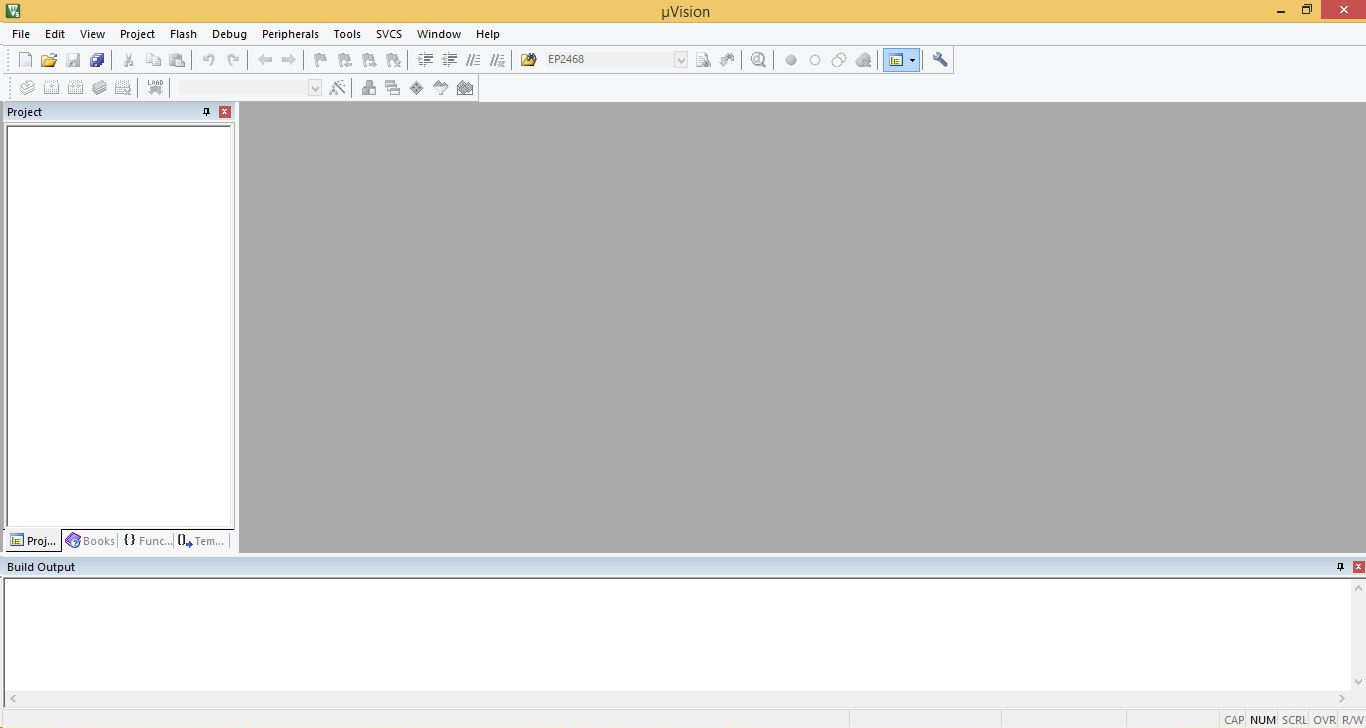
\includegraphics[width=0.7\textwidth]{A1keil.png}
		\caption{Vista inicial de la ventana de Keil $\mu$Vision}
		\label{initkeil}
	\end{figure}
	Cuando el usuario inicia el programa, se encuentra con una ventana como la que se observa en la Figura \ref{initkeil}.%sobre projecto para configurar fx2lp
		\chapter{Archivos de configuración del controlador FX2LP}
	\label{ap:fx2lp}
	En el presente apéndice se detallan los códigos fuente, los cuales fueron escritos en lenguaje C para microcontroladores. Estos códigos se utilizaron para configurar la interfaz FX2LP, incluyendo los archivos:
	\begin{itemize}
		\item \hyperref[ap:fx2lp:ifc]{\textbf{interfaz.c:}} Funciones \verb|TD_Init()|, \verb|TD_Poll()| desarrolladas en este trabajo y funciones necesarias para el correcto funcionamiento del puerto USB, provistas por Cypress Semiconductor.
		\item \hyperref[ap:fx2lp:fwc]{\textbf{fw.c:}} Función \verb|main()| modificada por robustez.
		\item \hyperref[ap:fx2lp:ledh]{\textbf{leds.h:}} Encabezado que contiene los registros necesarios para encender y apagar los LED multipropósito de la placa de desarrollo CY3684 EZ-USB de Cypress Semiconductor.
		\item \hyperref[ap:fx2lp:serh]{\textbf{FX2LPSerial.h:}} Encabezado de la biblioteca utilizada para transmitir datos a través del puerto UART.
		\item \hyperref[ap:fx2lp:serc]{\textbf{FX2LPSerial.c:}} Implementación de las funciones utilizadas para transmitir datos a través del puerto UART.
	\end{itemize}
	
	Además de los archivos que aquí se desarrollan, es necesario utilizar el framework provisto por Cypress~\cite{CypressSemiconductor2020}.
	
	\subsection*{interfaz.c}
		\label{ap:fx2lp:ifc}
		\lstinputlisting[language=C,numbers=left,numberstyle=\tiny,stepnumber=5,language=VHDL,basicstyle=\small,firstnumber=1]{secciones/extras/codigos/uC/bridge.c}
	\subsection*{fw.c}
		\label{ap:fx2lp:fwc}
		\lstinputlisting[language=C,numbers=left,numberstyle=\tiny,stepnumber=5,language=VHDL,basicstyle=\small,firstnumber=1]{secciones/extras/codigos/uC/fw.c}
	\subsection*{leds.h}
		\label{ap:fx2lp:ledh}
		\lstinputlisting[language=C,numbers=left,numberstyle=\tiny,stepnumber=5,language=VHDL,basicstyle=\small,firstnumber=1]{secciones/extras/codigos/uC/leds.h}
		
	\subsection*{FX2LPSerial.h}
		\label{ap:fx2lp:serh}
		\lstinputlisting[language=C,numbers=left,numberstyle=\tiny,stepnumber=5,language=VHDL,basicstyle=\small,firstnumber=1]{secciones/extras/codigos/uC/FX2LPSerial.h}
	\subsection*{FX2LPSerial.c}
		\label{ap:fx2lp:serc}
		\lstinputlisting[language=C,numbers=left,numberstyle=\tiny,stepnumber=5,language=VHDL,basicstyle=\small,firstnumber=1]{secciones/extras/codigos/uC/FX2LPSerial.c}

%\chapter{Uso del programa Cypress USB Control Center}
%	\label{app:cyusb}
%	Se presenta a continuación un breve tutorial que explica como cargar programas en el controlador FX2LP de Cypress a través del software USB Control Center, como así también, la lectura de descriptores, el envío y recepción de paquetes USB.\\
%	
	%codigo de configuracion fx2lp
		\chapter{Archivos de código para implementación en \acrshort{fpga}}
\label{ap:vhdl}

	El presente apéndice contiene el código desarrollado para la implementación de los sistemas en el \acrshort{fpga} Spartan 6 utilizados en este trabajo. Este código fue escrito en lenguaje \acrshort{vhdl}, salvo por el archivo de restricciones, que posee como lenguaje XST, desarrollado por Xilinx para dicho propósito. A su vez, se expone el resumen de síntesis, en donde constan los recursos del \acrshort{fpga} utilizados.
 	El contenido mostrado en este Apéndice contiene el código de los archivos:
 	\begin{itemize}
		\item \textbf{\nameref{ap:vhdl:iffx2}:} Implementación de la \acrfull{mef} a través de la cual se generan las señales de control que comandan la memoria \acrshort{fifo} del controlador FX2LP 
		
		\item \textbf{\nameref{ap:vhdl:meftb}:} Código utilizado para realizar la verificación funcional de la \acrshort{mef}
		
		\item \textbf{\nameref{ap:vhdl:top}:} Implementación del sistema de pruebas. En él se instancia la \acrshort{mef}, la configuración del \acrshort{pll} y la memoria \acrshort{fifo} generada a través de la herramienta \textit{Core Generator} de Xilinx Inc. 
		
		\item \textbf{\nameref{ap:vhdl:toptb}:} Código de verificación funcional del sistema de pruebas 

		\item \textbf{\nameref{ap:vhdl:ucf}:} Archivo de restricciones en donde se le indica al compilador la frecuencia de la señal de entrada al sistema y la asignación de los puertos de Entrada y Salida del sistema desarrollado a los pines del \acrshort{fpga} Spartan 6.

		\item \textbf{\nameref{ap:vhdl:sum}:} Tabla en donde se indica el consumo de recursos de \acrshort{fpga} por parte de la síntesis realizada a través del entorno de desarrollo ISE de Xilinx Inc.
	\end{itemize}


	\subsection*{fx2lp\_interface.vhd}
		\label{ap:vhdl:iffx2}
		\lstinputlisting[language=VHDL,numbers=left,numberstyle=\tiny,stepnumber=5,language=VHDL,basicstyle=\small,firstnumber=1]{secciones/extras/codigos/VHDL/fx2lp_interface.vhd}
	
	\subsection*{mef\_tb.vhd}
		\label{ap:vhdl:meftb}
		\lstinputlisting[language=VHDL,numbers=left,numberstyle=\tiny,stepnumber=5,firstnumber=1,basicstyle=\small,firstnumber=1]{secciones/extras/codigos/VHDL/mef_tb.vhd}
	
	\subsection*{fx2lp\_interface\_top.vhd}
		\label{ap:vhdl:top}
		\lstinputlisting[language=VHDL,numbers=left,numberstyle=\tiny,stepnumber=5,firstnumber=1,basicstyle=\small,firstnumber=1]{secciones/extras/codigos/VHDL/fx2lp_interface_top.vhd}


	\subsection*{top\_tb.vhd}
		\label{ap:vhdl:toptb}
		\lstinputlisting[language=VHDL,numbers=left,numberstyle=\tiny,stepnumber=5,firstnumber=1,basicstyle=\small,firstnumber=1]{secciones/extras/codigos/VHDL/top_tb.vhd}
	
	\subsection*{fx2lp\_interface\_top.ucf}
		\label{ap:vhdl:ucf}
		\lstinputlisting[numbers=left,numberstyle=\tiny,stepnumber=5,firstnumber=1,basicstyle=\small,firstnumber=1]{secciones/extras/UCF/fx2lp_interface_top.ucf}
	\pagebreak	
	\subsection*{Sumario de síntesis}
		\label{ap:vhdl:sum}
		\begin{table}[ht]
	\centering
	\resizebox{\textwidth}{!}{%
	\begin{tabular}{|l|l|l|l|}
		\toprule
		\rowcolor[rgb]{ .6,  .8,  1} \multicolumn{4}{|c|}{\textbf{fx2lp\_interface\_top Project Status (04/23/2020 - 15:52:42)}} \\
		\midrule
		\rowcolor[rgb]{ 1,  1,  .6} \textbf{Project File:} & \cellcolor[rgb]{ 1,  1,  1}Spartan6.xise & \textbf{Parser Errors:} & \cellcolor[rgb]{ 1,  1,  1}No Errors \\
		\midrule
		\rowcolor[rgb]{ 1,  1,  .6} \textbf{Module Name:} & \cellcolor[rgb]{ 1,  1,  1}fx2lp\_interface\_top & \textbf{Implementation State:} & \cellcolor[rgb]{ 1,  1,  1}Placed and Routed \\
		\midrule
		\rowcolor[rgb]{ 1,  1,  .6} \textbf{Target Device:} & \cellcolor[rgb]{ 1,  1,  1}xc6slx9-2tqg144 & \textbf{Errors:} & \multicolumn{1}{l|}{\cellcolor[rgb]{ 1,  1,  1}} \\
		\midrule
		\rowcolor[rgb]{ 1,  1,  .6} \textbf{Product Version:} & \cellcolor[rgb]{ 1,  1,  1}ISE 14.7 & \textbf{Warnings:} & \multicolumn{1}{l|}{\cellcolor[rgb]{ 1,  1,  1}} \\
		\midrule
		\rowcolor[rgb]{ 1,  1,  .6} \textbf{Design Goal:} & \cellcolor[rgb]{ 1,  1,  1}Balanced & \textbf{Routing Results:} & \cellcolor[rgb]{ 1,  1,  1}All Signals Completely Routed \\
		\midrule
		\rowcolor[rgb]{ 1,  1,  .6} \textbf{Design Strategy:} & \cellcolor[rgb]{ 1,  1,  1}Xilinx Default (unlocked) & \textbf{Timing Constraints:} & \cellcolor[rgb]{ 1,  1,  1}All Constraints Met \\
		\midrule
		\rowcolor[rgb]{ 1,  1,  .6} \textbf{Environment:} & \cellcolor[rgb]{ 1,  1,  1}System Settings & \textbf{Final Timing Score:} & \cellcolor[rgb]{ 1,  1,  1}0  (Timing Report) \\
		\bottomrule
	\end{tabular}}%
	\label{tab:pstatus}%
\end{table}%


{\small\tabcolsep=6.5pt
\begin{longtable}{|l|r|r|r|r|}
	\toprule \rowcolor[rgb]{ .6,  .8,  1} \multicolumn{5}{|c|}{\textbf{Device Utilization Summary}}\\
	\midrule
	\rowcolor[rgb]{ 1,  1,  .6} \textbf{Slice Logic Utilization} & \multicolumn{1}{c|}{\textbf{Used}} & \multicolumn{1}{c|}{\textbf{Available}} & \multicolumn{1}{c|}{\textbf{Utilization}} & \multicolumn{1}{c|}{\textbf{Note(s)}} \\
	\midrule
	\endfirsthead
	\toprule \rowcolor[rgb]{ .6,  .8,  1} \multicolumn{5}{|c|}{\textbf{Device Utilization Summary (cont.)}}\\
	\midrule
	\rowcolor[rgb]{ 1,  1,  .6} \textbf{Slice Logic Utilization} & \multicolumn{1}{c|}{\textbf{Used}} & \multicolumn{1}{c|}{\textbf{Available}} & \multicolumn{1}{c|}{\textbf{Utilization}} & \multicolumn{1}{c|}{\textbf{Note(s)}} \\
	\midrule
	\endhead
	\multicolumn{5}{|r|}{Continúa en la siguiente página}\\
	\bottomrule
	\endfoot
	\bottomrule
	\endlastfoot
	Number of Slice Registers & 83    & 11,440 & 1\%   &  \\
	\midrule
	\,\,\,\,\,Number used as Flip Flops & 79    &       &       &  \\
	\midrule
	\,\,\,\,\,Number used as Latches & 4     &       &       &  \\
	\midrule
	\,\,\,\,\,Number used as Latch-thrus & 0     &       &       &  \\
	\midrule
	\,\,\,\,\,Number used as AND/OR logics & 0     &       &       &  \\
	\midrule
	Number of Slice LUTs & 80    & 5,720 & 1\%   &  \\
	\midrule
	\,\,\,\,\,Number used as logic & 79    & 5,720 & 1\%   &  \\
	\midrule
	\,\,\,\,\,\,\,\,\,\,Number using O6 output only & 35    &       &       &  \\
	\midrule
	\,\,\,\,\,\,\,\,\,\,Number using O5 output only & 1     &       &       &  \\
	\midrule
	\,\,\,\,\,\,\,\,\,\,Number using O5 and O6 & 43    &       &       &  \\
	\midrule
	\,\,\,\,\,\,\,\,\,\,Number used as ROM & 0     &       &       &  \\
	\midrule
	\,\,\,\,\,Number used as Memory & 0     & 1,440 & 0\%   &  \\
	\midrule
	\,\,\,\,\,Number used exclusively as route-thrus & 1     &       &       &  \\
	\midrule
	\,\,\,\,\,\,\,\,\,\,Number with same-slice register load & 1     &       &       &  \\
	\midrule
	\,\,\,\,\,\,\,\,\,\,Number with same-slice carry load & 0     &       &       &  \\
	\midrule
	\,\,\,\,\,\,\,\,\,\,Number with other load & 0     &       &       &  \\
	\midrule
	Number of occupied Slices & 39    & 1,430 & 2\%   &  \\
	\midrule
	Number of MUXCYs used & 44    & 2,860 & 1\%   &  \\
	\midrule
	Number of LUT Flip Flop pairs used & 106   &       &       &  \\
	\midrule
	\,\,\,\,\,Number with an unused Flip Flop & 35    & 106   & 33\%  &  \\
	\midrule
	\,\,\,\,\,Number with an unused LUT & 26    & 106   & 24\%  &  \\
	\midrule
	\,\,\,\,\,Number of fully used LUT-FF pairs & 45    & 106   & 42\%  &  \\
	\midrule
	\,\,\,\,\,Number of unique control sets & 14    &       &       &  \\
	\midrule
	\,\,\,\,\,Number of slice register sites lost & \multirow{2}[2]{*}{77} & \multirow{2}[2]{*}{11,440} & \multirow{2}[2]{*}{1\%} & \multirow{2}[2]{*}{} \\
	\,\,\,\,\,\,\,\,\,\,to control set restrictions &       &       &       & \\
	\midrule
	Number of bonded IOBs & 37    & 102   & 36\%  &  \\
	\midrule
	\,\,\,\,\,Number of LOCed IOBs & 36    & 37    & 97\%  &  \\
	\midrule
	\,\,\,\,\,IOB Flip Flops & 1     &       &       &  \\
	\midrule
	\,\,\,\,\,IOB Latches & 16    &       &       &  \\
	\midrule
	Number of RAMB16BWERs & 1     & 32    & 3\%   &  \\
	\midrule
	Number of RAMB8BWERs & 0     & 64    & 0\%   &  \\
	\midrule
	Number of BUFIO2/BUFIO2\_2CLKs & 1     & 32    & 3\%   &  \\
	\midrule
	\,\,\,\,\,Number used as BUFIO2s & 1     &       &       &  \\
	\midrule
	\,\,\,\,\,Number used as BUFIO2\_2CLKs & 0     &       &       &  \\
	\midrule
	Number of BUFIO2FB/BUFIO2FB\_2CLKs & 1     & 32    & 3\%   &  \\
	\midrule
	\,\,\,\,\,Number used as BUFIO2FBs & 1     &       &       &  \\
	\midrule
	\,\,\,\,\,Number used as BUFIO2FB\_2CLKs & 0     &       &       &  \\
	\midrule
	Number of BUFG/BUFGMUXs & 3     & 16    & 18\%  &  \\
	\midrule
	\,\,\,\,\,Number used as BUFGs & 3     &       &       &  \\
	\midrule
	\,\,\,\,\,Number used as BUFGMUX & 0     &       &       &  \\
	\midrule
	Number of DCM/DCM\_CLKGENs & 0     & 4     & 0\%   &  \\
	\midrule
	Number of ILOGIC2/ISERDES2s & 16    & 200   & 8\%   &  \\
	\midrule
	\,\,\,\,\,Number used as ILOGIC2s & 16    &       &       &  \\
	\midrule
	\,\,\,\,\,Number used as ISERDES2s & 0     &       &       &  \\
	\midrule
	Number of IODELAY2/IODRP2/IODRP2\_MCBs & 0     & 200   & 0\%   &  \\
	\midrule
	Number of OLOGIC2/OSERDES2s & 1     & 200   & 1\%   &  \\
	\midrule
	\,\,\,\,\,Number used as OLOGIC2s & 1     &       &       &  \\
	\midrule
	\,\,\,\,\,Number used as OSERDES2s & 0     &       &       &  \\
	\midrule
	Number of BSCANs & 0     & 4     & 0\%   &  \\
	\midrule
	Number of BUFHs & 0     & 128   & 0\%   &  \\
	\midrule
	Number of BUFPLLs & 0     & 8     & 0\%   &  \\
	\midrule
	Number of BUFPLL\_MCBs & 0     & 4     & 0\%   &  \\
	\midrule
	Number of DSP48A1s & 0     & 16    & 0\%   &  \\
	\midrule
	Number of ICAPs & 0     & 1     & 0\%   &  \\
	\midrule
	Number of MCBs & 0     & 2     & 0\%   &  \\
	\midrule
	Number of PCILOGICSEs & 0     & 2     & 0\%   &  \\
	\midrule
	Number of PLL\_ADVs & 1     & 2     & 50\%  &  \\
	\midrule
	Number of PMVs & 0     & 1     & 0\%   &  \\
	\midrule
	Number of STARTUPs & 0     & 1     & 0\%   &  \\
	\midrule
	Number of SUSPEND\_SYNCs & 0     & 1     & 0\%   &  \\
	\midrule
	Average Fanout of Non-Clock Nets & 2.91  &       &       &  \\
\end{longtable}}


\begin{center}
	\centering
	\resizebox{\textwidth}{!}{%
	\begin{tabular}{|l|l|l|l|l|l|}
		\toprule
		\rowcolor[rgb]{ .6,  .8,  1} \multicolumn{6}{|c|}{\textbf{Detailed Reports}}\\
		\midrule
		\rowcolor[rgb]{ 1,  1,  .6} \textbf{Report Name} & \textbf{Status} & \textbf{Generated} & \textbf{Errors} & \textbf{Warnings} & \textbf{Infos} \\
		\midrule
		Synthesis Report & Current & jue 23. abr 15:51:44 2020 & 0     & 26 Warnings (0 new) & 14 Infos (10 new) \\
		\midrule
		Translation Report & Current & jue 23. abr 15:51:53 2020 & 0     & \multicolumn{1}{l|}{0} & 2 Infos (0 new) \\
		\midrule
		Map Report & Current & jue 23. abr 15:52:24 2020 &       & \multicolumn{1}{l|}{} &  \\
		\midrule
		Place and Route Report & Current & jue 23. abr 15:52:34 2020 & 0     & 6 Warnings (0 new) & 0 \\
		\midrule
		Power Report & \multicolumn{1}{l|}{} & \multicolumn{1}{l|}{} &       & \multicolumn{1}{l|}{} &  \\
		\midrule
		Post-PAR Static Timing Report & Current & jue 23. abr 15:52:40 2020 & 0     & \multicolumn{1}{l|}{0} & 3 Infos (0 new) \\
		\midrule
		Bitgen Report & Out of Date & mi\'e 1. abr 14:38:01 2020 & 0     & 4 Warnings (0 new) & 1 Info (0 new) \\
		\bottomrule
	\end{tabular}}%
\end{center}

\begin{center}
	\centering
	\begin{tabular}{c}
		Date Generated: 05/31/2020 - 15:05:40 \\
	\end{tabular}%
\end{center}%

%codigo de vhdl
		\chapter{Código para \acrshort{pc} del programa de pruebas}
	\label{ap:cpp}
	El presente apéndice contiene el código escrito en lenguaje C++, el cual fue desarrollado durante el transcurso del trabajo aquí informado con el objetivo de obtener un programa que transmita datos a través del puerto \acrshort{usb}.
	Los archivos exhibidos en este apéndice son:
	
	\begin{itemize}
		\item \textbf{\nameref{ap:cpp:head}:} Archivo de cabecera utilizado para la declaración de clases y funciones, como así también la definición de variables utilizadas en la ejecución del programa de pruebas
		
		\item \textbf{\nameref{ap:cpp:impl}:} Archivo de implementación del programa de pruebas, en donde se define la función \verb|main()| y las declaradas en el encabezado.
	\end{itemize}

	\subsection*{tfUSBCheck.h}
		\label{ap:cpp:head}
			\lstinputlisting[numbers=left,numberstyle=\tiny,stepnumber=5,language=C++,basicstyle=\small,firstnumber=1]{secciones/extras/codigos/C++/tfUSBCheck.h}
	\subsection*{tfUSBCheck.cpp}
		\label{ap:cpp:impl}
			\lstinputlisting[numbers=left,numberstyle=\tiny,stepnumber=5,language=C++,basicstyle=\small,firstnumber=1]{secciones/extras/codigos/C++/tfUSBCheck.cpp}%codigo cpp
		\chapter{Esquemático de la Placa de Interconexión}
	\label{ap:pcb}
	\begin{center}
		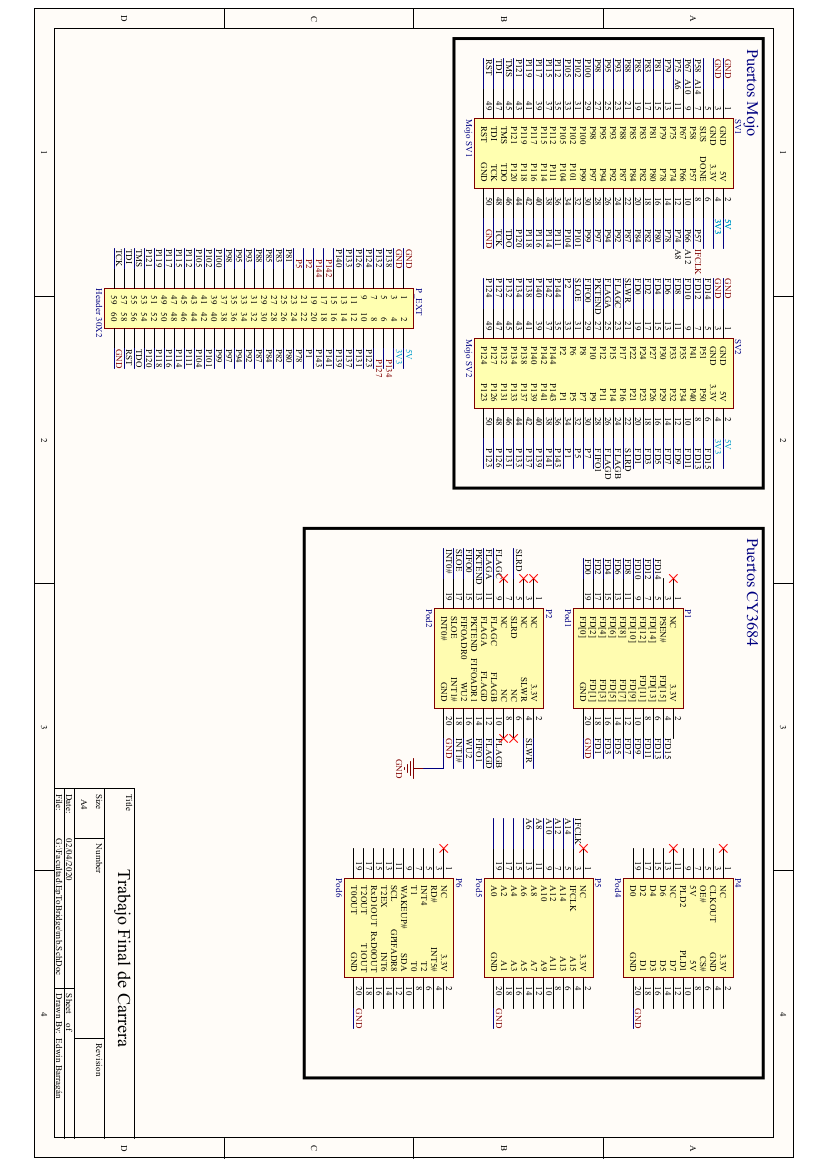
\includegraphics[height=.78\textheight]{secciones/extras/PCB/esquematicoPCB.png}
	\end{center}
%esquematico pcb
	\end{appendices}
\end{document}